\documentclass{memoir}

\usepackage{amsthm,amssymb,amsmath}
\usepackage{makeidx}
\usepackage{xifthen}
\usepackage[inline]{enumitem}
\usepackage{tikz}
  \usetikzlibrary{patterns}
  \usetikzlibrary{cd}
  \usetikzlibrary{calc}
  \usetikzlibrary{arrows}
\usepackage[framemethod=tikz,usetwoside]{mdframed}
\usepackage{hyperref}
  \hypersetup{linktocpage,colorlinks,linkcolor=blue}
\usepackage[figurewithin=section]{caption}
\usepackage{collect}
\usepackage{wasysym}
\usepackage{mathtools}

% #Counters
%

%-----------%
% #Counters %
%-----------%

% Number chapters as I, II, III, etc.
\renewcommand{\thechapter}{\Roman{chapter}}

% Number sections sequentially (not within chapters)
\counterwithout{section}{chapter}

% Number figures and tables within sections
\makeatletter                        %&%
  \renewcommand\@memmain@floats{     %&%
    \counterwithout{figure}{chapter} %&%
    \counterwithin{figure}{section}  %&%
    \counterwithout{table}{chapter}  %&%
    \counterwithin{table}{section}   %&%
  }                                  %&%
\makeatother                         %&%




%%%


% Keep chapter numbers and titles from overlapping in TOC
\renewcommand{\chapternumberlinebox}[2]{\makebox[1cm][l]{#2}}

% Roman-enumerated lists for propositions and proofs
\newenvironment{proplist}[0] %&%
  {\begin{enumerate}[(i)]}   %&%
  {\end{enumerate}}          %&%

\newenvironment{proplist*}[0]                        %&%
  {\begin{enumerate}[(i)] \setlength{\itemsep}{0pt}} %&%
  {\end{enumerate}}                                  %&%

\newenvironment{inlineproplist}[0] %&%
  {\begin{inparaenum}[(i)]}        %&%
  {\end{inparaenum}}               %&%

% Subreferences
\newcommand{\sref}[2]{\ref{#1}(\ref{#1:#2})}
\newcommand{\paref}[1]{(\ref{#1})}
\newcommand{\eref}[1]{\hyperref[#1]{Exercise \ref*{#1}}}
\newcommand{\propref}[1]{\hyperref[#1]{Proposition \ref*{#1}}}


% Page style
\makepagestyle{standard} %&%

\makeatletter                                                  %&%
\makeevenfoot{standard}{}{}{}                                  %&%
\makeoddfoot{standard}{}{}{}                                   %&%
\makeevenhead{standard}{\bfseries\thepage}{}{\rightmark}       %&%
\makeoddhead{standard}{\leftmark}{}{\bfseries\thepage}         %&%
\makeheadrule{standard}{\textwidth}{\normalrulethickness}      %&%
\makefootrule{standard}{\textwidth}{\normalrulethickness}{0ex} %&%
\makeatother                                                   %&%

\renewcommand*{\sectionmark}[1]{                      %&%
  \markboth{\S\thesection: {#1}}{\S\thesection: {#1}} %&%
}                                                     %&%

\nouppercaseheads    %&%
\pagestyle{standard} %&%
\chapterstyle{dash}  %&%

% Theorem styles
\theoremstyle{definition}                 %&%
\newtheorem{dfn}{Def'n}[section]          %&%
\newtheorem{thm}[dfn]{Theorem}            %&%
\newtheorem{cor}[dfn]{Cor.}               %&%
\newtheorem{prop}[dfn]{Prop'n}            %&%
\newtheorem{lem}[dfn]{Lemma}              %&%
\newtheorem{construct}[dfn]{Construction} %&%
\newtheorem{axiom}[dfn]{Axiom}            %&%

% Exercises
\newcommand{\Exercises}{\par\bigskip\noindent\hfill{\textasteriskcentered\quad\textasteriskcentered\quad\textsc{\large Exercises}\quad\textasteriskcentered\quad\textasteriskcentered}\hfill\null\par\bigskip}

\newcounter{dummycounter}         %&%
\newcounter{exercise}[section]    %&%
\counterwithin{exercise}{section} %&%

\marginparmargin{left} %&%

\newenvironment{exercise}[1][\unskip]{                     %&%
  \refstepcounter{exercise}                                %&%
  \par\noindent\marginpar{\hfill\theexercise .}\textbf{#1} %&%
}{                                                         %&%
  \medskip                                                 %&%
}                                                          %&%



% Examples
\newenvironment{examples}{                      %&%
  \par\bigskip\noindent\textbf{\large Examples} %&%
  \begin{enumerate}                             %&%
}{                                              %&%
  \end{enumerate}                               %&%
}                                               %&%


\mdfdefinestyle{mystyle}{ %&%
  hidealllines=true,      %&%
  leftline=true,          %&%
  innerleftmargin=10pt,   %&%
  innerrightmargin=10pt,  %&%
  innertopmargin=0pt,     %&%
}                         %&%

\surroundwithmdframed[style=mystyle]{dfn}   %&%
\surroundwithmdframed[style=mystyle]{prop}  %&%
\surroundwithmdframed[style=mystyle]{cor}   %&%
\surroundwithmdframed[style=mystyle]{axiom} %&%

\def\chapterautorefname{Chapter} %&%
\def\sectionautorefname{Section} %&%
\def\figureautorefname{Figure}   %&%


% For nebulous "problem" statements
\newenvironment{titlebox}[1]                       %&%
  {\mdfsetup{                                      %&%
    frametitle={\colorbox{white}{\space#1\space}}, %&%
    innertopmargin=7pt,                            %&%
    innerbottommargin=10pt,                        %&%
    frametitleaboveskip=-\ht\strutbox,             %&%
    frametitlealignment=\center                    %&%
    }                                              %&%
  \begin{mdframed}                                 %&%
  }                                                %&%
  {\end{mdframed}                                  %&%
}                                                  %&%


%---------%
% Numbers %
%---------%

\newcommand{\ZZ}{\ensuremath{\mathbb{Z}}} %&%
\newcommand{\NN}{\ensuremath{\mathbb{N}}} %&%
\newcommand{\QQ}{\ensuremath{\mathbb{Q}}} %&%
\newcommand{\RR}{\ensuremath{\mathbb{R}}} %&%
\newcommand{\CC}{\ensuremath{\mathbb{C}}} %&%

\newcommand{\ZZINT}[2]{\ensuremath{[\![#1,#2]\!]}} %&%



%-----------------------%
% Maps and sets of maps %
%-----------------------%

\newcommand{\ID}[1][]{\ensuremath{ %&%
  \ifthenelse{\isempty{#1}}        %&%
    {\mathsf{id}}                  %&%
    {\mathsf{id}_{#1}}             %&%
}}                                 %&%

\newcommand{\END}[1]{\ensuremath{ %&%
  \mathsf{End}\left(#1\right)     %&%
}}                                %&%

\newcommand{\ENDU}[1]{\ensuremath{ %&%
  \mathsf{End}_1\left(#1\right)    %&%
}}                                 %&%



%--------------%
% Ring subsets %
%--------------%

\newcommand{\CENTER}[1]{\ensuremath{ %&%
  Z\left(#1\right)                   %&%
}}                                   %&%

\newcommand{\NILRADICAL}[1]{\ensuremath{ %&%
  N\left(#1\right)                       %&%
}}                                       %&%

\newcommand{\UNITS}[1]{\ensuremath{ %&%
  \mathcal{U}\left(#1\right)        %&%
}}                                  %&%

\newcommand{\KER}[1]{\ensuremath{ %&%
  \mathsf{ker}(#1)                %&%
}}                                %&%

\newcommand{\IM}[1]{\ensuremath{ %&%
  \mathsf{im}(#1)                %&%
}}                               %&%



%--------------------------%
% Families of ring subsets %
%--------------------------%

\newcommand{\ASSOCLAT}[1]{\ensuremath{ %&%
  \mathcal{A}\left(#1\right)           %&%
}}                                     %&%

\newcommand{\IDEALS}[2][]{\ensuremath{ %&%
  \ifthenelse{\isempty{#1}}            %&%
    {\mathcal{Q}\left(#2\right)}       %&%
    {\mathcal{Q}_{#1}\left(#2\right)}  %&%
}}                                     %&%



%----------%
% Geometry %
%----------%

\newcommand{\COLLINEAR}[3]{\ensuremath{\langle #1, #2, #3 \rangle}}%&%
\newcommand{\LINE}[2]{\ensuremath{\overleftrightarrow{#1#2}}}%&%
\newcommand{\BETWEEN}[3]{\ensuremath{[ #1 #2 #3 ]}}%&%
\newcommand{\SEGMENT}[2]{\ensuremath{\overline{#1#2}}}%&%
\newcommand{\RAY}[2]{\ensuremath{\overrightarrow{#1#2}}}%&%
\newcommand{\TRIANGLE}[3]{\ensuremath{\bigtriangleup{#1#2#3}}}%&%
\newcommand{\ANGLE}[3]{\ensuremath{\angle{#1#2#3}}}%&%
\newcommand{\INTANGLE}[3]{\ensuremath{\mathsf{int}\angle{#1#2#3}}}%&%
\newcommand{\SEGCONG}[4]{\ensuremath{(#1,#2) \cong_s (#3,#4)}}%&%
\newcommand{\ANGCONG}[6]{\ensuremath{(#1,#2,#3) \cong_a (#4,#5,#6)}}%&%
\renewcommand{\CIRCLE}[2]{\ensuremath{\ocircle{#1#2}}}%&%
\newcommand{\INTCIRCLE}[2]{\ensuremath{\mathsf{int}\CIRCLE{#1}{#2}}}
\newcommand{\EXTCIRCLE}[2]{\ensuremath{\mathsf{ext}\CIRCLE{#1}{#2}}}

\newcommand{\HALFPLANEA}[1]{\mathcal{H}_{1,\ell}}
\newcommand{\HALFPLANEB}[1]{\mathcal{H}_{2,\ell}}

\newcommand{\SEPARATE}[4]{\ensuremath{(#1,#2 \mid #3,#4)}}

\newcommand{\HYPHP}{\ensuremath{\mathbb{H}}}
\newcommand{\HHPIDEALPOINT}[2]{\ensuremath{H_{#1,#2}}}

\newcommand{\POINCAREDISC}{\ensuremath{\mathbb{P}}}
\newcommand{\PDDET}[2]{D_{#1,#2}}
\newcommand{\PDIDEALPOINT}[2]{P_{#1,#2}}

\newcommand{\KLEINDISC}{\ensuremath{\mathbb{K}}}
\newcommand{\KDIDEALPOINT}[2]{\ensuremath{K_{#1,#2}}}

\newcommand{\EUCLIDEANDISC}{\ensuremath{\mathbb{E}}}

\newcommand{\ANTIPODALSPHERE}{\ensuremath{\mathbb{A}}}

\newcommand{\MIN}{\ensuremath{\mathsf{min}}}
\newcommand{\MAX}{\ensuremath{\mathsf{max}}}



\newcommand{\SYM}[1]{\ensuremath{\mathsf{Sym}(#1)}}



\newcommand{\TOT}[1]{\ensuremath{\mathsf{tot}\left(#1\right)}}%&%

\newcommand{\POW}[1]{\ensuremath{\mathcal{P}\left(#1\right)}}%&%
\newcommand{\POWP}[1]{\ensuremath{\mathcal{P}_{\!\neq\!}\left(#1\right)}}%&%
\newcommand{\POWF}[1]{\ensuremath{\mathcal{P}_F\left(#1\right)}}%&%

\newcommand{\ZZQUAD}[1]{\ensuremath{\mathcal{O}(\sqrt{#1})}}%&%
\newcommand{\ZZFRAC}[1]{\ensuremath{{#1}^{-1}\ZZ}}%&%

\newcommand{\ION}[1]{\ensuremath{\mathsf{nilp}\left(#1\right)}}%&%

\newcommand{\REXTEND}[3]{\ensuremath{#1 \rtimes_{#2} #3}}%&%
\newcommand{\ADJUNIT}[1]{\ensuremath{{#1}^{(1)}}}%&%
\newcommand{\HAM}[1]{\ensuremath{\mathbb{H}(#1)}}%&%

\newcommand{\ADDORD}[1]{\ensuremath{\mathsf{ord}\left(#1\right)}}%&%
\newcommand{\CHAR}[1]{\ensuremath{\mathsf{char}(#1)}}%&%

\newcommand{\MAT}[2]{\ensuremath{\mathsf{Mat}_{#1}(#2)}}%&%
\newcommand{\UTMAT}[2]{\ensuremath{\mathsf{UT}_{#1}(#2)}}%&%
\newcommand{\LTMAT}[2]{\ensuremath{\mathsf{LT}_{#1}(#2)}}%&%
\newcommand{\DIAGMAT}[2]{\ensuremath{\mathsf{Diag}_{#1}(#2)}}%&%
\newcommand{\DET}{\ensuremath{\mathsf{det}}}%&%

\newcommand{\GCD}[2]{\ensuremath{\mathsf{gcd}(#1, #2)}}%&%
\newcommand{\LCM}[2]{\ensuremath{\mathsf{lcm}(#1, #2)}}%&%
\newcommand{\GCDS}[1]{\ensuremath{\mathsf{gcd}\left(#1\right)}}%&%

\newcommand{\CONTENT}[1]{\ensuremath{\mathsf{content}(#1)}}%&%

\newcommand{\ASSOC}{\ensuremath{\approx}}%&%
\newcommand{\COPRIME}{\ensuremath{\perp}}%&%

\newcommand{\DIVORD}[2]{\ensuremath{\mathsf{div}_{#1}\left(#2\right)}}%&%

\newcommand{\LOCALIZE}[2]{\ensuremath{{#2}^{-1}{#1}}}%&%

\newcommand{\POLYEVAL}[1]{\ensuremath{\varepsilon_{#1}}}%&%
\newcommand{\DERIV}[1][]{\ensuremath{\ifthenelse{\isempty{#1}}{\mathsf{D}}{\mathsf{D}_{#1}}}}%&%

\newcommand{\TILDE}[1]{\ensuremath{\widetilde{#1}}}%&%

\newcommand{\LIM}[2][]{\ensuremath{\ifthenelse{\isempty{#1}}{\lim}{\lim_{#1}}\left(#2\right)}}%&%

\newcommand{\VALCOMP}[2]{\ensuremath{\overline{#1}_{#2}}}%&%


\makeindex

\begin{document}

\frontmatter%
  \thispagestyle{empty}

\vspace{4cm}

\begin{center}
\Large algebra party time

\large rings edition
\end{center}

\vspace{10cm}

\begin{center}
nathan bloomfield
\end{center}


  \begin{center}
\begin{minipage}{0.8\textwidth}
\begin{center}
This work is licensed under a Creative Commons Attribution NonCommercial ShareAlike 4.0 International License.

\vspace{12pt}

\includegraphics[scale=0.8]{src/ring/gfx/by-nc-sa.eps}
\end{center}
\end{minipage}
\end{center}

    \newpage

  \tableofcontents%
  \chapter{Preface}
    These are the lecture notes of a first abstract algebra course the author teaches at the Northeastern State University of Oklahoma.
Each section is intended to be one-half to one class meeting's worth of material.

As these are functionally lecture notes, used in a specific class, the main expository sections develop only the basic theory of rings as dictated by the needs of my students.
Plenty of supplementary material, including some important definitions and theorems, is relegated to the ``exercises''.
The exercises come in a few flavors: some are straight computation, some ask for examples or counterexamples, and some require a proof.
Some exercises -- my favorites -- will guide you through the proofs of reasonably high-powered theorems.
Motivated readers are encouraged to work as many of these as they can stand.

Some additional supplementary material, appropriate to the main text but cut from a typical class due to time constraints, is given in the appendices.
These include constructions of the real, complex, and \(p\)-adic numbers, Zorn's lemma, and a brief discussion of categories.


  \chapter{Introduction}
    These notes develop the basic theory of \textbf{rings}, which grew over time out of several historical threads.
Mathematicians of ``antiquity'' (defined here as the period from prehistory to the Enlightenment) were broadly interested in solving equations of several different kinds.
For example, Diophantine equations like \(a^2 + b^2 = c^2\), of which we are only interested in integer solutions.
Or polynomial equations such as \(ax^2 + bx + c = 0\), where \(a\), \(b\), and \(c\) are known constants.
Or systems of simultaneous linear equations.
Over time techniques were discovered for understanding various types of equations, and by the 19th Century these techniques had developed into fairly sophisticated branches of mathematics.
Diophantine equations became the motivation for a nascent Algebraic Number Theory, whose great white whale was Fermat's Last Theorem.
The rich history of polynomial equations reached an apex with the Abel-Ruffini Theorem on the insolubility of the general quintic equation.
And the study of simultaneous linear equations evolved into what we now call Linear and Multilinear Algebra at the hands of Hermann Grassmann and was used to simplify many ideas in geometry and physics.
\begin{figure}[h!]
\begin{center}
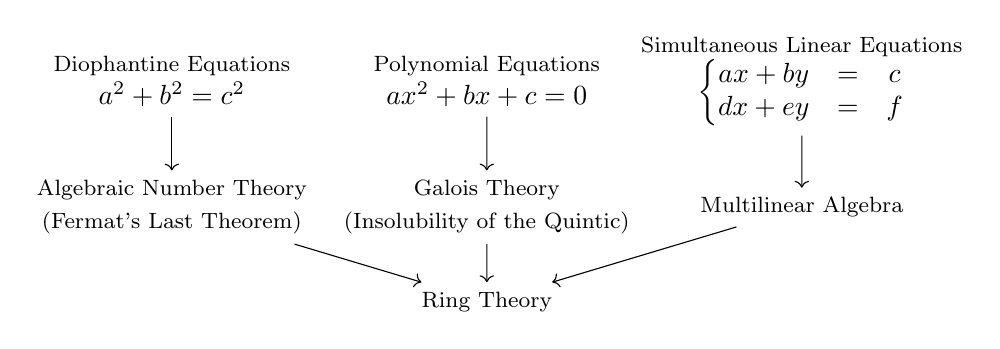
\begin{tikzpicture}[scale=0.8]
  \node[align=center] (num) at (0,3.5)
    {\footnotesize Diophantine Equations \\ \(a^2 + b^2 = c^2\)};
  \node[align=center] (pol) at (5,3.5)
    {\footnotesize Polynomial Equations \\ \(ax^2 + bx + c = 0\)};
  \node[align=center] (mat) at (10,3.5)
    {\footnotesize Simultaneous Linear Equations \\ 
      \(\left\{ \begin{matrix} ax + by & = & c \\ dx + ey & = & f \end{matrix} \right.\)};

  \node[align=center] (ant) at (0,1.5)
    {\footnotesize Algebraic Number Theory \\ \footnotesize (Fermat's Last Theorem)};
  \node[align=center] (gal) at (5,1.5)
    {\footnotesize Galois Theory \\ \footnotesize (Insolubility of the Quintic)};
  \node[align=center] (lin) at (10,1.5)
    {\footnotesize Multilinear Algebra};

  \node[align=center] (rin) at (5,0)
    {\footnotesize Ring Theory};

  \draw[->] (num) -- (ant);
  \draw[->] (pol) -- (gal);
  \draw[->] (mat) -- (lin);

  \draw[->] (ant) -- (rin);
  \draw[->] (gal) -- (rin);
  \draw[->] (lin) -- (rin);
\end{tikzpicture}
\end{center}
\caption{A grossly oversimplified genealogy of ring theory.}
\end{figure}
Underlying these more-or-less parallel developments was a common abstraction, which we call a \emph{ring}, and which was only made explicit in the first couple of decades of the 20th Century.
\textbf{The essence of `ringhood' is the structure -- the arithmetic -- that the integers, polynomials, and square matrices have in common.}

The content of these notes is usually covered in a class called ``Abstract Algebra'', a name which I dislike for two reasons.
First, \textbf{all} mathematics is abstract.
Yes, even the so-called ``applied'' branches.
To single out only some ideas as being abstract is not a useful distinction.
It can even hurt; many students reflexively recoil at ``abstract'' subjects as being inherently pointless and useless.
The second reason for my dislike of the name ``abstract algebra'' is that, reason one notwithstanding, algebra is jam-packed with concrete objects which we can fiddle with and compute and draw pictures of.
In fact the whole purpose of the ``abstract'' part is so that we can better understand the ``concrete'' part.

Yet the name persists, and is not likely to go away soon (if for no other reason than that it takes an act of nature to change a university catalog).
This name reflects a central tension between two broad points of view in mathematics: the abstract and the concrete.
The abstract point of view prefers theory-building; it likes for theorems to be as general as possible; and it doesn't mind nonconstructive proofs, especially if they are slick or insightful.
The concrete point of view really likes constructive results; it tries to keep an eye on specific examples; and is never happier than when a proof can be interpreted as a clear and efficient algorithm.
Neither point of view has a monopoly on enlightenment.
The abstract point of view needs interesting concrete examples to abstract away from, and the concrete point of view is quickly bogged down in irrelevant details without abstraction.
I have tried to balance these two perspectives here.
In your development as a mathematical thinker, it is vital that you become comfortable using both perspectives.

\begin{center}
\begin{minipage}{0.7\textwidth}
Two monks were arguing about a flag.

One said: ``The flag is moving.''

The other said: ``The wind is moving.''

The sixth patriarch happened to be passing by. He told them: ``Not the wind, not the flag; mind is moving.''

\hfill \emph{The Gateless Gate}, Case 29
\end{minipage}
\end{center}


  % Introductory chapters
  \chapter{Preliminaries}
    \section{Sets}
      Here we \textbf{briefly} review some basic ideas from the naive theory of sets.

\begin{proplist}
\item \emph{Set} is an undefined term.

\item There is an undefined predicate \(\in\) among sets, pronounced ``is an element of'', such that given two sets \(A\) and \(B\) the statement \(A \in B\) is either true or false.

\item There is a set \(\varnothing\), called the \emph{empty set}, such that \(x \in \varnothing\) is false for all \(x\).

\item Given two sets \(A\) and \(B\), we say \(A\) is a \emph{subset} of \(B\), denoted \(A \subseteq B\), if for all sets \(x\), \(x \in A\) implies \(x \in B\).

\item If \(A\) is a set, then there is a set \(\POW{A}\), called the \emph{powerset}\index{powerset} of \(A\), such that \(x \in \POW{A}\) if and only if \(x \subseteq A\).

\item Given two sets \(A\) and \(B\), we say \(A\) is \emph{equal to} \(B\) if \(A \subseteq B\) and \(B \subseteq A\).

\item If \(a\) and \(b\) are sets, there is a set \((a,b)\) called the \emph{ordered pair} with \emph{first coordinate} \(a\) and \emph{second coordinate} \(b\).

\item If \(A\) and \(B\) are sets, there is a set \(A \times B\), called the \emph{cartesian product} of \(A\) and \(B\), such that \(x \in A \times B\) if and only if \(x = (a,b)\) for some \(a \in A\) and \(b \in B\).

\item Let \(A\) and \(B\) be sets, with \(B \neq \varnothing\).
A subset \(f \subseteq A \times B\) is called a \emph{function}\index{function} or \emph{mapping} if
\begin{proplist}
\item \(f\) is \emph{total}: for every \(a \in A\), there exists a \(b \in B\) such that \((a,b) \in f\)
\item \(f\) is \emph{well-defined}: if \((a_1,b_1)\) and \((a_2,b_2)\) are in \(f\) such that \(a_1 = a_2\), then \(b_1 = b_2\).
\end{proplist}
In this case we say \(f\) is a function \emph{from} \(A\) \emph{to} \(B\), denoted \(f : A \rightarrow B\).
We say that \(A\) is the \emph{domain} of \(f\) and that \(B\) is the \emph{codomain} of \(f\).
Note that if \(f\) is a function from \(A\) to \(B\), then for every \(a \in A\) there exists a unique \(b \in B\) such that \((a,b) \in f\).
We call this \(b\) the \emph{image} of \(a\) under \(f\), denoted \(f(a)\).

\item Let \(f : A \rightarrow B\) be a function.
\begin{proplist}
\item We say \(f\) is \emph{injective}\index{injective} (also known as ``one-to-one'') if whenever \(a_1, a_2 \in A\) such that \(f(a_1) = f(a_2)\), in fact \(a_1 = a_2\).
\item We say \(f\) is \emph{surjective}\index{surjective} (also known as ``onto'') if for every \(b \in B\), there exists an \(a \in A\) such that \(f(a) = b\).
\item We say \(f\) is \emph{bijective}\index{bijective} if it is both injective and surjective.
\end{proplist}

\item If \(A\) is a set, then subsets of \(A \times A\) are called \emph{binary relations} on \(A\).
If \(\sigma\) is a binary relation on \(A\), we will typically write \(x \,\sigma\, y\) rather than \((x,y) \in \sigma\).

\item Let \(A\) be a set and \(\sigma\) a binary relation on \(A\).
We say that \(\sigma\) is a \emph{partial order}\index{partial order} on \(A\) if
\begin{proplist}
\item \(\sigma\) is \emph{reflexive}: \(a \,\sigma\, a\) for all \(a \in A\).
\item \(\sigma\) is \emph{antisymmetric}: If \(a \,\sigma\, b\) and \(b \,\sigma\, a\), then \(a = b\).
\item \(\sigma\) is \emph{transitive}: If \(a \,\sigma\, b\) and \(b \,\sigma\, c\), then \(a \,\sigma\, c\).
\end{proplist}

\item Let \(A\) be a set and \(\sigma\) a binary relation on \(A\).
We say that \(\sigma\) is an \emph{equivalence}\index{equivalence} if
\begin{proplist}
\item \(\sigma\) is \emph{reflexive}: \(a \,\sigma\, a\) for all \(a \in A\).
\item \(\sigma\) is \emph{symmetric}: If \(a \,\sigma\, b\) then \(b \,\sigma\, a\).
\item \(\sigma\) is \emph{transitive}: If \(a \,\sigma\, b\) and \(b \,\sigma\, c\), then \(a \,\sigma\, c\).
\end{proplist}

\item If \(A\) is a set, then the functions from \(A \times A\) to \(A\) are called \emph{binary operations} on \(A\).
If \(f\) is a binary operation on \(A\), we will typically write \(x \,f\, y\) rather than \(f(x,y)\).
\end{proplist}



\mainmatter
  \setcounter{chapter}{-1}

  \chapter{Review of Arithmetic}
    \label{chap:arithmetic}
    A large amount of the material in this text is motivated by some basic ideas in number theory.
In the interest of remaining self-contained, this chapter very briefly covers a few of these ideas.
Some will be familiar, some not.
The proofs here can be safely skipped over on the first reading.

    \newpage

    \section{The Integers}
      \label{sec:the-integers}
      We begin with a formal definition of the set of numbers we call \emph{integers}.

\begin{axiom}[The Integers]
There is a set \(\ZZ\), whose elements are called \emph{integers}\index{integer}, which is equipped with two special distinct elements 0 (called \emph{zero}) and 1 (called \emph{one}), two binary operations \(+\) (called \emph{plus}) and \(\cdot\) (called \emph{times}, and typically not written explicitly) and a binary relation \(\leq\) (pronounced ``is less than or equal to'') which together satisfy the following properties.
\begin{proplist*}
\item[A1.] Plus is \emph{associative}: \((a+b)+c = a+(b+c)\) for all \(a,b,c \in \ZZ\).
\item[A2.] Zero is \emph{neutral} with respect to plus: \(a+0 = 0+a = a\) for all \(a \in \ZZ\).
\item[A3.] Every integer has an \emph{additive inverse}: for every \(a \in \ZZ\) there is an element \(-a \in \ZZ\) (called a \emph{negative} of \(a\)) such that \(a+(-a) = (-a)+a = 0\).
\item[A4.] Plus is \emph{commutative}: \(a+b = b+a\) for all \(a,b \in \ZZ\).
\item[M.] Times is \emph{associative}: \((ab)c = a(bc)\) for all \(a,b,c \in \ZZ\).
\item[D.] Times \emph{distributes over} plus from either side: \(a(b+c) = ab + ac\) and \((b+c)a = ba + ca\) for all \(a,b,c \in \ZZ\).
\item[C.] Times is \emph{commutative}: \(ab = ba\) for all \(a,b \in \ZZ\).
\item[U.] One is \emph{neutral} with respect to times: \(1 \cdot a = a \cdot 1 = a\) for all \(a \in \ZZ\).
\item[P1.] \(a \leq a\) for all \(a \in \ZZ\).
\item[P2.] If \(a \leq b\) and \(b \leq c\), then \(a \leq c\), for all \(a,b,c \in \ZZ\).
\item[P3.] If \(a \leq b\) and \(b \leq a\), then \(a = b\) for all \(a,b \in \ZZ\).
\item[T.] If \(a,b \in \ZZ\), then either \(a \leq b\) or \(b \leq a\).
\item[O1.]\label{ax:o1} If \(a \leq b\) then \(a+c \leq b+c\) for all \(a,b,c \in \ZZ\).
\item[O2.]\label{ax:o2} If \(0 \leq a\) and \(0 \leq b\) then \(0 \leq ab\).
\item[O3.] \(0 \leq 1\).
\item[WOP.] Suppose \(S\) is a nonempty subset of \(\ZZ\) which is bounded below; say \(b \in \ZZ\) has the property that \(b \leq s\) for all \(s \in S\).
Then there is an integer \(m \in S\) such that \(m \leq s\) for all \(s \in S\).
That is, every nonempty subset of \(\ZZ\) which is bounded below has a least element.
This is called the \emph{well-ordering property}\index{well-ordering property} of \(\ZZ\).
\end{proplist*}
\end{axiom}

As usual, \(a < b\) is short for \(a \leq b\) and \(a \neq b\); \(a \geq b\) is equivalent to \(b \leq a\), and \(a > b\) is equivalent to \(b < a\).

It may seem silly to introduce such a large ``axiom''.
Indeed, it is possible to build up the integers out of simpler objects.
However, doing so is not necessary for our purposes.
In developing any axiomatic system there is a balance to be struck between \emph{simplicity of axioms} and \emph{distance to interesting results}.
Taking the existence of \(\ZZ\) as an axiom does not sacrifice too much simplicity -- it is ``only'' one axiom -- but allows us to say useful things very quickly.

Most of the properties of \(\ZZ\) are familiar.
The least intuitive is probably the last one, the well-ordering property.
While strange at first, this property is extremely important.
For example, we can use it to establish this ``obvious'' result.

\begin{prop}
There is no integer \(t\) such that \(0 < t\) and \(t < 1\).
\end{prop}

\begin{proof}
Let \(S = \{ t \in \ZZ \mid 0 < t \ \mathrm{and}\ t < 1 \}\), and suppose that \(S\) is not empty.
Note that \(S\) is bounded below by \(0\) by definition; if \(t \in S\) then \(0 < t\).
By WOP, then, \(S\) must have a least element; say \(m\).
Since \(0 < m\), we have \(0 < mm\) by \ref{ax:o2}.
On the other hand, since \(0 < m\) and \(m < 1\), we have \(mm < m\) by \ref{ax:o1}.
That is, \(mm \in S\), and \(mm < m\) -- a contradiction.
\end{proof}

It is not too hard to show that every integer \(a\) satisfies exactly one of \(a > 0\), \(a = 0\), and \(a < 0\), a result we call the Trichotomy property.
As usual if \(a > 0\) we say \(a\) is \emph{positive} and if \(a < 0\) we say \(a\) is \emph{negative}, and zero is neither positive nor negative.
The nonnegative integers are special enough that we give them a name.

\begin{dfn}[The Natural Numbers]
We denote by \(\NN\) the set of all integers \(n\) such that \(n \geq 0\).
Elements of \(\NN\) are called \emph{natural numbers}\index{natural number}.
\end{dfn}

Now the natural numbers satisfy a nice structural property.

\begin{prop}
If \(n \in \NN\), then either \(n = 0\) or \(n = m+1\) for some \(m \in \NN\).
\end{prop}

\begin{proof}
Suppose \(n \in \NN\) and \(n \neq 0\); then \(n > 0\).
Let \(m = n-1\).
Now if \(m < 0\), we have \(n-1 < 0 < n\), and thus \(0 < 1-n < 1\), a contradiction.
By trichotomy, either \(m = 0\) or \(m > 0\); that is, \(m \in \NN\).
\end{proof}

The well-ordering property of \(\ZZ\) gives us a very powerful tool for working with natural numbers, called the Principle of Mathematical Induction.

\begin{prop}[Principle of Mathematical Induction]
Let \(B \subseteq \NN\).
If \(B\) satisfies the following two properties:
\begin{proplist}
\item \(0 \in B\), and
\item If \(n \in B\), then \(n+1 \in B\);
\end{proplist}
then \(B = \NN\).
\end{prop}

\begin{proof}
We will prove this result by contradiction.
Let \(S = \{ n \in \NN \mid n \not\in B \}\), and suppose \(S\) is not empty.
Then by the Well-Ordering Property, \(S\) has a least element; say \(t\).
Since \(t \in \NN\), either \(t = 0\) or \(t = u+1\) for some \(u \in \NN\).
Since \(0 \in B\), it must be the case that \(t = u+1\).
Note that since \(u < t\), and \(t\) is minimal among the natural numbers which are not in \(B\), we have \(u \in B\).
But then \(t = u+1 \in B\), a contradiction.
So in fact \(S\) is empty and we have \(B = \NN\).
\end{proof}

The Principle of Mathematical Induction (also called just ``induction'' or PMI) gives us a straightforward way to show that a given statement is true for all natural numbers.
Proofs using PMI require two steps: the Base Case (\(0 \in B\)) and the Inductive Step (if \(n \in B\) then \(n+1 \in B\)).
Most importantly, constructive proofs by induction can be turned into \emph{recursive algorithms} which actually compute things.
This is a powerful idea with implications far beyond numbers.



%---------%
\Exercises%
%---------%

\begin{exercise}[Trichotomy.]\label{exerc:trichotomy}
Show that if \(a \in \ZZ\), then exactly one of \(a < 0\), \(a = 0\), or \(a > 0\) is true.
\end{exercise}

\begin{exercise}
Show that the following hold for all \(a,b \in \ZZ\).
\begin{proplist*}
\item If \(a \geq 0\) and \(b \leq 0\) then \(ab \leq 0\).
\item If \(a \leq 0\) and \(b \leq 0\) then \(ab \geq 0\).
\end{proplist*}
\end{exercise}

\begin{exercise}
Show that if \(a\) and \(b\) are integers and \(ab = 1\), then either \(a = b = 1\) or \(a = b = -1\).
(Hint: Apply \eref{exerc:trichotomy} to \(a\).)
\end{exercise}

\begin{exercise}
Show that if \(n \in \NN\) then \[ \sum_{k=1}^n k = \frac{n(n+1)}{2}. \]
\end{exercise}

\begin{exercise}
Show that if \(n \in \NN\) then \[ \sum_{k=1}^n k^2 = \frac{n(n+1)(2n+1)}{6}. \]
\end{exercise}

\begin{exercise}
Show that if \(n \in \NN\) then \[ \sum_{k=1}^n (2k - 1) = n^2. \]
\end{exercise}

\begin{exercise}
Show that if \(n \in \NN\) then \[ \sum_{k=1}^n \frac{1}{k(k+1)} = \frac{n}{n+1}. \]
\end{exercise}

\begin{dfn}[Absolute Value]
Given \(n \in \ZZ\), the \emph{absolute value} of \(n\), denoted \(|n|\), is \(n\) if \(n \geq 0\) and is \(-n\) if \(n < 0\).
\end{dfn}

\begin{exercise}
Show that for any integer \(a\) we have \[ -|a| \leq a \leq |a|. \]
\end{exercise}

\begin{exercise}
Show that the following hold for all integers \(a\) and \(b\).
\begin{proplist}
\item \(|ab| = |a| \cdot |b|\)
\item \(|a+b| \leq |a| + |b|\)
\end{proplist}
\end{exercise}

\begin{exercise}[Strong Induction.]
Let \(B \subseteq \NN\) and suppose \(B\) satisfies the following two properties.
\begin{proplist}
\item \(0 \in B\), and
\item If \(n \in \NN\) such that \(a \in B\) for all \(0 \leq a \leq n\), then \(n+1 \in B\);
\end{proplist}
Show that \(B = \NN\).
\end{exercise}

\begin{dfn}[Integer Interval]
Let \(a\) and \(b\) be integers.
The set \[ \ZZINT{a}{b} = \{ x \in \ZZ \mid a \leq x \leq b \} \] is called an \emph{interval}.
\end{dfn}

\begin{dfn}[Finite]
We say that a set \(S\) is \emph{finite}\index{finite set} if there is a natural number \(n\) and a bijection \(\varphi : \ZZINT{1}{n} \rightarrow S\).
\end{dfn}

\begin{exercise}
Let \(a\) and \(b\) be integers.
Show that \(\ZZINT{a}{b}\) is finite.
\end{exercise}

      \newpage

    \section{The Division Algorithm}
      \label{sec:div-alg}
      \begin{thm}[Division Algorithm]
If \(a\) and \(b\) are integers with \(b > 0\), then there exist integers \(q\) and \(r\) such that \(a = qb + r\) and \(0 \leq r < b\).
\end{thm}

The \(q\) and \(r\) given by the Division Algorithm are called the \emph{quotient} and \emph{remainder}, respectively.
We will give two proofs of this result, one constructive and one nonconstructive, and compare them.

\begin{proof}
\textbf{Nonconstructive.}
Our strategy is to use the Well-Ordering Property.
To this end, define a set \(S\) of integers as follows.
\[ S = \{ a - qb \mid q \in \ZZ \} \cap \NN. \]
First, note that \(S \subseteq \NN\) by definition.
Next, we claim that \(S\) is not empty.
To see this, note that \(-a \leq |a| \leq |a|b\), since \(1 \leq b\).
Rearranging, we have \[ 0 \leq a + |a|b = a - (-|a|)b, \] so that in particular \(a - (-|a|)b \in S\).
So \(S\) is a nonempty subset of \(\NN\).
By WOP, \(S\) has a \(\leq\)-smallest element; say \(r\).
Now \(0 \leq r\) and \(r = a - qb\) for some integer \(q\), so that \(a = qb + r\).

Finally, we claim that \(r < b\).
To see this, assume by way of contradiction that \(r \geq b\).
Now \(r-b \geq 0\), and moreover \[ r-b = a - qb - b = a - (q+1)b. \]
Thus we have \(r-b \in S\).
However we also have \(r > r-b\) (strict) since \(b \geq 1\); this contradicts the minimalness of \(r\) in \(S\).
So our assumption that \(r \geq b\) was false, and in fact \(r < b\).
Thus we have ``found'' integers \(q\) and \(r\) such that \(a = qb + r\) and \(0 \leq r < b\).
\end{proof}

\begin{proof}
\textbf{Constructive.} We will consider two cases separately; first with \(a \geq 0\) and second with \(a < 0\).

\begin{inlineproplist}
\item Let \(B\) be the set \[ B = \{ a \in \NN \mid a = qb + r\ \mathrm{for\ some}\ q,r \in \NN\ \mathrm{with}\ 0 \leq r < b \}. \]
We will show that \(B = \NN\) using induction.
\begin{inductionproof}
\basecase{$(a = 0)$.} Note that \(0 = 0 \cdot b + 0\).
Letting \(q = r = 0\) we have \(0 \in B\).
\inductivestep Suppose that \(a-1 \in B\).
That is, for any integer \(b\), there exist integers \(q'\) and \(r'\) such that \(a-1 = q'b + r'\) and \(0 \leq r' < b\).
If \(a = b\), then letting \(q = 1\) and \(r = 0\) we have \(a \in B\).
If \(a < b\), then letting \(q = 0\) and \(r = a\) we have \(a \in B\).
Otherwise, there are two possibilities: either \(r'+1 < b\) or \(r'+1 \geq b\).
\begin{inlinecaselist}
\caseitem{\(r'+1 < b\).} In this case we have \(a = q'b + r'+1\) and \(0 \leq r'+1 < b\).
Letting \(q = q'\) and \(r = r'+1\) we have \(a \in B\).
\caseitem{\(r'+1 \geq b\).} Then in fact we must have \(r'+1 = b\).
Now \(a = q'b + r'+1 = q'b + b = (q'+1)b\).
Letting \(q = q'+1\) and \(r = 0\) we have \(a \in B\).
\end{inlinecaselist}%
\end{inductionproof}%
By PMI, \(B = \NN\).
That is, if \(a \geq 0\) then there exist integers \(q\) and \(r\) such that \(a = qb + r\) and \(0 \leq r < b\).

\item Now suppose \(a < 0\), so that \(-a > 0\).
By the previous discussion, there exist integers \(q'\) and \(r'\) such that \(-a = q'b + r'\) and \(0 \leq r' < b\).
There are two possibilities: either \(r' = 0\) or \(r' > 0\).
\begin{inlinecaselist}
\caseitem{\(r' = 0\).}
Now \(a = -q'b\).
Letting \(q = -q'\) and \(r = 0\) we have \(a = qb+r\) with \(0 \leq r < b\).
\caseitem{\(r' > 0\).}
Now \[ a = -q'b - r' = -q'b - b + b - r' = (-q'-1)b + b-r'. \]
Moreover, note that \(0 \leq b-r' < b\); the left inequality because \(r' < b\), and the right because \(r' > 0\).
Letting \(q = -q'-1\) and \(r = b-r'\) we have \(q\) and \(r\) so that \(a = qb+r\) and \(0 \leq r < b\).
\end{inlinecaselist}
\end{inlineproplist}
\end{proof}

Different proofs of the same result using different strategies, as we have here, can frequently offer different insights into why the result is true.
\begin{itemize}
\item The constructive proof is tedious, requiring several different case analyses.
(This is when a proof splits into cases.)
Generally a brute-force case analysis is seen as the least enlightening kind of proof.
On the other hand, this is called a constructive proof because it gives us a strategy -- an \emph{algorithm} -- to actually \emph{find} the integers \(q\) and \(r\).
Given particular \(a\) and \(b\), we can find \(q\) and \(r\) by tracing through the cases of the proof.
\item The nonconstructive proof is short and sweet (the technical term for this is \emph{elegant}), especially compared to the constructive proof.
Logically it is much less complicated.
It also does not depend as much on the details of \(\ZZ\), and so is easier to generalize to other situations.
However, it tells us nothing about how to \emph{find} the \(q\) and \(r\); it guarantees their existence, but offers no computational guidance.
\end{itemize}

These two proofs are a great example of the difference between the two major points of view in algebra -- abstract and concrete.
Abstraction can bring elegance and concision by throwing away unnecessary detail at the expense of computability, while keeping it concrete allows us to compute in exchange for getting our hands a little dirty, so to speak.
Two important corollaries of the Division Algorithm will be useful later.

\begin{cor}
If \(a\) and \(b\) are integers with \(b \neq 0\), then there exist integers \(q\) and \(r\) such that \(a = qb + r\) and \(0 \leq r < |b|\).
\end{cor}

\begin{proof}
If \(b < 0\), then \(-b > 0\).
Using the Division Algorithm find \(q'\) and \(r'\) such that \(a = q'(-b) + r'\) and \(0 \leq r' < -b\).
Let \(q = -q'\) and \(r = r'\).
\end{proof}

\begin{cor}\label{cor:div-alg-unique}
The \(q\) and \(r\) given by the Division Algorithm are unique in the following sense; if \(a = qb + r\) and \(a = q'b + r'\) and \(0 \leq r,r' < |b|\), then \(q = q'\) and \(r = r'\).
\end{cor}

\begin{proof}
Note that \(-|b| < -r' \leq 0\), so that \(-|b| < r-r' < |b|\).
In particular we have \(|r-r'| < |b|\).
On the other hand we have \(qb+r = q'b+r'\), so that \(r-r' = b(q'-q)\) and thus \(|r-r'| = |b||q'-q|\).
Thus \(|b||q'-q| < |b|\), and so \(|q'-q| < 1\).
Thus \(q' = q\).
Now \(r = a - qb = a - q'b = r'\).
\end{proof}



%---------%
\Exercises%
%---------%

\begin{exercise}
Write a computer program that takes two integers \(a\) and \(b\) such that \(b \neq 0\) and returns integers \(q\) and \(r\) such that \(0 \leq r < |b|\) and \(a = qb + r\).
Test your program on the following inputs.
\begin{proplist*}
\item \(a = 5 \) and \(b = 2 \)
\item \(a = 0 \) and \(b = 11 \)
\item \(a = -10 \) and \(b = 3 \)
\item \(a = -10 \) and \(b = -3 \)
\item \(a = 3^{700} \) and \(b = 2^{100} \)
\end{proplist*}
\end{exercise}

      \newpage

    \section{Divisors}
      \label{sec:int-div}
      \begin{dfn}[Divides]
Given integers \(a\) and \(b\), we say that \(a\) \emph{divides} \(b\), written \(a|b\), if there is an integer \(c\) such that \(ac = b\).
In this case we say that \(a\) is a \emph{divisor} of \(b\).
\end{dfn}

\begin{prop}
The following hold for all integers \(a\) and \(b\).
\begin{proplist*}
\item \(a|0\).
\item \(1|a\).
\item \(a|a\).
\item If \(a|b\), then \((-a)|b\) and \(a|(-b)\).
\item If \(a|b\) and \(b \neq 0\), then \(0 < |a| \leq |b|\).
\end{proplist*}
\end{prop}

\begin{dfn}
Let \(a\) and \(b\) be integers.
\begin{proplist}
\item We say that an integer \(c\) is a \emph{common divisor} of \(a\) and \(b\) if \(c|a\) and \(c|b\).
\item We say that an integer \(d\) is a \emph{greatest common divisor} of \(a\) and \(b\) if \(d\) is a common divisor, and if \(c\) is another common divisor, then \(c \leq d\).
\end{proplist}
\end{dfn}

\begin{prop}
Any two integers (not both zero) have a unique greatest common divisor, which we denote \(\GCD{a}{b}\).
We also define \(\GCD{0}{0} = 0\) as a special case.
\end{prop}

\begin{prop} \mbox{}
\begin{proplist*}
\item \(\GCD{a}{b} = \GCD{b}{a}\) for all integers \(a\) and \(b\).
\item \(\GCD{a}{a} = |a|\) for all integers \(a\).
\item If \(a\) and \(b\) are integers with \(b|a\), then \(\GCD{a}{b} = |b|\).
\item \(\GCD{a}{1} = 1\) for all integers \(a\).
\item \(\GCD{a}{0} = |a|\) for all integers \(a\).
\end{proplist*}
\end{prop}

\begin{prop}[Euclidean Algorithm for \(\ZZ\)]
If \(a\) and \(b\) are integers with \(b > 0\), and if \(a = qb + r\) where \(0 \leq r < b\), then \(\GCD{a}{b} = \GCD{b}{r}\).
\end{prop}

\begin{proof}
Let \(d = \GCD{a}{b}\) and \(e = \GCD{b}{r}\).
We need to show that \(d = e\); to do this, we will show that \(d \leq e\) and \(e \leq d\).
\begin{proplist}
\item By definition we have \(d|a\) and \(d|b\); that is, \(a = da'\) and \(b = db'\) for some integers \(a'\) and \(b'\).
Now \[ r = a - qb = da' - qdb' = d(a' - qb'), \] so that \(d|r\).
In particular, \(d\) is a common divisor of \(b\) and \(r\), and so \(d \leq e\).
\item Similarly, we have \(e|b\) and \(e|r\), so that \(e|a\), and thus \(e \leq d\).
\end{proplist}
\end{proof}

The Euclidean Algorithm gives us a way to explicitly compute the GCD of two integers \emph{as long as} we can compute quotients and remainders as in the Division Algorithm; in fact, it is quite fast.
Note that since \(r\) is strictly less than \(b\), this recursion must eventually terminate with a statement of the form \(\GCD{a}{0}\).


\begin{thm}[Bezout's Identity]
If \(a\) and \(b\) are integers, then there exist integers \(u\) and \(v\) such that \(\GCD{a}{b} = ua + vb\).
\end{thm}

\begin{proof}
We start with the case \(b \geq 0\), proceeding by strong induction.
\begin{itemize}
\item \textbf{Base Case} (\(b = 0\)): Note that \(\GCD{a}{0} = a = a \cdot 1 + 0 \cdot 0\) as needed.
That is, the result holds with \(u = 1\) and \(v = 0\).
\item \textbf{Base Case} (\(b = 1\)): Note that \(\GCD{a}{1} = 1 = a \cdot 0 + 1 \cdot 1\) as needed.
That is, the result holds with \(u = 0\) and \(v = 1\).
\item \textbf{Inductive Step}: Suppose the result holds for all integers \(b'\) with \(0 \leq b' < b\), where \(b > 1\).
That is, for all such \(b'\) and all integers \(a\) there exist integers \(u\) and \(v\) such that \(\GCD{a}{b'} = au + b'v\).
Now consider \(b\).
By the division algorithm we have integers \(q\) and \(r\) such that \(a = qb + r\) and \(0 \leq r < b\).
We have two possibilities to consider.
\begin{itemize}
\item If \(r = 0\), then in fact \(b|a\), since \(a = qb\).
So \(\GCD{a}{b} = b = a \cdot 0 + q \cdot b\).
That is, the result holds with \(u = 0\) and \(v = 1\).
\item If \(r > 0\), then by the induction hypothesis there exist integers \(u'\) and \(v'\) such that \(\GCD{b}{r} = bu' + rv'\).
By the euclidean algorithm, we have
\begin{eqnarray*}
\GCD{a}{b} & = & \GCD{b}{r} \\
 & = & bu' + rv' \\
 & = & bu' + (a - qb)v' \\
 & = & av' + b(u' - qv').
\end{eqnarray*}
That is, the result holds with \(u = v'\) and \(v = u' - qv'\).
\end{itemize}
\end{itemize}
By Strong Induction, for all \(b \geq 0\) and all integers \(a\) there exist integers \(u\) and \(v\) such that \(\GCD{a}{b} = au + bv\).

Now suppose \(b < 0\), so that \(-b > 0\).
By the previous discussion, there exist integers \(u'\) and \(v'\) such that \(\GCD{a}{-b} = au' + (-b)v'\).
Now \[ \GCD{a}{b} = \GCD{a}{-b} = au' + (-b)v' = au' + b(-v'). \]
That is, the result holds with \(u = u'\) and \(v = -v'\). 
\end{proof}

Similar to the Euclidean Algorithm, this proof of Bezout's Identity provides us with a strategy for actually finding the coefficients \(u\) and \(v\) recursively.

\begin{dfn}[Relatively Prime]
We say that integers \(a\) and \(b\) are \emph{relatively prime} if \(\GCD{a}{b} = 1\).
\end{dfn}

\begin{thm}[Euclid's Lemma]
If \(a\) and \(b\) are relatively prime integers and \(c\) an integer such that \(a | bc\), then \(a|c\).
\end{thm}

\begin{proof}
By Bezout's Identity, we have \(1 = au + bv\) for some integers \(u\) and \(v\); so \(c = auc + bvc\).
Since \(a|bc\), we have \(bc = at\) for some integer \(t\).
Thus \[ c = auc + bvc = auc + atv = a(uc + tv), \] and so \(a|c\) as claimed.
\end{proof}


      \newpage

    \section{Factorization}
      \label{sec:int-factor}
      Recall that every integer except 1 and -1 has at least two divisors (four if we count negatives): itself and 1.
The integers which have \emph{only} these divisors are somehow simpler than the rest, so we give them a name.

\begin{dfn}[Prime] \label{dfn:zz-prime}
We say an integer \(p \notin \{1,0,-1\}\) is \emph{prime} if whenever \(p = ab\), either \(p = \pm a\) or \(p = \pm b\).
\end{dfn}

Equivalently, \(p\) is prime if it is not 0, 1, or -1, and the only divisors of \(p\) are \(\pm 1\) and \(\pm p\).
You might wonder why we have excluded 0, 1, and -1 from our definition of ``prime''.
After all, 1 has no positive integer divisors other than itself and 1, right?
This is true, but it turns out that 1 and -1 are special for another reason: we can ``divide'' by them in the integers in the sense that \(1 \cdot x = a\) and \(-1 \cdot x = a\) have solutions in \(\ZZ\) for all integers \(a\).
For reasons we'll explain in a bit, this makes it inconvenient to think of 1 and -1 as prime.
On the other hand there is a very good argument to be made that we should think of 0 as prime, even though it is divisible by every integer!
The point (for now) is that the whole business of prime numbers becomes much simpler if we just exclude 1, 0, and -1 from consideration, and so we do.

\begin{prop}\label{prop:zz-prime}
Let \(p\) and \(a\) be integers.
\begin{proplist}
\item 2 and 3 are prime.
\item If \(p\) is prime, then \(-p\) is prime.
\item If \(p\) and \(q\) are prime such that \(p|q\), then \(q = \pm p\).
\item \label{prop:zz-prime:gcd} If \(p\) is prime then \(\GCD{a}{p}\) is \(|p|\) if \(p|a\) and \(1\) otherwise.
\end{proplist}
\end{prop}

The following result is an alternative way to characterize the prime integers which will turn out to be interesting.

\begin{prop} \label{prop:zz-prime-2}
An integer \(p\) is prime if and only if whenever \(p|ab\), either \(p|a\) or \(p|b\).
\end{prop}

\begin{proof}
This is an ``if and only if'' statement; we proceed by proving the ``only if'' part and then the ``if'' part.
\begin{proplist}
\item[\((\Rightarrow)\)] Suppose \(p\) is prime and that \(p|ab\).
Consider \(\GCD{a}{p}\).
Since \(p\) is prime, by \sref{prop:zz-prime}{gcd} there are two possibilities.
\begin{proplist}
\item If \(\GCD{a}{p} = |p|\), then \(|p|\) divides \(a\), so that \(p|a\).
\item If \(\GCD{a}{p} = 1\), then by Euclid's Lemma, \(p|b\).
\end{proplist}

\item[\((\Leftarrow)\)] Suppose \(p\) has the property that if \(p|ab\) then either \(p|a\) or \(p|b\).
Suppose further that \(p = ab\).
In particular \(p|ab\) (since \(1 \cdot p = ab\)) and so, without loss of generality, \(p|a\).
Say \(a = pa'\).
Now \(p = ab = pa'b\), and thus \(1 = a'b\).
Now \(|b| = 1\), and thus \(|p| = |a|\), so that \(p = \pm a\) as needed.
\qedhere
\end{proplist}
\end{proof}

(By the way, this is where the argument that 0 should be prime comes in: it satisfies \propref{prop:zz-prime-2}.)

\begin{cor}
If \(p\) is a prime and \(a_i\) integers such that \(p|a_1a_2 \cdots p_n\), then \(p|a_k\) for some \(k\).
\end{cor}

The next two results are the reason why primes are interesting, and ultimately the reason why we don't consider 1 and -1 to be primes.
The primes are the building blocks of all other integers in a very precise sense: every integer can be written as a product of primes in essentially one way.
This 

\begin{thm}[Fundamental Theorem of Arithmetic: Existence]
Every integer other than \(0\), \(1\), and \(-1\) can be written as a product of primes.
That is, every such \(n\) can be expressed as \(n = p_1p_2 \cdots p_k\), where the \(p_i\) are prime.
This is called a \emph{prime factorization} of \(n\).
\end{thm}

\begin{proof}
Suppose first that \(b > 0\).
We proceed by strong induction.
\begin{proplist}
\item \textbf{Base Case} (\(b = 2\)): If \(d|2\), then \(0 < |d| \leq |2|\).
Thus the only possible divisors of 2 are \(\pm 1\) and \(\pm 2\), and so 2 is prime by definition.
\item \textbf{Inductive Step}: Suppose that for some \(n\), every integer \(2 \leq n' < n\) can be written as a product of primes, and consider \(n\).
If \(n\) is itself prime, then \(n = n\) is its own prime factorization.
If \(n\) is not prime, then by definition there exist integers \(a\) and \(b\) such that \(n = ab\) and \(n \neq \pm a\) and \(n \neq \pm b\).
Since \(n > 0\), we can assume that \(a > 0\) and \(b > 0\).
In fact we have \(a > 1\) and \(b > 1\), so that \(a,b < n\).
By the inductive hypothesis, \(a\) and \(b\) have prime factorizations; say \(a = p_1p_2 \cdots p_h\) and \(b = q_1q_2 \cdots q_k\).
Now \[ n = ab = p_1p_2 \cdots p_h q_1q_2 \cdots q_k \] has a prime factorization.
\end{proplist}
Thus by strong induction every integer \(n \geq 2\) has a prime factorization.
If \(n < 0\), then \(-n > 0\), so that \(-n = p_1p_2 \cdots p_k\) has a prime factorization; then \(n = (-p_1)p_2 \cdots p_k\) also has a prime factorization.
\end{proof}

\begin{thm}[Fundamental Theorem of Arithmetic: Uniqueness]
The prime factorization of an integer is unique in the following sense.
If \(n\) has two prime factorizations \[ n = p_1p_2 \cdots p_k = q_1q_2 \cdots q_\ell, \] then \(k = \ell\) and, after relabeling the \(q_i\), we have \(p_i = \pm q_i\) for each \(1 \leq i \leq k\).
\end{thm}

\begin{proof}
We saw in FTA Part 1 that every such \(n\) has at least one prime factorization, which consists of at least one prime factor.
To show uniqueness we will proceed by strong induction on the \emph{length} of the shortest prime factorization of \(n\).
\begin{proplist}
\item \textbf{Base Case:} Suppose \(n = p\) has a prime factorization of length 1; that is, \(n\) itself is prime.
Suppose \(p = q_1q_2 \ldots q_\ell\) is another prime factorization of \(n\).
Since \(p\) is prime, we have (rearranging the \(q_i\) if necessary) \(p|q_1\).
Since \(p\) and \(q_1\) are prime, we have \(q_1 = \pm p\).
Now if \(\ell > 1\) we have \[ 1 = |q_2 \cdots q_\ell|, \] so that \(|q_i| = 1\) for each \(q_i\), a contradiction.
So in fact \(\ell = 1\) and \(q_1 = \pm p\), as claimed.
\item \textbf{Inductive Step:} Suppose that every integer having a shortest prime factorization of length at most \(k\) has a unique prime factorization, and suppose \(n = p_1p_2 \cdots p_{k+1}\) is an integer with a shortest prime factorization of length \(k+1\).
Suppose further that \(n = q_1q_2 \cdots q_\ell\) is another prime factorization of \(n\).
In particular, \(p_1 | q_1q_2 \cdots q_\ell\), so that, rearranging the \(q_i\) if necessary, \(p|q_1\).
Now \(q_1 = \pm p\), and we have \[p_2 \cdots p_{k+1} = q_2 \cdots q_\ell. \]
Note that these are two prime factorizations of an integer having a shortest prime factorization of length at most \(k\).
By the Inductive Hypothesis, we have \(\ell = k+1\) and, relabeling the \(q_i\) if necessary, \(q_i = \pm p_i\) for each \(2 \leq i \leq k+1\).
So the prime factorization of \(n\) is unique.
\qedhere
\end{proplist}
\end{proof}

We've established that every integer has an essentially unique prime factorization.
But \textbf{how do we prove that a given integer is prime}?
The definition suggests one way to do it, known as \emph{trial division}: an integer \(n\) is prime if and only if \(n\) is not divisible by any integer \(t\) with \(1 < t < n\).
This works, but is extremely time consuming.
A better method is suggested by the following.

\begin{prop}
Let \(n > 1\) be an integer, and let \(t\) be the largest integer such that \(t^2 < n\).
(Such an integer exists, since the set of all \(t\) with \(t^2 < n\) is bounded above by \(n\).)
(Also, this \(t\) is \(\lfloor \sqrt{n} \rfloor\), but we don't know what \(\sqrt{\cdot}\) means.)
Then \(n\) is prime if and only if \(n\) is not divisible by any prime \(p\) with \(2 \leq p \leq t\).
\end{prop}

\begin{proof}
Certainly if \(n\) is prime it is not divisible by any such \(p\).
We prove the ``only if'' part by contraposition.
Suppose that \(n\) is \emph{not} prime; say \(n = ab\), where \(n \neq a\) and \(n \neq b\).
(We can assume positive signs here since \(n > 0\).)
If \(a\) and \(b\) are both strictly larger than \(t\), then we have \(n > t^2 > ab > n\), a contradiction.
Without loss of generality, then, \(a \leq t\).
In particular, all prime factors of \(a\) are less than \(t\) in absolute value, and so \(n\) has a prime factor \(p\) such that \(2 \leq p \leq t\).
\end{proof}

For example, consider \(n = 5\).
The largest \(t\) such that \(t^2 < 5\) is \(t = 2\), and the only prime \(p\) such that \(2 \leq p \leq 2\) is \(p = 2\).
Since (by the Division Algorithm) we have \(5 = 2 \cdot 2 + 1\), with remainder \(1 \neq 0\), 2 does not divide 5.
So \textbf{5 is prime}.

This result gives us a strategy for finding prime numbers, but it only works if we have a complete list of primes up to \(\sqrt{n}\) to begin with.
In other words, we can find a prime if we start with a list of primes.
This can be made into a reasonably efficient algorithm for finding all the primes up to some bound, which we will explore in the exercises.
There are some interesting questions left unanswered, though.
Suppose we have an integer \(n\).
\begin{itemize}
\item Is \(n\) prime?
\item What is the smallest prime factor of \(n\)?
\item What is the prime factorization of \(n\)?
\item How many prime factors does \(n\) have?
\item How many \emph{distinct} prime factors does \(n\) have?
\item How difficult is it to answer these questions?
\item How difficult is it to \emph{verify} the answers to these questions?
\end{itemize}



%---------%
\Exercises%
%---------%

\begin{dfn}[Euler Totient]
Let \(n\) be a positive integer.
We define the \emph{totient}\index{totient} of \(n\) to be the cardinality of the set \[ \{ a \mid 0 \leq a < n, \GCD{a}{n} = 1 \}. \]
We denote this number by \(\TOT{n}\).
\end{dfn}

\begin{exercise}[Sieve of Eratosthenes.]
(@@@)
\end{exercise}

      \newpage

    \section{Modular Arithmetic}
      \label{sec:int-mod-n}
      \begin{dfn}[Congruence Modulo \(n\)]
Let \(n\) be a positive integer.
We say that integers \(a\) and \(b\) are \emph{congruent modulo \(n\)}, denoted \(a \equiv b \mod n\) or \(a \equiv_n b\), if \(n|(b-a)\).
\end{dfn}

\begin{prop}
If \(n\) is a fixed positive integer then congruence modulo \(n\) is an equivalence relation. 
\end{prop}

Since \(\equiv_n\) is an equivalence, it induces a partition on the set \(\ZZ\) of integers, \(\ZZ/\equiv_n\).
We will denote this partition using \(\ZZ/(n)\) and refer to this set as the set of \emph{modular integers}.

\begin{prop}
The elements of \(\ZZ/(n)\) are sets of the form \([r]_n\), where \(0 \leq r < n\); such \(r\) are called \emph{residues} mod \(n\).
Moreover, any two such sets are distinct.
In particular, \(\ZZ/(n)\) is a finite set with precisely \(n\) elements, which are represented by the set of residues \(\{0,1,\ldots,n-1\}\). 
\end{prop}

\begin{proof}
First we show that every class in \(\ZZ/(n)\) has a representative \(r\) with \(0 \leq r < n\).
To this end, let \([a] \in \ZZ/(n)\).
By the Division Algorithm, we have \(a = qn + r\), where \(0 \leq r < n\), and since \(a - r = qn\), we have \(a \equiv r \mod n\).
Thus \([a] = [r]\) as needed.

Next we show that two such classes are distinct.
To this end, suppose we have \([r_1] = [r_2]\), where \(0 \leq r_1, r_2 < n\).
By definition, we have that \(n\) divides \(r_2 - r_1\); say \(r_2 - r_1 = qn\).
In particular, \(r_2 = qn + r_1\).
Note also that \(r_2 = 0 \cdot n + r_2\).
By the uniqueness of positive remainders given by the Division Algorithm, we have \(r_1 = r_2\).
\end{proof}


\begin{prop}
Let \(n\) be a positive integer.
If \(a_1\), \(a_2\), \(b_1\), and \(b_2\) are integers such that \(a_1 \equiv a_2 \mod n\) and \(b_1 \equiv b_2 \mod n\), then we have the following.
\begin{proplist}
\item \(a_1 + b_1 \equiv a_2 + b_2 \mod n\).
\item \(a_1 b_1 \equiv a_2 b_2 \mod n\).
\end{proplist}
\end{prop}

\begin{cor}
Let \(n\) be a positive integer.
Then the operations \(+\) and \(\cdot\) on \(\ZZ/(n)\) given by \[ [a] + [b] = [a+b] \quad \mathrm{and} \quad [a] \cdot [b] = [ab] \] are well-defined.
\end{cor}

\begin{prop}[Modular Arithmetic]
Let \(n\) be a positive integer.
Then \(\ZZ/(n)\), with the operations \(+\) and \(\cdot\) defined as above, satisfies the following properties.
\begin{itemize}
\item[A1.] \(\left([a] + [b]\right) + [c] = [a] + \left([b] + [c]\right)\) for all \(a\), \(b\), and \(c\).
\item[A2.] There is a modular integer \(0\) with the property that \([a] + 0 = 0 + [a] = [a]\) for all \(a\).
\item[A3.] For every residue \([a]\), there is a unique residue \([b]\) with the property that \([a] + [b] = [b] + [a] = 0\).
We denote this residue by \(-[a]\).
\item[A4.] \([a] + [b] = [b] + [a]\) for all \(a\) and \(b\).
\item[M.] \(\left([a] \cdot [b]\right) \cdot [c] = [a] \cdot \left([b] \cdot [c]\right)\) for all \(a\), \(b\), and \(c\).
\item[D.] \([a] \cdot \left([b] + [c]\right) = [a] \cdot [b] + [a] \cdot [c]\) and \(\left([b] + [c]\right) \cdot [a] = [b] \cdot [a] + [c] \cdot [a]\) for all \(a\), \(b\), and \(c\).
\item[C.] \([a] \cdot [b] = [b] \cdot [a]\) for all \(a\) and \(b\).
\item[U.] There is a modular integer \(1\) with the property that \([a] \cdot 1 = 1 \cdot [a] = [a]\) for all \(a\).
\end{itemize}
\end{prop}



\begin{prop}[Modular Inverses]
Let \(n\) be a positive integer, and \(a\) an integer.
Then the congruence \(ax \equiv 1 \mod n\) has a solution \(x\) if and only if \(\GCD{a}{n} = 1\).
In this case, the solution \(x\) is unique mod \(n\).
\end{prop}

\begin{proof}
First suppose \(\GCD{a}{n} = 1\).
To see existence, note that by Bezout's Identity, we have \(au + nv = 1\) for some integers \(u\) and \(v\).
In particular, \(n|(au - 1)\), so that \(au \equiv 1 \mod n\) as needed.
Conversely, suppose \(ax \equiv 1 \mod n\) has a solution \(u\).
By definition we have that \(n\) divides \(au - 1\), so that \(1 = au + nv\) for some integer \(v\).
Now let \(d = \GCD{a}{n}\), with \(a = da'\) and \(n = dn'\).
Then \(1 = d(a'u + n'v)\), so that \(d = 1\) as claimed.
To see uniqueness, suppose we have two solutions of this equation, \(u_1\) and \(u_2\).
Note that \(au_1 \equiv au_2 \mod n\), so that \(n\) divides \(au_1 - au_2 = a(u_1 - u_2)\).
Since \(\GCD{a}{n} = 1\) we have \(n|(u_1 - u_2)\) by Euclid's Lemma, so that \(u_1 \equiv u_2 \mod n\) as claimed.
\end{proof}

\begin{cor}
Let \(p > 1\) be a prime.
If \(ab \equiv 0 \mod p\), then either \(a \equiv 0 \mod p\) or \(b \equiv 0 \mod p\).
\end{cor}

\begin{cor}
Let \(p\) be a prime.
If \(a \in [1,p)\), then there is a unique \(b \in [1,p)\) such that \(ab \equiv 1 \mod p\).
Moreover, \(a\) and \(b\) are distinct unless \(a = 1\) or \(a = p-1\).
\end{cor}

\begin{proof}
The existence and uniqueness of \(b\) follows from the previous result.
Now suppose \(a = b\); that is, \(a^2 \equiv 1 \mod p\).
Then \((a-1)(a+1) \equiv 0 \mod p\).
Since \(p\) is prime, we must have either \(a-1 \equiv 0 \mod p\) or \(a+1 \equiv 0 \mod p\); in the first case, \(a = 1\), and in the second case, \(a = p-1\).
\end{proof}

\begin{cor}[Wilson's Theorem]
Let \(n > 2\) be an integer.
Then \(n\) is prime if and only if \((n-1)! \equiv -1 \mod n\).
\end{cor}

\begin{proof}
Suppose \(n = p\) is prime, and consider the residues \[ 1, 2, 3, \ldots, p-2, p-1. \]
All such residues \emph{except} \(1\) and \(p-1\) come in inverse pairs.
So after rearranging, we have \[ (p-1)! = 1 \cdot (p-1) \cdot (t_1 \cdot u_1) \cdot \cdots \cdot (t_k \cdot u_k), \] where \(t_i \cdot u_i \equiv 1 \mod p\).
Thus \((p-1)! \equiv p-1 \equiv -1 \mod p\) as claimed.

Conversely, suppose \(n\) is not prime; then we have \(1 < a < n\) and \(1 < b < n\) such that \(n = ab\).
But now \(a\) and \(b\) both appear among the factors of \((n-1)!\) so that \((n-1)! \equiv 0 \mod n\).
\end{proof}

\begin{prop}[Simultaneous Linear Congruences]
Let \(a\) and \(b\) be relatively prime positive integers.
Then for any integers \(u\) and \(v\), the system of congruences \[ \begin{cases} x \equiv u \mod a & \\ x \equiv v \mod b & \end{cases} \] has a unique solution mod \(n\).
\end{prop}

\begin{proof}
First we show existence.
Since \(\GCD{a}{b} = 1\), by Bezout's Identity there exist integers \(h\) and \(k\) such that \(1 = ah + bk\).
Multiplying by \(v-u\), we have \[ v-u = ah(v-u) + bk(v-u), \] and rearranging, we let \[ t = u + ah(v-u) = v - bk(v-u). \]
Clearly \(t \equiv u \mod a\) and \(t \equiv v \mod b\).

Next we show uniqueness.
To this end, suppose \(t\) and \(s\) are both solutions of this system.
In particular, we have \(t \equiv u \mod a\) and \(t \equiv u \mod b\).
Say \(q_1a = u - t = q_2b\).
Now \(a\) divides \(q_2b\), and since \(a\) and \(b\) are relatively prime, by Euclid's Lemma we have \(a|q_2\).
Thus \(u-t = q_2^\prime ab\), so that \(t \equiv u \mod ab\) as needed.
\end{proof}



  \chapter{Rings: The Basics}
    \label{chap:rings}
    You've been using integer arithmetic since before you were in school. By \emph{arithmetic}, I mean not only the basic arithmetic operations -- plus, times, and powers -- on the integers, but also the \emph{properties} that these operations satisfy. For instance, it is simple enough to verify that \[ (2 + 3) + 6 = 11 \quad\quad \mathrm{and} \quad\quad 2 + (3 + 6) = 11. \] The fact that these two addition problems simplify to the same result is just a specific example of the more general fact that, if \(a\), \(b\), and \(c\) are any three integers at all, then \[ (a+b)+c = a+(b+c). \] This is called the \emph{associative property} of integer addition, and is just one of several such properties you probably use without even thinking; properties with names like \emph{commutativity} and \emph{distributivity}. This combination of \textbf{objects} with \textbf{operations} and \textbf{properties} is quite powerful.

More recently, you've also learned to use \emph{modular arithmetic} in \(\ZZ/(n)\). This is a strange view of \(\ZZ\) where we only care about remainders when integers are divided by some fixed \emph{modulus} \(n\). It turns out that the plus and times in \(\ZZ\) have counterparts in \(\ZZ/(n)\) which satisfy many (but not all!) of the same properties. We still have distributivity, for instance, but while there do not exist nonzero integers \(a\) and \(b\) such that \(ab = 0\), the same is not true in \(\ZZ/(n)\). For example, the residues 2 and 3 are both nonzero in \(\ZZ/(6)\), but \(2 \cdot 3 \equiv 0 \pmod{6}\).

That is, \(\ZZ\) and \(\ZZ/(n)\) are different in some ways, but alike in others. Very often when this occurs in mathematics -- when we have two or more useful gadgets with similar behavior -- it is useful to distill the common behavior into an abstract definition. This will be our project in \autoref{chap:rings}. The common behavior of \(\ZZ\) and \(\ZZ/(n)\) (and some other examples) will be singled out in the definition of a class of objects we call \emph{rings}.
    \newpage

    \section{Rings}
      \label{sec:rings}
      So far we've studied two kinds of numbers: the integers, \(\ZZ\), that we know and love, and the integers modulo \(n\), \(\ZZ/(n)\), which are a little strange. These kinds of numbers differ in some crucial ways. For example, \(\ZZ\) comes with a useful order relation \(\leq\) while \(\ZZ/(n)\) does not, and in \(\ZZ/(n)\) it may be possible to find ``nonzero'' numbers \(a\) and \(b\) such that \(ab \equiv 0\), which cannot happen in \(\ZZ\). However both \(\ZZ\) and \(\ZZ/(n)\) have an arithmetic -- plus and times -- which behave very similarly. Addition is associative and commutative, there is a zero element with certain properties, and so on.

In mathematics, when different concrete objects have behavior in common it is frequently useful to ``factor out'' the common behavior as an abstract definition, like this.

\begin{dfn}[Ring] \label{dfn:ring}
A \emph{ring}\index{ring} is a set \(R\) equipped with a special element \(0_R \in R\) (called ``zero'') and two binary operations \(+\) (pronounced ``plus'') and \(\cdot\) (pronounced ``times'', and usually left implicit) which together satisfy the following properties.
\begin{itemize}
\item[A1.] \((a+b)+c = a+(b+c)\) for all \(a,b,c \in R\).
\item[A2.] \(a+0_R = 0_R+a = a\) for all \(a \in R\).
\item[A3.] For every \(a \in R\) there is an element \(-a \in R\) (called a \emph{negative} of \(a\)) such that \(a+(-a) = (-a)+a = 0_R\).
\item[A4.] \(a + b = b + a\) for all \(a,b \in R\).
\item[M.] \((ab)c = a(bc)\) for all \(a,b,c \in R\).
\item[D.] \(a(b+c) = ab + ac\) and \((b+c)a = ba + ca\) for all \(a,b,c \in R\).
\end{itemize}
\end{dfn}

For example, both \(\ZZ\) and \(\ZZ/(n)\) are rings with their corresponding plus and times. We will refer to this list of six properties as ``the ring axioms''. It is important to remember that the symbols \(+\) and \(\cdot\) will, from now on, depend on context: each specific ring has its own arithmetic, which generally has nothing to do with numbers. Many of the basic properties of arithmetic in \(\ZZ\) can be derived from these axioms alone and thus hold in any ring.

\begin{prop} \label{prop:ring-basics}
The following hold in any ring \(R\).
\begin{proplist}
\item The zero element of \(R\) is unique in the following sense: if \(a,b \in R\) such that \(a+b = a\), then \(b = 0_R\). \label{prop:ring-basics:zero-unique}
\item Negative elements in \(R\) are unique in the following sense: if \(a,b \in R\) such that \(a+b = 0_R\), then \(b = -a\). \label{prop:ring-basics:negative-unique}
\item \(-(-a) = a\) for all \(a \in R\). \label{prop:ring-basics:neg-neg}
\item \(0_R \cdot a = a \cdot 0_R = 0_R\) for all \(a \in R\). \label{prop:ring-basics:zero-times}
\item \((-a)b = a(-b) = -(ab)\) for all \(a,b \in R\). \label{prop:ring-basics:move-neg}
\item \((-a)(-b) = ab\) for all \(a,b \in R\). \label{prop:ring-basics:neg-times-neg}
\end{proplist}
\end{prop}

\begin{proof}
\begin{inlineproplist}
\item Suppose \(a+b = a\). Now \(-a + (a+b) = -a + a\), and by A1 \((-a + a) + b = -a + a\). By A3 we have \(0_R + b = 0_R\), and by A2 we have \(b = 0_R\).
\item Suppose \(a + b = 0_R\). Now \(-a + (a+b) = -a + 0_R\), and by A1 we have \((-a+a)+b = -a+0_R\). By A3 we have \(0_R + b = -a + 0_R\), and using A2 (twice) we have \(b = -a\).
\item By definition, \((-a) + a = 0_R\), so by the uniqueness of negatives we have \(a = -(-a)\).
\item Let \(a \in R\). Now \(a \cdot a + 0_R \cdot a = (a + 0_R) \cdot a = a \cdot a\), and so \(0_R \cdot a = 0_R\). The other equality is similar.
\item Let \(a,b \in R\). Now \((-a)b + ab = (-a + a)b = 0_R \cdot b = 0_R\), so that \((-a)b = -(ab)\). The other equality is similar.
\item Using \paref{prop:ring-basics:move-neg} (twice) and \paref{prop:ring-basics:neg-neg}, we have \[ (-a)(-b) = -(a(-b)) = -(-(ab)) = ab. \qedhere \]
\end{inlineproplist}
\end{proof}

We can interpret \sref{prop:ring-basics}{zero-unique} as saying, ``if it acts like zero, it is zero'', and likewise \sref{prop:ring-basics}{negative-unique} says ``if it acts like \(-a\), it is \(-a\)''. These two properties are particularly handy in practice.

Abstract definitions like \ref{dfn:ring} are great -- they can make writing proofs easier, for instance, by throwing away unnecessary details. But abstract definitions are only useful if they represent the behavior of more concrete objects which we care about for some reason. Here is a short list of some basic examples.

\begin{examples}
\item \textbf{Rings of numbers.} \label{examp:numbers} The integers \(\ZZ\) and the modular integers \(\ZZ/(n)\) are our prototypical examples of rings, using the usual plus and times. The rational numbers \(\QQ\) are also a ring under the usual plus and times; we will prove this later. We will define \(\QQ\) in \autoref{sec:localization}. The real numbers \(\RR\) and the complex numbers \(\CC\) are also rings under the usual plus and times. However, even defining these sets of ``numbers'' is complicated, so we will avoid using \(\RR\) and \(\CC\) as examples for as long as possible. For the curious, \(\RR\) and \(\CC\) are defined in \autoref{sec:reals}.

\item \textbf{The trivial ring.} \label{examp:zero-ring} What is the smallest possible ring? Every ring must (by definition) have at least one element, the zero. Suppose this is \emph{all} we have. Now the arithmetic is necessarily pretty boring: \(0+0 = 0\) and \(0 \cdot 0 = 0\). It is straightforward to check that these operations make the set \(\{0\}\) into a ring. This example isn't very interesting, so we call it the \emph{trivial ring}. (Later on we will see that this ring isn't totally useless.)

\item \textbf{Rings of functions.} \label{examp:rings-of-functions} Suppose we have a ring \(R\), and let \(A\) be any nonempty set. Then the set \(R^A = \{ \varphi \mid \varphi : A \rightarrow R \}\) of all mappings \(A \rightarrow R\) is a ring under the ``pointwise'' operations \[ (\alpha + \beta)(x) = \alpha(x) + \beta(x) \quad \mathrm{and} \quad (\alpha\beta)(x) = \alpha(x) \beta(x). \]

\item \textbf{Matrix rings.} Let \(R\) be a ring, and consider the set \[ \MAT{2}{R} = \left\{ \begin{bmatrix} a_{11} & a_{12} \\ a_{21} & a_{22} \end{bmatrix} \mid a_{11}, a_{12}, a_{21}, a_{22} \in R \right\} \] of all \(2 \times 2\) matrices with entries in \(R\). The usual matrix addition and multiplication make \(\MAT{2}{R}\) into a ring. Specifically, we define

\[\begin{bmatrix} a_{11} & a_{12} \\ a_{21} & a_{22} \end{bmatrix} + \begin{bmatrix} b_{11} & b_{12} \\ b_{21} & b_{22} \end{bmatrix} = \begin{bmatrix} a_{11} + b_{11} & a_{12} + b_{12} \\ a_{21} + b_{21} & a_{22} + b_{22} \end{bmatrix}\]

and

\[\begin{bmatrix} a_{11} & a_{12} \\ a_{21} & a_{22} \end{bmatrix} \cdot \begin{bmatrix} b_{11} & b_{12} \\ b_{21} & b_{22} \end{bmatrix} = \begin{bmatrix} a_{11}b_{11} + a_{12}b_{21} & a_{11}b_{12} + a_{12}b_{22} \\ a_{21}b_{11} + a_{22}b_{21} & a_{21}b_{12} + a_{22}b_{22} \end{bmatrix}.\]

\item \textbf{Even integers.} Consider the set \(2\ZZ = \{ 2k \mid k \in \ZZ \}\) consisting of only the even integers. It is not too difficult to show that this set is a ring under the usual plus and times.

\item \textbf{Rings of sets.} \label{examp:rings-of-sets} \index{ring!of sets} Let \(X\) be any nonempty set. The powerset \(\POW{X}\) is a ring under the operations \(A + B = (A \setminus B) \cup (B \setminus A)\) and \(A \cdot B = A \cap B\). This is called a \emph{ring of sets}. Similarly, the sets \(\POWP{X}\) of proper subsets and \(\POWF{X}\) of finite subsets are rings under these operations.
\end{examples}

Two of the most important examples of rings are rings of polynomials and rings of matrices of arbitrary (fixed) size. We will look at these in more depth later. 



%---------%
\Exercises%
%---------%

\begin{exercise}
Let \(R\) be a ring. Show that \(-0_R = 0_R\). (Hint: use \sref{prop:ring-basics}{negative-unique})
\end{exercise}

\begin{exercise}
Let \(R\) be a ring. Show that \(\MAT{2}{R}\) is a ring by verifying that each of the properties in Definition \ref{dfn:ring} hold. This will be tedious.
\end{exercise}

\begin{exercise}
Let \(X\) be a set.
\begin{proplist}
\item Show that the ring of sets \(\POW{X}\) is a ring under the operations given in \ref{examp:rings-of-sets} by verifying that each of the properties in Definition \ref{dfn:ring} hold. This will be tedious.
\item Show also that \(\POWP{X}\) and \(\POWF{X}\) are rings. Note that you will need to verify that the plus and times given in \ref{examp:rings-of-sets} are total; that is, the sum and product of proper or finite sets is again proper or finite.
\end{proplist}
\end{exercise}

\begin{exercise}
Let \(R\) be a ring, and let \(a \in R\). Show that the set \(aR = \{ ar \mid r \in R \}\) is a ring under the usual plus and times by verifying that each of the properties in Definition \ref{dfn:ring} hold. Note that you must also show that these operations are total; that is, that the sum and product of multiples of \(a\) are again multiples of \(a\). This will be tedious. \label{exerc:aR-is-ring}
\end{exercise}

\begin{dfn}[Big Sigma] \label{dfn:big-sigma}
Let \(R\) be a ring. We define the \emph{big sigma} operator on finite lists \(r_i\) of elements of \(R\) inductively as follows: \[ \sum_{i=1}^0 r_i = 0_R \quad\quad \mathrm{and} \quad\quad \sum_{i=1}^{n+1} r_i = \left( \sum_{i=1}^n r_i \right) + r_{n+1}. \] Then, if \(a \leq b\) are integers we define \[ \sum_{i=a}^b r_i = \sum_{i=1}^{b-a+1} r_{a+i-1}. \]
\end{dfn}

\begin{exercise}%
Let \(R\) be a ring and \(r_i \in R\). Show that for all integers \(a \leq b \leq c\) the following holds. (Hint: use induction.) \label{exerc:big-sigma-break} \[ \left( \sum_{i=a}^b r_i \right) + \left( \sum_{i=b+1}^c r_i \right) = \sum_{i=a}^c r_i. \]
\end{exercise}

\begin{exercise}
Let \(R\) be a ring and \(r_i, s \in R\). Show that for all integers \(n\) the following holds. (Hint: use induction.) \[ s \cdot \left( \sum_{i=1}^n r_i \right) = \sum_{i=1}^n sr_i \quad\quad \mathrm{and} \quad\quad \left( \sum_{i=1}^n r_i \right) \cdot s = \sum_{i=1}^n r_i s. \]
\end{exercise}

\begin{exercise}
Let \(R\) be a ring, let \(r_i \in R\) for \(1 \leq i \leq n\), and let \(\sigma\) be a permutation of \([1,n]\). Show that the following holds. (Hint: use induction and \eref{exerc:big-sigma-break}.) \[ \sum_{i=1}^n r_{\sigma(i)} = \sum_{i=1}^n r_i.  \]
\end{exercise}

\begin{dfn}[Multiples of an element] \label{dfn:mult-elt}
Let \(R\) be a ring and \(a \in R\) a fixed element. Given \(n \in \ZZ\), we define \[ na = \sum_{i=1}^n a \] if \(n \geq 0\), and \(na = -(-n)a\) if \(n < 0\). That is, \[ na = \underbrace{a + a + \cdots + a}_{n\ \mathrm{times}} \] for positive \(n\). We will call the ring elements \(na\) the \emph{multiples} of \(a\) in \(R\).
\end{dfn}

\begin{exercise}
For the following rings \(R\) and elements \(x \in R\), compute \(2x\), \(3x\), and \(4x\).
\begin{proplist}
\item \(R = \ZZ/(6)\) and \(x = [2]\)
\item \(R = \MAT{2}{\ZZ}\) and \(x = \begin{bmatrix} 1 & 0 \\ 2 & -4 \end{bmatrix}\)
\item \(R = \POW{\{ 1,2,3 \}}\) and \(x = \{ 1,2 \}\)
\end{proplist}
\end{exercise}

\begin{exercise}
Show that the following properties hold for all \(a,b \in R\) and \(m,n \in \ZZ\). \label{exerc:elt-mult}
\begin{proplist*}
\item \(0a = 0_R\)
\item \(n 0_R = 0_R\)
\item \(n(a+b) = na + nb\)
\item \(n(ab) = (na)b = a(nb)\)
\item \(n(-a) = -(na)\)
\item \((m+n)a = ma + na\)
\item \((mn)a = m(na)\)
\end{proplist*}
\end{exercise}

\begin{dfn}[Powers of an element] \label{dfn:pow-elt}
Let \(R\) be a ring and \(a \in R\) a fixed element. We define a mapping \(a^\ast : \NN \setminus \{0\} \rightarrow R\) inductively as follows: \(a^1 = a\) and \(a^{n+1} = a^n a\). We will call the ring elements \(a^n\) the \emph{powers} of \(a\) in \(R\).
\end{dfn}

\begin{exercise}
Let \(R = \ZZ/(7)\) and \(x = [2]\). Compute \(x^2\), \(x^3\), and \(x^4\).
\end{exercise}

\begin{exercise}
Show that the following properties hold for all \(a \in R\) and \(m,n \in \NN \setminus \{0\}\). \label{exerc:ring-powers}
\begin{proplist}
\item \(a^{m+n} = a^m a^n\)
\item \(a^{mn} = (a^m)^n\)
\item \((-a)^m = a^m\) if \(m\) is even and \(-a^m\) if \(m\) is odd.
\end{proplist}
\end{exercise}

\begin{dfn}[Idempotent] \label{dfn:idempotent}
We say that an element \(r\) in a ring \(R\) is \emph{idempotent} \index{idempotent!element} if \(r^2 = r\). For instance, \(0_R\) is idempotent by \sref{prop:ring-basics}{zero-times}.
\end{dfn}

\begin{exercise}
Determine which elements (if any) of the following rings are idempotent:
\begin{proplist*}
\item \(\ZZ/(5)\)
\item \(\ZZ/(12)\)
\item \(\ZZ/(30)\)
\end{proplist*}
\end{exercise}

\begin{exercise}
Show that if \(a\) and \(b\) are idempotent elements such that \(ab = ba\), then \(ab\) is also idempotent.
\end{exercise}

\begin{dfn}[Nilpotent] \label{dfn:nilpotent}
We say that an element \(r\) in a ring \(R\) is \emph{nilpotent} \index{nilpotent!element} if \(r^n = 0_R\) for some positive natural number \(n\). For instance, \(0_R\) is nilpotent in any ring since \(0_R^2 = 0_R\). If \(r \in R\) is nilpotent, the \emph{smallest} positive integer \(k\) such that \(r^k = 0_R\) is called the \emph{index of nilpotency} of \(r\), and denoted \(\ION{r}\).
\end{dfn}

\begin{exercise}
Determine which elements of the following rings are nilpotent.
\begin{proplist*}
\item \(\ZZ/(18)\)
\item \(\MAT{2}{\ZZ/(2)}\)
\end{proplist*}
\end{exercise}

\begin{dfn}[Boolean Ring]
A ring \(R\) is called \emph{boolean} \index{ring!boolean} if all of its elements are idempotent; that is, for all \(a \in R\) we have \(a^2 = a\).
\end{dfn}

\begin{exercise}
Show that the ring \(\ZZ/(n)\) is boolean if and only if \(n = 2\).
\end{exercise}

\begin{exercise}
Show that if \(R\) is a boolean ring, then \(-a = a\) for all \(a \in R\). (Hint: Meditate upon \((a+a)^2\).) \label{exerc:boolean-neg}
\end{exercise}

\begin{exercise}
Let \(X\) be a nonempty set.
\begin{proplist}
\item Show that the ring of sets \(\POW{X}\) (cf. \eref{examp:rings-of-sets}) is boolean.
\item Show that \(\POWP{X}\) and \(\POWF{X}\) are boolean.
\end{proplist}
\end{exercise}

\begin{exercise}
Let \(R\) be a ring and \(A\) a set. Show that \(R^A\) is boolean if and only if \(R\) is boolean.
\end{exercise}

\begin{exercise}
Show that \(\MAT{2}{R}\) is boolean if and only if \(R\) is the trivial ring.
\end{exercise}

\begin{dfn}[Integer Annihilator] \label{dfn:zz-annihilator}
Let \(R\) be a ring with \(a \in R\) and let \(n \in \ZZ\). We say that \(n\) is an \emph{annihilator} of \(a\) if \(na = 0_R\). We say that \(n\) is an \emph{annihilator} \index{annihilator} of \(R\) if \(n\) annihilates every element of \(R\). For instance, the integer 0 is an annihilator of every ring.
\end{dfn}

\begin{exercise}
Show that \(n\) is an annihilator of \(\ZZ/(n)\) for all \(n > 1\).
\end{exercise}

\begin{exercise}
Let \(R\) be a ring. Show that if \(m\) and \(n\) are annihilators of \(R\), then \(m+n\), \(mn\), and \(-m\) are also annihilators of \(R\).
\end{exercise}

\begin{dfn}[Additive Order]
Let \(R\) be a ring and \(a \in R\). If \(a\) has a positive integer annihilator, then by the well-ordering property of \(\NN\) it has a \emph{least} positive annihilator. The \emph{additive order} of \(a\), denoted \(\ADDORD{a}\), is the least positive annihilator of \(a\) if it exists and is \(0\) otherwise.
\end{dfn}

\begin{exercise}
(@@@) additive order of elements of \(\ZZ/(n)\)
\end{exercise}

\begin{dfn}[Characteristic] \label{dfn:characteristic}
Let \(R\) be a ring. If \(R\) has a positive annihilator, then by the well-ordering property of \(\NN\) it has a \emph{least} positive annihilator. The \emph{characteristic} \index{characteristic} of \(R\), denoted \(\CHAR{R}\), is the least positive annihilator of \(R\) if it exists and is 0 otherwise.
\end{dfn}

\begin{exercise}
Show that \(\CHAR{\ZZ} = 0\). (Hint: Note that \(na = na\), where on the left we have the \(n\)th multiple of \(a\) as defined in \eref{exerc:elt-mult} and on the right we have ordinary integer multiplication.)
\end{exercise}

\begin{exercise}
Show that \(\CHAR{\ZZ/(n)} = n\). (Hint: Show that no \(k\) with \(0 < k < n\) can be an annihilator.)
\end{exercise}

\begin{exercise}
Show that if \(n\) is an annihilator of the ring \(R\) then \(\CHAR{R}\) divides \(n\).
\end{exercise}

\begin{exercise}
Show that \(\CHAR{R} = 1\) if and only if \(R\) is the zero ring.
\end{exercise}

\begin{exercise}
Let \(R\) be a ring. Show that \(\CHAR{\MAT{2}{R}} = \CHAR{R}\).
\end{exercise}

\begin{exercise}
Show that every boolean ring has characteristic 2. Give an example of a ring with characteristic 2 which is not boolean. (cf. \eref{exerc:boolean-neg})
\end{exercise}

\begin{exercise}
Let \(R\) be a ring and \(A\) a nonempty set. Show that \(\CHAR{R^A} = \CHAR{R}\).
\end{exercise}

\begin{dfn}[Null Ring] \label{dfn:null-ring}
We say that a ring \(R\) is \emph{null} \index{ring!null} if \(xy = 0_R\) for all \(x,y \in R\).
\end{dfn}

\begin{exercise}
Show that the trivial ring is null.
\end{exercise}

\begin{exercise}
Let \(R = \ZZ/(4)\) and let \(a = [2]\).
\begin{proplist*}
\item Show that the ring \(aR\) contains 2 elements. (cf. \eref{exerc:aR-is-ring})
\item Show that \(aR\) is null.
\end{proplist*}
\end{exercise}

\begin{exercise}
Show that if \(R\) is a null ring and \(A\) a nonempty set, then the ring \(R^A\) is null.
\end{exercise}

\begin{exercise}
Show that if \(R\) is a null ring, then the ring \(\MAT{2}{R}\) is null.
\end{exercise}

One of the main activities in \(\ZZ\) or \(\QQ\) is to solve \emph{equations}. An equation over a ring \(R\) is an expression involving elements of \(R\), the arithmetic operations, one or more \emph{variables}, and a single equals sign. To \emph{solve} an equation means to find all the elements of \(R\) which can be substituted in for the variables to yield a true statement. Solving equations in a general ring may be difficult. \medskip

\begin{exercise}
Find all elements \(x \in \ZZ/(3)\) which satisfy the equation \(x^3 + 1 = 0\).
\end{exercise}

\begin{exercise}
Find all the matrices \(x \in \MAT{2}{\ZZ/(5)}\) which satisfy the equation \(x^2 = 0\).
\end{exercise}

      \newpage

    \section{Families of Rings}
      \label{sec:ring-fams}
      In \autoref{sec:rings} we defined a kind of abstract structure, called a \emph{ring}, which generalizes the arithmetic of the integers.
We also gave a list of several examples which will be amended as we move along.
To help us make sense of a growing menagerie of rings we now introduce some useful special properties that a ring may or may not possess.

\begin{dfn} \label{dfn:ring-fams}
Let \(R\) be a ring.
We say that \(R\) is \emph{commutative}\index{ring!commutative} if it satisfies the following property C (otherwise \(R\) is \emph{noncommutative}).
\begin{proplist}
\item[C.] \(ab = ba\) for all \(a,b \in R\).
\end{proplist}
We say that \(R\) is \emph{unital}\index{unital!ring} if it satisfies the following property U (otherwise \(R\) is \emph{nonunital}).
\begin{proplist}
\item[U.] There is an element \(1_R \in R\) (called a \emph{one}), different from \(0_R\), such that \(1_R \cdot a = a \cdot 1_R = a\) for all \(a \in R\).
\end{proplist}
We say that \(R\) is \emph{finite} if the set \(R\) has finite cardinality (otherwise \(R\) is \emph{infinite}).
\end{dfn}

Just as the zero element of a ring is not literally the number zero, a one in a ring is not literally the number one, but rather a distinguished element that \emph{acts like} one.

Any given ring can have any combination of these properties.
Many of the rings we are used to, such as \(\ZZ\), are commutative and unital.
In fact many rings which are useful in practice are both commutative and unital, and so in this text we will refer to such rings as \emph{CU rings}\index{ring!CU}.
However it is important to remember that there are plenty of interesting rings which are not commutative or not unital.

\begin{examples}
\item The number rings \(\ZZ\), \(\ZZ/(n)\), \(\QQ\), \(\RR\), and \(\CC\) are all both commutative and unital.
Of these, only \(\ZZ/(n)\) is finite, when \(n > 0\).

\item If \(R\) is unital then \(\MAT{2}{R}\) is also unital, with \[ 1_{\MAT{2}{R}} = \begin{bmatrix} 1_R & 0_R \\ 0_R & 1_R \end{bmatrix}. \]
Is this ring ever commutative?
Is it ever finite?

\item If \(R\) is unital, then (like every other element of \(R\)) the element \(1_R\) has a unique negative, called \(-1_R\).
These two elements need not be distinct!
For example in \(\ZZ/(2)\) we have \(1 = -1\) since \(1 + 1 = 2 \equiv 0\).

\item The ring \(2\ZZ\) of even integers is \emph{not} unital.
Why?
\end{examples}

As we might expect, some of the nice properties of the integer 1 are shared by the one element of any ring.

\begin{prop}
Let \(R\) be a unital ring.
\begin{proplist*}
\item The one element of \(R\) is unique in the following sense: if \(u \in R\) such that \(u \cdot a = a\) for all \(a \in R\), then \(u = 1_R\).
\item \((-1_R) \cdot a = -a\) for all \(a \in R\).
\end{proplist*}
\end{prop}

\begin{proof}
\begin{inlineproplist}
\item Suppose \(u\) is such an element; then we have \(1_R = u \cdot 1_R = u\).
\item Let \(a \in R\).
Then \(a + (-1_R)a = 1_R a + (-1_R)a = (1_R + (-1_R))a = 0a = 0\), so that \((-1_R)a = -a\) by \sref{prop:ring-basics}{negative-unique}.
\end{inlineproplist}
\end{proof}

If a ring is finite and small enough we can visualize its structure using two \emph{cayley tables}\index{cayley table} - one for plus and one for times.
These are simply addition and multiplication tables like the ones elementary school students learn, with the arithmetic done in \(R\) rather than in \(\ZZ\).
For example, the cayley tables of \(\ZZ/(5)\) are shown in \autoref{fig:cayley-zz5}.
The entry in row \(a\) and column \(b\) is \(a+b\) in the addition table and is \(ab\) in the multiplication table.
(It is important to keep this convention straight if \(R\) happens to be noncommutative!)
\begin{figure}[h!]
\begin{center}
\begin{tabular}{c|ccccc}
\(+\)
  & 0 & 1 & 2 & 3 & 4 \\ \hline
0 & 0 & 1 & 2 & 3 & 4 \\
1 & 1 & 2 & 3 & 4 & 0 \\
2 & 2 & 3 & 4 & 0 & 1 \\
3 & 3 & 4 & 0 & 1 & 2 \\
4 & 4 & 0 & 1 & 2 & 3
\end{tabular}
\quad\quad
\begin{tabular}{c|ccccc}
\(\cdot\)
  & 0 & 1 & 2 & 3 & 4 \\ \hline
0 & 0 & 0 & 0 & 0 & 0 \\
1 & 0 & 1 & 2 & 3 & 4 \\
2 & 0 & 2 & 4 & 1 & 3 \\
3 & 0 & 3 & 1 & 4 & 2 \\
4 & 0 & 4 & 3 & 2 & 1
\end{tabular}
\caption{\label{fig:cayley-zz5} Cayley tables of \(\ZZ/(5)\).}
\end{center}
\end{figure}
Cayley tables quickly become unwieldy as the size of a ring increases.
However if a ring is small enough its cayley tables give us a nice way to ``see'' some important concepts.
For instance, the defining property of zero is reflected in the row and column of zero in the additive cayley table, and similarly for one in the multiplicative table.
\begin{figure}[h!]
\small
\begin{center}
\begin{tabular}{c|cccccccc}
\(+\) & -   & a   & b   & c   & ab  & ac  & bc  & abc \\ \hline
-     & -   & a   & b   & c   & ab  & ac  & bc  & abc \\
a     & a   & -   & ab  & ac  & b   & c   & abc & bc  \\
b     & b   & ab  & -   & bc  & a   & abc & c   & ac  \\
c     & c   & ac  & bc  & -   & abc & a   & b   & ab  \\
ab    & ab  & b   & a   & abc & -   & bc  & ac  & c   \\
ac    & ac  & c   & abc & a   & bc  & -   & ab  & b   \\
bc    & bc  & abc & c   & b   & ac  & ab  & -   & a   \\
abc   & abc & bc  & ac  & ab  & c   & b   & a   & -
\end{tabular}

\medskip\medskip

\begin{tabular}{c|cccccccc}
\(\cdot\) 
    & -   & a   & b   & c   & ab  & ac  & bc  & abc \\ \hline
-   & -   & -   & -   & -   & -   & -   & -   & -   \\
a   & -   & a   & -   & -   & a   & a   & -   & a   \\
b   & -   & -   & b   & -   & b   & -   & b   & b   \\
c   & -   & -   & -   & c   & -   & c   & c   & c   \\
ab  & -   & a   & b   & -   & ab  & a   & b   & ab  \\
ac  & -   & a   & -   & c   & a   & ac  & c   & ac  \\
bc  & -   & -   & b   & c   & b   & c   & bc  & bc  \\
abc & -   & a   & b   & c   & ab  & ac  & bc  & abc
\end{tabular}
\caption{\label{fig:cayley-pow3} Cayley tables of \(\POW{\{a,b,c\}}\).}
\end{center}
\end{figure}
As another example, \autoref{fig:cayley-pow3} gives the cayley tables of \(\POW{\{a,b,c\}}\), with \(\varnothing\) denoted by a dash.
The fact that this ring is boolean is reflected in the main diagonal of the multiplication table, and that the characteristic is 2 is reflected in the main diagonal of the addition table.
Both \(\ZZ(5)\) and \(\POW{\{a,b,c\}}\) are commutative, which we can see because their multiplication tables are symmetric about the main diagonal.
Also, note that the multiplication table of \(\POW{\{a,b,c\}}\) has lots of zeros, but that of \(\ZZ/(5)\) only has zeros in the zero row and column.

Commutativity, finiteness, and the existence of a one are just three of many properties we will use to understand the different kinds of rings.
\autoref{fig:ring-venn} shows these families as a Venn diagram with examples in each region.
\begin{figure}[h]
\begin{center}
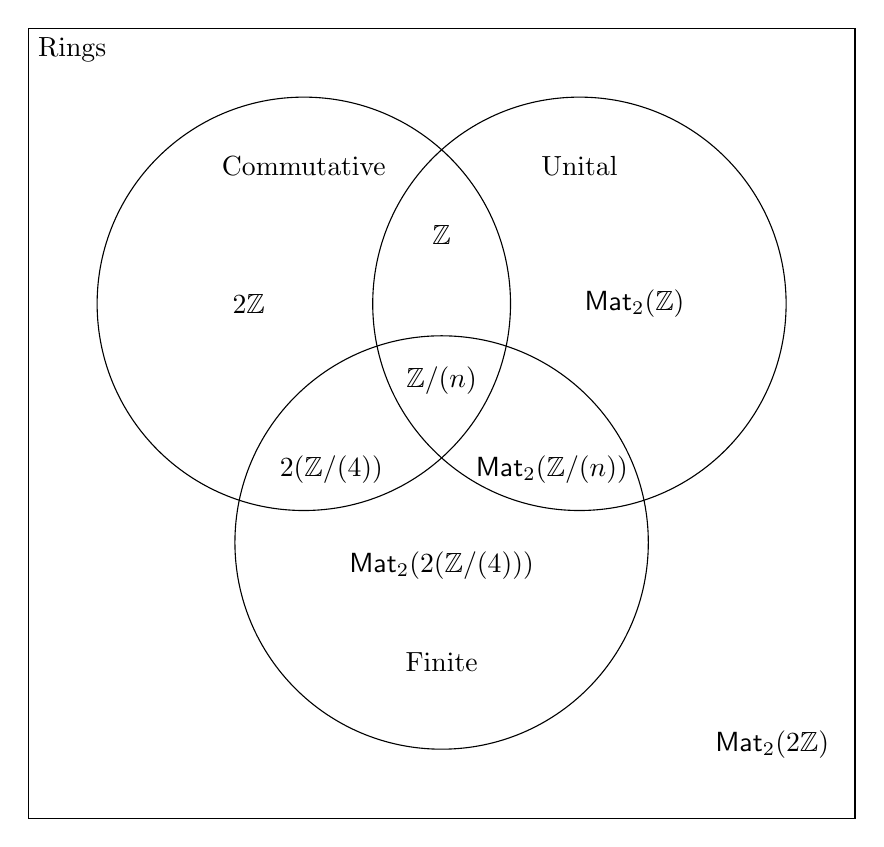
\begin{tikzpicture}[scale=0.35]
  \draw (-15,-18.66) -- (-15,10) -- (15,10) -- (15,-18.66) -- cycle;
  \draw (-5,0) circle (7.5);
  \draw (5,0) circle (7.5);
  \draw (0,-8.66) circle (7.5);
  \draw (-15,10) node [anchor=north west] {Rings};
  \draw (-5,5) node [anchor=center] {Commutative};
  \draw (5,5) node [anchor=center] {Unital};
  \draw (0,-13) node [anchor=center] {Finite};
  \draw (0,2.5) node [anchor=center] {\(\ZZ\)};
  \draw (0,-2.8) node [anchor=center] {\(\ZZ/(n)\)};
  \draw (-7,0) node [anchor=center] {\(2\ZZ\)};
  \draw (7,0) node [anchor=center] {\(\MAT{2}{\ZZ}\)};
  \draw (12,-16) node [anchor=center] {\(\MAT{2}{2\ZZ}\)};
  \draw (4,-6) node [anchor=center] {\(\MAT{2}{\ZZ/(n)}\)};
  \draw (-4,-6) node [anchor=center] {\(2(\ZZ/(4))\)};
  \draw (0,-9.5) node [anchor=center] {\(\MAT{2}{2(\ZZ/(4))}\)};
\end{tikzpicture}
\caption{\label{fig:ring-venn} A Venn diagram of ring families.}
\end{center}
\end{figure}



%---------%
\Exercises%
%---------%

\begin{exercise}
Show that \(\ZZ/(n)\) is a finite, commutative, unital ring for all \(n \geq 2\).
\end{exercise}


\begin{exercise}
Let \(X\) be a nonempty set.
\begin{proplist*}
\item Show that \(\POW{X}\) is commutative and unital, and that \(\POW{X}\) is finite if and only if \(X\) is finite.
\item Show that \(\POWP{X}\) is commutative and \emph{not} unital, and that \(\POWP{X}\) is finite if and only if \(X\) is finite.
\end{proplist*}
\end{exercise}


\begin{exercise}
Draw the cayley tables of the following rings.
This will be tedious.
\begin{proplist*}
\item \(\ZZ/(7)\)
\item \(\POWP{\{a,b\}}\)
\item \(\ZZ/(8)\)
\item \(\POW{\{a,b\}}\)
\item \(aR\), where \(R = \ZZ/(4)\) and \(a = [2]\)
\end{proplist*}
\end{exercise}


\begin{exercise}
Let \(R\) be a ring.
\begin{proplist}
\item Show that \(\MAT{2}{R}\) is unital if and only if \(R\) is unital.
\item Show that \(\MAT{2}{R}\) is finite if and only if \(R\) is finite.
\item Show that if \(R\) is not the zero ring, then \(\MAT{2}{R}\) is not commutative.
(Hint: find two specific matrices \(A\) and \(B\) such that \(AB \neq BA\).)
\end{proplist}
\end{exercise}


\begin{exercise}
Let \(R\) be a ring and \(A\) a nonempty set.
\begin{proplist}
\item Show that \(R^A\) is commutative if and only if \(R\) is commutative.
\item Show that \(R^A\) is unital if and only if \(R\) is unital.
\end{proplist}
\end{exercise}

\begin{exercise}
Show that the ring \(k\ZZ\), with \(k \geq 2\), is a commutative ring which is not unital.
(cf. \eref{exerc:aR-is-ring}.)
\end{exercise}


\begin{exercise}
If \(R\) is a unital ring, we can extend the power function \(a^\ast\) (cf. \ref{dfn:pow-elt}) to zero exponents by defining \(a^0 = 1_R\).
Show that if \(R\) is a unital ring, then the following properties hold for all \(a \in R\) and \(m,n \in \NN\).
\begin{proplist*}
\item \(a^{m+n} = a^m a^n\).
\item \(a^{mn} = (a^m)^n\).
\end{proplist*}
\end{exercise}


\begin{exercise}
Show that if \(R\) is commutative, then \((ab)^n = a^n b^n\) for all \(a,b \in R\) and all \(n \geq 1\).
If \(R\) is unital, show that this identity also holds for the case \(n = 0\).
\end{exercise}


\begin{exercise}[Binomial Theorem.] \label{exerc:binomial-theorem}
Let \(R\) be a commutative ring and let \(a,b \in R\).
Show that for all natural numbers \(n \geq 1\) we have \[ (a+b)^n = \sum_{k=0}^n {n \choose k} a^k b^{n-k}. \]
If \(R\) is unital, show that this identity also holds for the case \(n = 0\).
\end{exercise}


\begin{exercise}
Let \(R\) be a unital ring.
\begin{proplist*}
\item Suppose \(n1_R = 0_R\) for some \(n \geq 2\).
Show that \(\CHAR{R}\) divides \(n\).
\item Show that \(\CHAR{R} = \ADDORD{1_R}\).
\end{proplist*}
\end{exercise}


\begin{exercise}
Show that every finite ring has positive characteristic.
\end{exercise}


\begin{exercise}
Let \(R\) be a null ring.
\begin{proplist*}
\item Show that \(R\) is commutative.
\item Show that \(R\) is not unital.
\end{proplist*}
\end{exercise}


\begin{exercise}
Show that every boolean ring is commutative.
(Hint: Meditate upon \((a+b)^2\).)
\end{exercise}


\begin{exercise}
Exhibit a boolean ring which is unital, and another which is not unital.
\end{exercise}

      \newpage

    \section{Homomorphisms}
      \label{sec:ring-homs}
      The ring axioms represent a kind of abstract \emph{structure}. When two objects have the same kind of structure the \emph{structure-preserving mappings} between them are often useful. For example, consider the ring \(\ZZ/(5)\) of integers mod 5. As a set, \(\ZZ/(5)\) contains five equivalence classes of integers. We have a natural mapping \(\pi : \ZZ \rightarrow \ZZ/(5)\), namely the mapping that sends an integer \(k\) to its remainder (equivalence class) mod 5. Importantly this mapping respects the arithmetic on \(\ZZ\) in the sense that \(\pi(a+b) = \pi(a) + \pi(b)\) and \(\pi(ab) = \pi(a)\pi(b)\) -- the sum (product) of residues is the residue of the sum (product). This mapping can be used to show, for instance, that the equation \(a^4 + b^4 + c^4 = 4d^4\) has no nontrivial solutions in \(\ZZ\) by transporting any such solution to the finite ring \(\ZZ/(5)\). And so, we formalize the notion of ``structure-preserving map'' as follows.

\begin{dfn}[Ring Homomorphism] \label{dfn:ring-hom}
Let \(R\) and \(S\) be rings. A mapping \(\varphi : R \rightarrow S\) is called a \emph{ring homomorphism} if the following are satisfied. \index{homomorphism}
\begin{proplist}
\item \(\varphi(a + b) = \varphi(a) + \varphi(b)\) for all \(a,b \in R\).
\item \(\varphi(ab) = \varphi(a)\varphi(b)\) for all \(a,b \in R\).
\end{proplist}
If \(R\) and \(S\) are both unital rings, we say that \(\varphi\) is \emph{unital} if, in addition to the above, \(\varphi(1_R) = 1_S\). \index{unital!homomorphism}
\end{dfn}

A homomorphism \(\varphi : R \rightarrow S\) ``transports'' the structure of \(R\) into \(S\); in a concrete sense there is a ``shadow'' of \(R\) inside \(S\). If \(R\) and \(S\) are both unital rings, then the one element is an extra bit of structure which may be preserved.

\begin{prop} \mbox{} \label{prop:ring-cat}
\begin{proplist}
\item If \(R\) is a ring, then the \emph{identity map} \(\ID[R] : R \rightarrow R\) given by \(\ID[R](x) = x\) is a ring homomorphism. If \(R\) is unital, then \(\ID\) is unital. \label{prop:ring-cat:id}
\item If \(\varphi : R \rightarrow S\) and \(\psi : S \rightarrow T\) are ring homomorphisms, then the \emph{composite map} \(\psi \circ \varphi : R \rightarrow T\) is a homomorphism. If \(\varphi\) and \(\psi\) are unital, then \(\psi \circ \varphi\) is unital. \label{prop:ring-cat:comp}
\end{proplist}
\end{prop}

\begin{proof}
\begin{inlineproplist}
\item Letting \(x,y \in R\), we have \(\ID[R](x+y) = x+y = \ID[R](x) + \ID[R](y)\) and likewise \(\ID[R](xy) = xy = \ID[R](x)\ID[R](y)\), so that \(\ID[R]\) is a ring homomorphism. If \(R\) is unital, then \(\ID[R](1_R) = 1_R\) by definition.
\item Let \(x,y \in R\). We have
\begin{eqnarray*}
(\psi \circ \varphi)(x+y)
 & = & \psi(\varphi(x+y)) \\
 & = & \psi(\varphi(x) + \varphi(y)) \\
 & = & \psi(\varphi(x)) + \psi(\varphi(y)) \\
 & = & (\psi \circ \varphi)(x) + (\psi \circ \varphi)(y)
\end{eqnarray*}
so that \(\psi \circ \varphi\) preserves plus. Similarly, \((\psi \circ \varphi)(xy) = (\psi \circ \varphi)(x)(\psi \circ \varphi)(y)\) for all \(x,y \in R\), so that \(\psi \circ \varphi\) preserves times. Finally, if \(\varphi\) and \(\psi\) are unital, we have \((\psi \circ \varphi)(1_R) = \psi(\varphi(1_R)) = \psi(1_S) = 1_T\), thus \(\psi \circ \varphi\) is unital.
\end{inlineproplist}
\end{proof}

Although by definition a homomorphism preserves only plus and times, we can show that the zero and negation are also preserved.

\begin{prop} \label{prop:ring-hom-basics}
If \(\varphi : R \rightarrow S\) is a ring homomorphism, then we have the following.
\begin{proplist}
\item \(\varphi(0_R) = 0_S\). \label{prop:ring-hom-basics:zero}
\item \(\varphi(-a) = -\varphi(a)\) for all \(r \in R\). \label{prop:ring-hom-basics:neg}
\item \(\varphi(a-b) = \varphi(a) - \varphi(b)\) for all \(a,b \in R\). \label{prop:ring-hom-basics:minus}
\end{proplist}
\end{prop}

\begin{proof}
\begin{inlineproplist}
\item Note that \(\varphi(0_R) + \varphi(0_R) = \varphi(0_R + 0_R) = \varphi(0_R)\). By \sref{prop:ring-basics}{zero-unique}, we have \(\varphi(0_R) = 0_S\).
\item Note that \(\varphi(a) + \varphi(-a) = \varphi(a + (-a)) = \varphi(0_R) = 0_S\), using \ref{prop:ring-hom-basics:zero}. By \sref{prop:ring-basics}{negative-unique}, we have \(\varphi(-a) = -\varphi(a)\).
\item Follows from \ref{prop:ring-hom-basics:neg}.
\end{inlineproplist}
\end{proof}


\begin{examples}
\item The natural projection \(\pi : \ZZ \rightarrow \ZZ/(n)\) is a surjective unital ring homomorphism for any \(n\).

\item If \(R\) is any ring, then there is exactly one ring homomorphism \(\varphi : R \rightarrow 0\), and exactly one homomorphism \(\psi : 0 \rightarrow R\). Neither of these is ever unital.

\item Let \(R\) be any unital ring. Then \(\varphi : R \rightarrow \MAT{2}{R}\) given by \[ \varphi(r) = \begin{bmatrix} 0 & 0 \\ -r & r \end{bmatrix} \] is a ring homomorphism. Although \(R\) (and hence \(\MAT{2}{R}\)) is unital, \(\varphi\) is \emph{not} a unital homomorphism. (Why?)
\end{examples}

When studying algebra, it is often the case that we are concerned with several objects at once along with some of the homomorphisms among them. In this case we can make our lives easier by using a \emph{commutative diagram}. \index{commutative diagram} A \emph{diagram} is a collection of rings and homomorphisms among them, represented graphically using labeled arrows. For example, suppose we are concerned with rings \(A\), \(B\), \(C\), and \(D\), as well as homomorphisms \(\varphi : A \rightarrow B\), \(\psi : C \rightarrow D\), \(\chi : A \rightarrow C\), and \(\theta : B \rightarrow D\). We might represent these data using the following diagram.
\begin{center}
\begin{tikzcd}
A \arrow[r,"\varphi"] \arrow[d, "\chi"'] & B \arrow[d, "\theta"] \\
C \arrow[r, "\psi"']                     & D
\end{tikzcd}
\end{center}
The arrows are meant to suggest the flow of elements through a network of conduits. A diagram is said to \emph{commute} if any two composite chains of homomorphisms with the same start and end points are equal. For instance, the above diagram is commutative precisely when \(\theta \circ \varphi = \psi \circ \chi\). This is a powerful idea; when a diagram commutes we can prove things about mappings using substitution.

It turns out that lots of important theorems can be stated in the form ``there is a unique map which makes such-and-such diagram commute''. It also turns out that, once we get used to thinking in terms of homomorphisms, this can be a powerful way to prove theorems. (Diagrams can also look pretty.) We will see several commutative diagrams in this text, but as an initial example, \ref{prop:ring-cat} can be understood to assert that the two diagrams in \autoref{fig:ring-cat-diagram} commute for any \(\varphi\) and \(\psi\). (Why?)
\begin{figure}[h!]
\begin{center}
\begin{tikzcd}
R \arrow[d, "\ID"'] \arrow[rd, "\varphi"] &   & & & R \arrow[dd, "\psi \circ \varphi"' description] \arrow[dr, "\varphi"] &   \\
R \arrow[r, "\varphi" description] \arrow[rd, "\varphi"'] & S \arrow[d, "\ID"] & & &   & S \arrow[ld, "\psi"] \\
  & S & & & T &
\end{tikzcd}
\caption{The punchline of \ref{prop:ring-cat}. \label{fig:ring-cat-diagram}}
\end{center}
\end{figure}



%---------%
\Exercises%
%---------%

\begin{exercise}
Show that the projection map \(\pi : \ZZ \rightarrow \ZZ/(n)\) given by \(\pi(k) = [k]\) is a unital ring homomorphism.
\end{exercise}

\begin{exercise}
Let \(\varphi : R \rightarrow S\) be a ring homomorphism.
\begin{proplist}
\item Show that \(\varphi(a^n) = \varphi(a)^n\) for all \(a \in R\) and all positive \(n\).
\item Show that \(\varphi(a^0) = \varphi(a)^0\) for all \(a \in R\) if and only if \(\varphi\) is unital.
\end{proplist}
\end{exercise}

\begin{exercise}
Show that if \(\varphi : R \rightarrow S\) is a homomorphism, then \[ \varphi\left( \sum_{i=a}^b r_i \right) = \sum_{i=a}^b \varphi(r_i) \] for all finite sequences \(r_i\).
\end{exercise}

\begin{exercise}
Let \(R\) and \(S\) be rings. Show that the map \(\varphi : R \rightarrow S\) given by \(\varphi(x) = 0_S\) for all \(x \in R\) is a ring homomorphism. Is this map ever unital?
\end{exercise}

If we wish to understand a ring, we must also understand the homomorphisms to and from that ring. The next three exercises characterize some of the homomorphisms involving $0$, $\ZZ$, and $\ZZ/(n)$.

\begin{exercise}[Homomorphisms to and from \(0\).]
Let \(R\) be a ring.
\begin{proplist*}
\item Show that there is a \emph{unique} ring homomorphism \(R \rightarrow 0\).
\item Show that there is a \emph{unique} ring homomorphism \(0 \rightarrow R\).
\end{proplist*}
\end{exercise}

\begin{exercise}[Homomorphisms from \(\ZZ\).] \label{exerc:homs-from-zz}
Let \(R\) be a ring.
\begin{proplist}
\item Let \(\varphi : \ZZ \rightarrow R\) be a ring homomorphism. Show that \(\varphi\) is uniquely determined by its image at \(1\) in the following sense: if \(\psi\) is another ring homomorphism \(\ZZ \rightarrow R\) such that \(\psi(1) = \varphi(1)\), then \(\psi = \varphi\).
\item Let \(a \in R\) be a fixed element. Show that there exists a ring homomorphism \(\varphi : \ZZ \rightarrow R\) such that \(\varphi(1) = a\). (Hint: there's only one way to do it.)
\item Show that if \(R\) is unital, then there is a \emph{unique} unital ring homomorphism \(\ZZ \rightarrow R\).
\end{proplist}
\end{exercise}

\begin{exercise}[Homomorphisms from \(\ZZ/(n)\).] \label{exerc:homs-from-zzn}
Let \(n \geq 2\) be a positive integer and let \(R\) be a ring.
\begin{proplist}
\item Show that every ring homomorphism \(\varphi : \ZZ/(n) \rightarrow R\) is uniquely determined by its image of \(1\) in the following sense: if \(\psi\) is another ring homomorphism \(\ZZ/(n) \rightarrow R\) such that \(\psi(1) = \varphi(1)\), then \(\psi = \varphi\).
\item Let \(a \in R\) be a fixed element. Show that there exists a ring homomorphism \(\varphi : \ZZ/(n) \rightarrow R\) such that \(\varphi(1) = a\) if and only if \(a\) is annihilated by a divisor of \(n\). Take care that your map is well-defined. (Hint: there's only one way to do it.)
\item Show that if \(R\) is unital and \(\CHAR{R}\) divides \(n\), then there is a \emph{unique} unital ring homomorphism \(\ZZ/(n) \rightarrow R\).
\end{proplist}
\end{exercise}

\begin{exercise}
Show that if \(\varphi : R \rightarrow S\) is a unital ring homomorphism, then \(\CHAR{S}\) divides \(\CHAR{R}\). (@@@)
\end{exercise}

\begin{exercise}
Let \(R\) be a commutative ring and \(e \in R\) idempotent. Show that the ``multiplication map'' \(\mu_e : R \rightarrow R\) given by \(\mu_e(x) = ex\) is a ring homomorphism. If \(R\) is also unital, is \(\mu_e\) ever unital? (@@@)
\end{exercise}

\begin{exercise}
Let \(A\) be a nonempty set, with \(a \in A\) a fixed element, and let \(R\) be a ring. Show that the \emph{evaluation map} \(\varepsilon_a : R^A \rightarrow R\) given by \(\varepsilon_a(f) = f(a)\) is a ring homomorphism. Show that if \(R\) is a unital ring, then \(\varepsilon_a\) is a unital homomorphism.
\end{exercise}

\begin{exercise}
Let \(\varphi : R \rightarrow S\) be a ring homomorphism and let \(a \in R\).
\begin{proplist}
\item Show that if \(a\) is idempotent, then \(\varphi(a)\) is idempotent, but the converse does not hold.
\item Show that if \(a\) is nilpotent, then \(\varphi(a)\) is nilpotent, but the converse does not hold.
\end{proplist}
\end{exercise}

\begin{exercise}
Let \(X\) and \(Y\) be sets and \(f : X \rightarrow Y\) an injective map. Denote by \(\Phi_f\) the induced map \(\POW{X} \rightarrow \POW{Y}\) given by \(\Phi_f(A) = f[A]\).
\begin{proplist}
\item Show that \(\Phi_f\) is a ring homomorphism.
\item Show that \(\Phi_f\) is unital if and only if \(f\) is surjective.
\end{proplist}
\end{exercise}

\begin{dfn}[Endomorphism] \label{dfn:endo}
Let \(R\) be a ring. A ring homomorphism \(R \rightarrow R\) is called an \index{endomorphism} \emph{endomorphism}. We denote by \(\END{R}\) the set of all ring endomorphisms of \(R\), and by \(\ENDU{R}\) the set of all \emph{unital} ring endomorphisms of \(R\). Certainly we have \(\ENDU{R} \subseteq \END{R}\), and neither set is empty, since \(\ID[R]\) is a unital endomorphism.
\end{dfn}

\begin{exercise}[Endomorphism Arithmetic.]
Given a ring \(R\), the set \(\END{R}\) comes with a sort of arithmetic. We define the sum of two endos pointwise, and the product of two endos by composition.
\begin{proplist}
\item Show that if \(\alpha, \beta \in \END{R}\), then \(\alpha\beta \in \END{R}\).
\item Show that if \(\alpha, \beta \in \END{R}\), then \(\alpha + \beta\) need not be in \(\END{R}\). (Give an example.)
\item Show that if \(\alpha, \beta \in \ENDU{R}\), then \(\alpha + \beta\) is not in \(\ENDU{R}\).
\end{proplist}
\end{exercise}

\begin{exercise}
Show that if \(R\) is a null ring, then \(\END{R}\) is a ring. (It turns out that this ring is extremely important.)
\end{exercise}

(@@@) characterize the homomorphisms \(\ZZ/(m) \rightarrow \ZZ/(n)\).

      \newpage

    \section{Direct Sums}
      \label{sec:direct-sums}
      How do we find concrete examples of rings? Most sets don't have obvious choices for the plus and times operations lying around. But if we have some \emph{existing} rings, equipped with plus and times, we might hope to use that existing arithmetic to construct a new one. So a major motivating question throughout this text is what we will call
\begin{titlebox}{The Construction Problem}
\begin{center}
How can we build new rings out of the ``parts'' of old ones?
\end{center}
\end{titlebox}
We will see that, while this question is nebulous enough to avoid a complete answer, there are many useful partial answers. The first, and perhaps the simplest, is to construct \emph{direct sums}: two (or more) rings glued together as a cartesian product.

\begin{dfn}[Direct Sum of Two Rings] \label{dfn:direct-sum}
Let \(R\) and \(S\) be rings. Then the \emph{direct sum} \index{direct sum} of \(R\) and \(S\), denoted \(R \oplus S\), is the cartesian product \[ R \oplus S = \{ (r,s) \mid r \in R, s \in S \} \] equipped with the ``componentwise'' operations defined as follows.
\begin{eqnarray*}
(r_1, s_1) + (r_2, s_2) & = & (r_1 + r_2, s_1 + s_2) \\
(r_1, s_1) \cdot (r_2, s_2) & = & (r_1 \cdot r_2, s_1 \cdot s_2)
\end{eqnarray*}
\end{dfn}

The cartesian product is one of the least sophisticated ways to bolt two sets together, and the least sophisticated way to attempt a ring structure on a cartesian product is to perform arithmetic coordinatewise. Of course we have to verify that these operations make \(R \oplus S\) into a ring; the proof of this is left to the exercises.

\begin{prop} \label{prop:direct-sum}
Given rings \(R\) and \(S\) we have the following.
\begin{proplist}
\item The direct sum \(R \oplus S\) with the componentwise operations is a ring.
\item The \emph{coordinate projections} \(\pi_1 : R \oplus S \rightarrow R\) and \(\pi_2 : R \oplus S \rightarrow S\), given by \(\pi_1(r,s) = r\) and \(\pi_2(r,s) = s\), are surjective ring homomorphisms.
\item The \emph{coordinate injections} \(\iota_1 : R \rightarrow R \oplus S\) and \(\iota_2 : S \rightarrow R \oplus S\), given by \(\iota_1(r) = (r,0_S)\) and \(\iota_2(s) = (0_R,s)\), are injective ring homomorphisms.
\end{proplist}
\end{prop}

Although (or perhaps because) the direct sum is such a simple way to build new rings out of old ones, it is a very important tool in our quest to understand the structure of rings. We also get some mappings for free, the coordinate projections \(\pi_1\) and \(\pi_2\) and injections \(\iota_1\) and \(\iota_2\). These mappings are simple, but they play a very important structural role for the direct sum.

\begin{examples}
\item The ring \(\ZZ \oplus \ZZ\) is, as a set, \[ \ZZ \oplus \ZZ = \{ (a,b) \mid a,b \in \ZZ \}. \] In this ring we have, for example, \[ (1,2) + (4,-3) = (1+4, 2-3) = (5,-1) \] and \[ (2,-1) \cdot (5,0) = (2 \cdot 5, -1 \cdot 0) = (10,0). \]
\item The ring \(\ZZ/(2) \oplus \ZZ/(2)\) has 4 elements. The cayley table of this ring is shown in \autoref{fig:cayley-zz2pzz2}.
\begin{figure}[h!]
\begin{center}
\small
\addtolength{\tabcolsep}{-2pt}
\begin{tabular}{c|cccc}
\(+\) & (0,0) & (0,1) & (1,0) & (1,1) \\ \hline
(0,0) & (0,0) & (0,1) & (1,0) & (1,1) \\
(0,1) & (0,1) & (0,0) & (1,1) & (1,0) \\
(1,0) & (1,0) & (1,1) & (0,0) & (0,1) \\
(1,1) & (1,1) & (1,0) & (0,1) & (0,0)
\end{tabular}
\quad
\begin{tabular}{c|cccc} \setlength{\tabcolsep}{5pt}
\(\cdot\)
      & (0,0) & (0,1) & (1,0) & (1,1) \\ \hline
(0,0) & (0,0) & (0,0) & (0,0) & (0,0) \\
(0,1) & (0,0) & (0,1) & (0,0) & (0,1) \\
(1,0) & (0,0) & (0,0) & (1,0) & (1,0) \\
(1,1) & (0,0) & (0,1) & (1,0) & (1,1)
\end{tabular}
\addtolength{\tabcolsep}{2pt}
\end{center}
\caption{Cayley tables of \(\ZZ/(2) \oplus \ZZ/(2)\).\label{fig:cayley-zz2pzz2}}
\end{figure}
\end{examples}

We can think of \(\oplus\) like an operation on \emph{rings}, which takes two rings and builds a new one. It isn't an operation quite like plus on \(\ZZ\), though, because operations can only be defined on \emph{sets}, but there is no set of all rings. But it is still reasonable to hope that as an operation-like thing, \(\oplus\) behaves nicely. For instance, we might hope that for two rings \(R\) and \(S\), we have \(R \oplus S = S \oplus R\). Of course this cannot possibly be true; as sets, \(R \oplus S\) and \(S \oplus R\) will generally be disjoint. In the next section, we will see how to get around this restriction.

There are other ways to put a ring structure on a cartesian product of rings; some of these are explored in the exercises, and another is in \autoref{sec:quad-ext}.



%---------%
\Exercises%
%---------%

\begin{exercise}
Construct the cayley tables of the following rings.
\begin{proplist*}
\item \(\ZZ/(2) \oplus \ZZ/(2)\)
\item \(\ZZ/(2) \oplus \ZZ/(3)\)
\item \(2R \oplus \ZZ/(3)\), where \(R = \ZZ/(4)\)
\end{proplist*}
\end{exercise}

\begin{exercise}
Let \(R\) and \(S\) be rings.
\begin{proplist*}
\item Show that \(R \oplus S\) is commutative if and only if \(R\) and \(S\) are commutative.
\item Show that \(R \oplus S\) is boolean if and only if \(R\) and \(S\) are boolean.
\item Show that \(R \oplus S\) is unital if and only if \(R\) and \(S\) are unital, and in this case \(1_{R \oplus S} = (1_R, 1_S)\).
\item Show that \(R \oplus S\) is null if and only if \(R\) and \(S\) are null.
\item Show that \(R \oplus S\) is finite if and only if \(R\) and \(S\) are finite.
\end{proplist*}
\end{exercise}

\begin{exercise}
Show that if \(R\) is unital, then the coordinate projection \(\pi_1 : R \oplus S \rightarrow R\) is a unital homomorphism.
\end{exercise}

\begin{exercise}
Prove \propref{prop:direct-sum}.
\end{exercise}

\begin{exercise}
Let \(R\) and \(S\) be rings and let \((r,s) \in R \oplus S\).
\begin{proplist}
\item Show that \((r,s)^n = (r^n, s^n)\) for all \(n \in \NN \setminus \{0\}\). (cf. \eref{exerc:ring-powers})
\item If \(R\) and \(S\) are both unital, show that this identity also holds for \(n = 0\).
\end{proplist}
\end{exercise}

\begin{exercise}
Let \(R\) and \(S\) be rings and let \((r,s) \in R \oplus S\). Show that \(n(r,s) = (nr, ns)\) for all \(n \in \ZZ\). (cf. \eref{exerc:elt-mult})
\end{exercise}

\begin{exercise}
Show that \(\CHAR{R \oplus S} = \LCM{\CHAR{R}}{\CHAR{S}}\).
\end{exercise}

\begin{exercise}[Universal Property of Binary Direct Sums.] \label{exerc:up-direct-sum} \index{universal property!of direct sums}
Let \(R\), \(S\), and \(T\) be rings. Suppose we have ring homomorphisms \(\varphi : T \rightarrow R\) and \(\psi : T \rightarrow S\). Then there is a unique ring homomorphism \(\Theta : T \rightarrow R \oplus S\) such that the following diagram commutes.
\begin{center}
\begin{tikzcd}
 & T \arrow[ld,"\varphi"'] \arrow[rd, "\psi"] \arrow[d, dashed, "\Theta"] & \\
R & R \oplus S \arrow[l,"\pi_1"] \arrow[r, "\pi_2"'] & S
\end{tikzcd}
\end{center}
That is, there is a unique \(\Theta\) such that \(\pi_1 \circ \Theta = \varphi\) and \(\pi_2 \circ \Theta = \psi\).
\end{exercise}

Before we give the proof of this result, a note on its importance. The punchline of \eref{exerc:up-direct-sum} asserts the existence of a unique homomorphism \(\Theta\) through which any pair \((\varphi, \psi)\) must ``factor through''. This is the first of several results about rings known as \emph{universal properties}. The precise meaning of the term ``universal property'' is not important for us at the moment; it is enough to think of them as giving us ``unique homomorphisms for free'', in this case, homomorphisms into a direct sum. They usually also involve a kind of unique factorization of homomorphisms as we have here.

\begin{exercise}
When is the induced map in UPDP unital?
\end{exercise}

\begin{exercise}
Let \(R\), \(S\), and \(T\) be rings with homomorphisms \(\varphi : T \rightarrow R\) and \(\psi : T \rightarrow S\). Show that if \(\varphi\) and \(\psi\) are both injective, then the induced map \(\Theta : T \rightarrow R \oplus S\) is injective.
\end{exercise}

\begin{exercise}
Let \(\varphi : R_1 \rightarrow R_2\) and \(\psi : S_1 \rightarrow S_2\) be ring homomorphisms.
\begin{proplist}
\item Show that the mapping \(\Theta : R_1 \oplus S_1 \rightarrow R_2 \oplus S_2\) given by \(\Theta(r,s) = (\varphi(r), \psi(s))\) is a homomorphism. We refer to this mapping as \(\varphi \oplus \psi\).
\item (@@@) surjective
\item (@@@) injective
\item (@@@) unital
\end{proplist}
\end{exercise}

\begin{exercise}[A Zero-Square Ring.]
The componentwise operations are not the only way to turn the setwise cartesian product of rings into a ring. Here is another. Let \(S\) be a commutative ring and let \(R = S \times S \times S\). Define addition on \(R\) componentwise, and define multiplication by \[ (a_1,a_2,a_3) \cdot (b_1,b_2,b_3) = (0,0,a_1b_2 - a_2b_1). \] Show that \(R\) is a ring, and that \(x^2 = 0\) for all \(x \in R\).
\end{exercise}

\begin{exercise}
(@@@) move to subrings \textbf{Direct Products.} Let \(\Lambda\) be a nonempty set and let \(\mathcal{R} = \{ R_i \mid i \in \Lambda \}\) be a family of rings indexed by \(\Lambda\). We denote by \[ \prod_{i \in \Lambda} R_i \] the set of all mappings \(r : \Lambda \rightarrow \bigcup_{i \in \Lambda} R_i\) such that \(r(i) \in R_i\) for all \(i \in \Lambda\).
\begin{proplist}
\item Show that \(\prod_{i \in \Lambda} R_i\) is a ring with respect to pointwise plus and times.
\item Show that \(\prod_{i \in \Lambda} R_i\) is commutative if and only if \(R_i\) is commutative for each \(i \in \Lambda\).
\item Show that \(\prod_{i \in \Lambda} R_i\) is unital if and only if \(R_i\) is unital for each \(i \in \Lambda\).
\end{proplist}
\end{exercise}

\begin{exercise}
(@@@) move to subrings \textbf{Direct Sums.} Let \(\Lambda\) be a nonempty set and let \(\mathcal{R} = \{ R_i \mid i \in \Lambda \}\) be a family of rings indexed by \(\Lambda\). We say that an element \(\alpha \in \prod_{i \in \Lambda} R_i\) has \emph{finite support} if \(\alpha(i) = 0\) for all but finitely many \(i \in \Lambda\). We denote by \[ \bigoplus_{i \in \Lambda} R_i \] the set of all \(\alpha \in \prod_{i \in \Lambda} R_i\) of finite support.
\begin{proplist}
\item Show that \(\bigoplus_{i \in \Lambda} R_i\) is a subring of \(\prod_{i \in \Lambda} R_i\).
\item Show that \(\bigoplus_{i \in \Lambda} R_i\) is commutative if and only if \(R_i\) is commutative for each \(i \in \Lambda\).
\item Show that \(\bigoplus_{i \in \Lambda} R_i\) is unital if and only if \(R_i\) is unital for each \(i \in \Lambda\) and \(\Lambda\) is finite.
\end{proplist}
\end{exercise}

\begin{dfn}
Let \(R\) and \(S\) be rings, and let \(\theta : R \rightarrow \END{S}\) be a mapping. Note that \(\END{R}\) is not (generally) a ring under pointwise addition and composition, so \(\theta\) cannot possibly be a ring homomorphism. Instead, we say that \(\theta\) is a \emph{prehomomorphism} if \(\theta(a + b) = \theta(a) + \theta(b)\) and \(\theta(ab) = \theta(a)\theta(b)\) for all \(a,b \in R\). In this case, note that \(\IM{\theta}\) is a ring.

If \(\theta\) is a prehomomorphism such that \(\IM{theta}\) is commutative, we can define an alternative arithmetic on the cartesian product \(R \times S\) as follows. Addition is performed coordinatewise, while \[ (r_1, s_1) \cdot (r_2, s_2) = (r_1r_2, \theta(r_1)(s_2) + \theta(r_2)(s_1)). \] We call this the \emph{null extension} of \(S\) by \(R\) via \(\theta\), denoted \(\REXTEND{R}{\theta}{S}\)
\end{dfn}

\begin{exercise}
Show that \(\REXTEND{R}{\theta}{S}\) is a ring.
\end{exercise}

\begin{exercise}
Let \(S\) be a ring.
\begin{proplist}
\item Show that the map \(\theta : 0 \rightarrow \END{S}\) given by \(\theta(0)(s) = 0_S\) is a prehomomorphism, and that \(\IM{\theta}\) is commutative.
\item Show that \(\REXTEND{0}{\theta}{S}\) is a null ring, which has the same additive structure as \(S\). We call this the \emph{nullification} of \(S\), and denote it \(S^0\).
\end{proplist}
\end{exercise}

\begin{exercise}
Let \(R\) be a ring and \(N\) a null ring, and suppose we have a prehomomorphism \(\theta\) with \(\IM{\theta}\) commutative.
\end{exercise}

\begin{exercise}
Let \(R\) be a commutative ring. We define operations on the set \(\HAM{R} = R \times R \times R \times R\) by (@@@)
\begin{proplist}
\item These operations make \(\HAM{R}\) a noncommutative ring.
\item The map \(\iota : R \rightarrow \HAM{R}\) given by \(\iota(r) = (r,0,0,0)\) is an injective ring homomorphism.
\item If \(R\) is a field, then \(\HAM{R}\) is a skew field.
\end{proplist}
\end{exercise}

      \newpage

    \section{Isomorphisms}
      \label{sec:ring-isos}
      Just for fun, let's consider the cayley tables of the ring \(\ZZ/(6)\) as shown in \autoref{fig:cayley-zz6}.
\begin{figure}[h!]
\begin{center}
\begin{tabular}{c|cccccc}
\(+\)
  & 0 & 1 & 2 & 3 & 4 & 5 \\ \hline
0 & 0 & 1 & 2 & 3 & 4 & 5 \\
1 & 1 & 2 & 3 & 4 & 5 & 0 \\
2 & 2 & 3 & 4 & 5 & 0 & 1 \\
3 & 3 & 4 & 5 & 0 & 1 & 2 \\
4 & 4 & 5 & 0 & 1 & 2 & 3 \\
5 & 5 & 0 & 1 & 2 & 3 & 4
\end{tabular}
\quad\quad
\begin{tabular}{c|cccccc}
\(\cdot\)
  & 0 & 1 & 2 & 3 & 4 & 5\\ \hline
0 & 0 & 0 & 0 & 0 & 0 & 0 \\
1 & 0 & 1 & 2 & 3 & 4 & 5 \\
2 & 0 & 2 & 4 & 0 & 2 & 4 \\
3 & 0 & 3 & 0 & 3 & 0 & 3 \\
4 & 0 & 4 & 2 & 0 & 4 & 2 \\
5 & 0 & 5 & 4 & 3 & 2 & 1 \\
\end{tabular}
\caption{\label{fig:cayley-zz6} Cayley tables of \(\ZZ/(6)\).}
\end{center}
\end{figure}
Let's also consider the cayley tables of the ring \(\ZZ/(2) \oplus \ZZ/(3)\), with the row and column headings written in a particular order (which will be explained in a moment) as shown in \autoref{fig:cayley-zz2-zz3}.
Drawing these tables is a little tedious, but straightforward.
\begin{figure}[h!]
\begin{center}
\begin{tabular}{c|cccccc}
\(+\) & (0,0) & (1,1) & (0,2) & (1,0) & (0,1) & (1,2) \\ \hline
(0,0) & (0,0) & (1,1) & (0,2) & (1,0) & (0,1) & (1,2) \\
(1,1) & (1,1) & (0,2) & (1,0) & (0,1) & (1,2) & (0,0) \\
(0,2) & (0,2) & (1,0) & (0,1) & (1,2) & (0,0) & (1,1) \\
(1,0) & (1,0) & (0,1) & (1,2) & (0,0) & (1,1) & (0,2) \\
(0,1) & (0,1) & (1,2) & (0,0) & (1,1) & (0,2) & (1,0) \\
(1,2) & (1,2) & (0,0) & (1,1) & (0,2) & (1,0) & (0,1)
\end{tabular}

\vspace{0.5cm}

\begin{tabular}{c|cccccc}
\(\cdot\) & (0,0) & (1,1) & (0,2) & (1,0) & (0,1) & (1,2) \\ \hline
(0,0)     & (0,0) & (0,0) & (0,0) & (0,0) & (0,0) & (0,0) \\
(1,1)     & (0,0) & (1,1) & (0,2) & (1,0) & (0,1) & (1,2) \\
(0,2)     & (0,0) & (0,2) & (0,1) & (0,0) & (0,2) & (0,1) \\
(1,0)     & (0,0) & (1,0) & (0,0) & (1,0) & (0,0) & (1,0) \\
(0,1)     & (0,0) & (0,1) & (0,2) & (0,0) & (0,1) & (0,2) \\
(1,2)     & (0,0) & (1,2) & (0,1) & (1,0) & (0,2) & (1,1) \\
\end{tabular}
\caption{\label{fig:cayley-zz2-zz3} Cayley tables of \(\ZZ/(2) \oplus \ZZ/(3)\).}
\end{center}
\end{figure}
It may be tricky to spot at first, but these two pairs of cayley tables are \emph{essentially the same}.
Why?
Note that the only real difference between the addition tables for \(\ZZ/(6)\) and \(\ZZ/(2) \oplus \ZZ/(3)\) is the \textbf{labels of the elements}.
Specifically, we can relabel them as follows.
\begin{center}
\begin{tabular}{ccc}
\(0 \leftrightarrow (0,0)\) & \(1 \leftrightarrow (1,1)\) & \(2 \leftrightarrow (0,2)\) \\
\(3 \leftrightarrow (1,0)\) & \(4 \leftrightarrow (0,1)\) & \(5 \leftrightarrow (1,2)\)
\end{tabular}
\end{center}
The same is true of the multiplication tables.
It may help to draw these cayley tables in color, so that corresponding elements are the same color.
Thinking of this correspondence between \(\ZZ/(6)\) and \(\ZZ/(2) \oplus \ZZ/(3)\) as a mapping, the sameness of the cayley tables gives us a little more: the correspondence is a \emph{homomorphism}.

Note that we can arrange the row and column labels of \autoref{fig:cayley-zz6} and \autoref{fig:cayley-zz2-zz3} however we like, but using this particular ordering makes it easier to see the correspondence.
Changing the order does not destroy the correspondence, it only makes it harder to see.

This relabeling raises an interesting question: in what sense are \(\ZZ/(6)\) and \(\ZZ/(2) \oplus \ZZ/(3)\) different rings?
Of course they are different as \emph{sets}.
But from a ring-theoretic perspective we only really care about \emph{structure} -- that is, the arithmetic, as embodied in the cayley tables.
These two rings have exactly the same structure, and we can translate between them via the relabeling without losing any information.
So in a sense \(\ZZ/(6)\) and \(\ZZ/(2) \oplus \ZZ/(3)\) are really two different manifestations of the same abstract ring structure, obtained by giving the elements different names.
When two rings are related in this way, we say they are \emph{isomorphic} to one another.

\begin{dfn} \label{dfn:isomorphism}
Let \(R\) and \(S\) be rings and \(\varphi : R \rightarrow S\) a ring homomorphism.
If \(\varphi\) is also bijective as a mapping, we say \(\varphi\) is an \emph{isomorphism}\index{isomorphism}.
In this case we say that \(R\) is \emph{isomorphic to} \(S\), denoted \(R \cong S\).
\end{dfn}

Remember: to show that one ring is isomorphic to another, we must find a bijective homomorphism from one to the other.
Conversely, if we know in advance that \(R \cong S\), then \emph{there exists} an isomorphism \(R \rightarrow S\); in general there may be many such mappings.
Isomorphisms formalize and generalize the ``structure preserving relabeling'' we saw between \(\ZZ/(6)\) and \(\ZZ/(2) \oplus \ZZ/(3)\).
In a very concrete sense, if \(R \cong S\), then \(R\) and \(S\) are really ``the same'' ring.
\emph{Isomorphism is structural equality.}
It is not too surprising, then, that ``is isomorphic to'' behaves very much like equality.

\begin{prop} \label{prop:iso-equiv}
For all rings \(R\), \(S\), and \(T\), the following hold.
\begin{proplist*}
\item \label{prop:iso-equiv:refl} \(R \cong R\).
\item \label{prop:iso-equiv:symm} If \(R \cong S\) then \(S \cong R\).
\item \label{prop:iso-equiv:trans} If \(R \cong S\) and \(S \cong T\) then \(R \cong T\).
\end{proplist*}
\end{prop}

A note before we prove this result: \ref{prop:iso-equiv} appears to be saying that \(\cong\) is an equivalence relation.
We have to be careful here, though, because equivalence relations only exist \emph{on sets}.
There is no set of all rings, for the same reason that there is no set of all sets.
And so we cannot say that isomorphism ``is'' an equivalence relation, even though it ``acts like'' and equivalence relation.

\begin{proof}
\begin{inlineproplist}
\item The identity mapping \(\ID : R \rightarrow R\) is a bijective homomorphism by \sref{prop:ring-cat}{id}.
\item Suppose we have an isomorphism \(\varphi : R \rightarrow S\).
Since \(\varphi\) is a bijection, it has an inverse \(\varphi^{-1} : S \rightarrow R\), with the property that \(\varphi \circ \varphi^{-1} = \ID[S]\) and \(\varphi \circ \varphi^{-1} = \ID[R]\) and which is also a bijection.
It thus suffices to show that \(\varphi^{-1}\) is also a ring homomorphism.
To this end, let \(x,y \in S\).
We then have the following.
\begin{eqnarray*}
\varphi^{-1}(x + y) & = & \varphi^{-1}\left(\ID[S](x) + \ID[S](y)\right) \\
 & = & \varphi^{-1}\left( (\varphi \circ \varphi^{-1})(x) + (\varphi \circ \varphi^{-1})(y) \right) \\
 & = & \varphi^{-1}\left( \varphi(\varphi^{-1}(x)) + \varphi(\varphi^{-1}(y)) \right) \\
 & = & \varphi^{-1}\left( \varphi\left( \varphi^{-1}(x) + \varphi^{-1}(y) \right) \right) \\
 & = & (\varphi^{-1} \circ \varphi)\left( \varphi^{-1}(x) + \varphi^{-1}(y) \right) \\
 & = & \ID[R]\left( \varphi^{-1}(x) + \varphi^{-1}(y) \right) \\
 & = & \varphi^{-1}(x) + \varphi^{-1}(y).
\end{eqnarray*}
Thus \(\varphi^{-1}\) preserves plus.
A similar argument shows that \(\varphi^{-1}\) preserves times, and so \(\varphi^{-1}\) is a ring homomorphism.
\item If \(R \cong S\) and \(S \cong T\), then we have bijective homomorphisms \(\varphi : R \rightarrow S\) and \(\psi : S \rightarrow T\).
Now \(\psi \circ \varphi : R \rightarrow T\) is a homomorphism by \sref{prop:ring-cat}{comp}, and since the composite of bijections is bijective, \(\psi \circ \varphi\) is bijective.
Thus \(R \cong T\).
\end{inlineproplist}
\end{proof}

Given two mathematical objects, one of the most basic questions we can ask about them is whether or not they are the same.
To emphasize the importance of this question, we'll give it a fancy name.

\begin{titlebox}{The Distinction Problem}
\begin{center}
Given rings \(R\) and \(S\), can we detect whether or not \(R \cong S\)?
\end{center}
\end{titlebox}

The Distinction Problem is one of the big questions of algebra.
Big enough, in fact, that we cannot hope for a complete answer; the best we can hope for is a sequence of partial answers of increasing power and sophistication.
To this end it is useful to have on hand several properties of rings which are \emph{preserved} by isomorphisms, so that two rings which differ must be nonisomorphic.
For instance, the property ``contains the number 3 as an element'' \emph{is not} preserved by isomorphisms: the elements of isomorphic rings may have nothing to do with each other.
However, the property ``consists of three elements'' \emph{is} preserved by isomorphisms.
Here are some others.

\begin{prop} \label{prop:iso-preserved-props}
Let \(R\) and \(S\) be rings.
If \(R \cong S\), then the following hold.
\begin{proplist*}
\item \(R\) and \(S\) have the same cardinality.
\item \(R\) is commutative if and only if \(S\) is commutative.
\item \(R\) is unital if and only if \(S\) is unital.
\item \(\CHAR{R} = \CHAR{S}\).
\item \(R\) is boolean if and only if \(S\) is boolean.
\end{proplist*}
\end{prop}

Just as important as determining when two rings are different is determining when two rings are the same, or determining what all the different rings are (up to isomorphism).

\begin{titlebox}{The Classification Problem}
\begin{center}
Given a property \(P\), what are the rings (up to isomorphism) with property \(P\)?
\end{center}
\end{titlebox}

For example, property \(P\) may be ``is commutative'', ``is finite'', ``is boolean'', or something more complicated.



%---------%
\Exercises%
%---------%

\begin{exercise}
Prove \autoref{prop:iso-preserved-props}.
\end{exercise}


\begin{exercise}
Are the rings \(\ZZ/(m)\) and \(\ZZ/(n)\) ever isomorphic?
Why or why not?
\end{exercise}


\begin{exercise}
Show that if \(R\) is a finite unital ring of prime order \(p\) then \(R \cong \ZZ/(p)\).
(cf. \eref{exerc:homs-from-zzn}.)
\end{exercise}

\begin{exercise}\label{exerc:direct-sum-basics}
Show that the following properties hold for all rings \(R\), \(S\), \(T\), and \(U\).
\begin{proplist*}
\item \label{exerc:direct-sum-basics:zero} \(R \oplus 0 \cong R\).
\item \label{exerc:direct-sum-basics:comm} \(R \oplus S \cong S \oplus R\).
\item \label{exerc:direct-sum-basics:assoc} \((R \oplus S) \oplus T \cong R \oplus (S \oplus T)\).
\item \label{exerc:direct-sum-well-defined} If \(R \cong T\) and \(S \cong U\), then \(R \oplus S \cong T \oplus U\).
\end{proplist*}
\end{exercise}


\begin{exercise}
Let \(R\) be a ring.
Show that \(\DIAGMAT{2}{R} \cong R \oplus R\).
(cf. \ref{dfn:triangular-diagonal-matrix}.)
\end{exercise}


\begin{exercise}
Let \(2 = \{ 0, 1 \}\) denote a set with two elements, and let \(R\) be a ring.
Show that \(R^2 \cong R \oplus R\), where \(R^2\) is the ring of functions \(2 \rightarrow R\).
\end{exercise}


\begin{exercise}
Let \(R\) be a ring.
Is the ring of sets \(R^\varnothing\) isomorphic to any other named rings?
\end{exercise}


\begin{exercise}
Show that \(\ZZ\) and \(\MAT{2}{\ZZ}\) are not isomorphic.
\end{exercise}


\begin{exercise}
Classify the rings of order 2 up to isomorphism.
\end{exercise}


\begin{exercise}[Rings of prime order.]
Let \(p \in \NN\) be a prime and let \(R\) be a finite ring of order \(p\).
\begin{proplist}
\item Let \(\alpha \in R\) be nonzero.
Show that every element of \(R\) is of the form \(k\alpha\) for some \(0 \leq k < p\).
\item Show that \(R\) is commutative.
\item Show that if \(R\) contains zero divisors, then \(R\) is null.
\end{proplist}
\end{exercise}

      \newpage

    \section{Subrings}
      \label{sec:subrings}
      So far we've seen several examples of rings which are subsets of other rings, like \(2\ZZ\) in \(\ZZ\) and \(\POWP{X}\) in \(\POW{X}\).
This suggests an alternative answer to the Construction Problem: take a \emph{subset} of an existing ring \(R\), and restrict the arithmetic to that subset.
There is a potential obstacle to making this work, though; given a subset \(S \subseteq R\) and two elements \(x,y \in S\), \emph{a priori} we expect their sum \(x+y\) and product \(xy\) to be in \(R\) but not necessarily in \(S\) -- see \autoref{fig:arithmetic-in-a-subset}.
\begin{figure}[h!]
\begin{center}
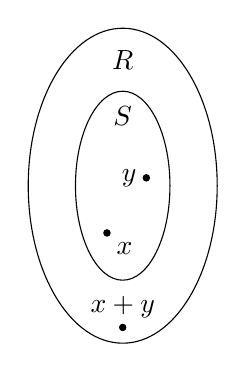
\begin{tikzpicture}[scale=0.4]
  \draw (0,0) ellipse (3 and 5);
  \node at (0,4) {\(R\)};
  \draw (0,0) ellipse (1.5 and 3);
  \draw [fill] (-0.5,-1.5) circle (0.1) node [below right] {\(x\)};
  \draw [fill] (0.75,0.25) circle (0.1) node [left] {\(y\)};
  \draw [fill] (0,-4.5) circle (0.1) node [above] {\(x+y\)};
  \node at (0,2.2) {\(S\)};
\end{tikzpicture}
\caption{Arithmetic in a subset \label{fig:arithmetic-in-a-subset}}
\end{center}
\end{figure}
This is a problem!
The plus and times on a ring must be \emph{closed}.
To avoid this, we single out exactly those subsets of \(R\) for which this does not happen.
That is, the subsets which are closed under the arithmetic on \(R\).

\begin{dfn}[Subring] \label{dfn:subring}
Let \(R\) be a ring and \(S \subseteq R\) a subset. We say that \(S\) is a \DefTerm{subring} of \(R\) if \(S\) is closed under the operations in \(R\). Specifically,
\begin{proplist*}
\item \(0_R \in S\), \label{dfn:subring:zero}
\item If \(x,y \in S\) then \(x+y \in S\), \label{dfn:subring:plus}
\item If \(x \in S\) then \(-x \in S\), and \label{dfn:subring:neg}
\item If \(x,y \in S\) then \(xy \in S\). \label{dfn:subring:times}
\end{proplist*}
If \(R\) is unital, we say that a subring \(S\) is \emph{unital} if in addition \(1_R \in S\). \index{unital!subring}
\end{dfn}

Of course we then have that

\begin{prop} \label{prop:subring-is-ring}
If \(R\) is a ring and \(S \subseteq R\) a subring, then \(S\) is itself a ring under the restricted operations on \(R\). If \(S\) is a unital subring of \(R\), then \(S\) is a unital ring.
\end{prop}

Using the definition, showing that a given sub\emph{set} of a ring is a sub\emph{ring} requires verifying four properties (or five if we want a unital subring). We have a slightly more efficient way to achieve this called the Subring Criterion.

\begin{prop}[Subring Criterion] \label{prop:subring-criterion}
Let \(S \subseteq R\) be a subset. Then \(S\) is a subring of \(R\) if and only if \(S\) is not empty and is closed under subtraction and multiplication. That is, \(S\) is a subring of \(R\) iff the following hold.
\begin{proplist*}
\item \(S \neq \varnothing\).
\item If \(x,y \in S\) then \(x-y \in S\).
\item If \(x,y \in S\) then \(xy \in S\).
\end{proplist*}
\end{prop}

\begin{proof}
First suppose \(S \subseteq R\) is a subring. Then \(S \neq \varnothing\), since \(0_R \in S\). Now if \(x,y \in S\), we have \(xy \in S\), and \(-y \in S\), and \(x + (-y) \in S\). So \(S\) satisfies the Subring Criterion. Conversely, suppose \(S\) satisfies the Subring Criterion. Since \(S\) is not empty, it contains an element \(s\), and since \(S\) is closed under subtraction we have \(0_R = s - s \in S\). Now if \(x\) is any element of \(S\) we have \(-x = 0_R - x \in S\), so that \(S\) is closed under negation. If \(x,y \in S\), then \(x+y = x-(-y) \in S\) and \(xy \in S\). Thus \(S\) is a subring of \(R\).
\end{proof}

The Subring Criterion is a slick way to show that a given subset of a ring is a subring. We have a yet more efficient way to characterize \emph{unital} subrings.

\begin{prop}[Unital Subring Criterion] \label{prop:unital-subring-criterion}
Let \(R\) be a unital ring. Then \(S \subseteq R\) is a unital subring if and only if \(1_R \in S\) and for all \(x,y,z \in S\), \(x-yz \in S\).
\end{prop}

\begin{proof}
Certainly if \(S\) is a unital subring of \(R\) then it satisfies the Unital Subring Criterion. Conversely, suppose \(S\) satisfies the Unital Subring Criterion. Now \(S\) is not empty since \(1_R \in S\). If \(x,y \in S\), then \(x-y = x - 1_R \cdot y \in S\), so that \(S\) is closed under subtraction. Now \(0_R = 1-R - 1_R1_R \in S\) and \(-x = 0_R - 1_R \cdot x \in S\) whenever \(x \in S\), so if \(x,y \in S\) we have \(xy = 0_R - (-x)y \in S\). By the Subring Criterion \(S\) is a subring of \(R\), and since \(1_R \in S\), it is a \emph{unital} subring of \(R\).
\end{proof}

\begin{examples}
\item \textbf{The zero subring.} Let \(R\) be any ring. The subset \(0 = \{0_R\} \subseteq R\) is a subring, called the \emph{zero subring}. (Show it!!)

\item Let \(R\) be a ring and \(k\) a positive integer, and define \(kR = \{ kr \mid r \in R \}\). Then \(kR \subseteq R\) is a subring, but is \emph{not} a unital subring. (@@@)

\item Let \(R\) be any ring and \(a \in R\). Then \(aR = \{ ar \mid r \in R \}\) is a subring of \(R\). (This is the content of \eref{exerc:aR-is-ring}.) Similarly, \(Ra = \{ ra \mid r \in R \}\) is a subring of \(R\). These subrings do not have to be the same!

\item If \(S_1, S_2 \subseteq R\) are (unital) subrings of \(R\), then \(S_1 \cap S_2 \subseteq R\) is also a (unital) subring of \(R\).
\end{examples}

There are two special subrings associated to every ring homomorphism: the \emph{image} and the \emph{kernel}.

\begin{prop}[Image and Kernel] \label{dfn:im-ker}
Let \(\varphi : R \rightarrow S\) be a ring homomorphism. Then we have the following.
\begin{proplist}
\item The set \[ \KER{\varphi} = \{ r \in R \mid \varphi(r) = 0 \}, \] called the \DefTerm{kernel} of \(\varphi\), is a subring of \(R\).
\item The set \[ \IM{\varphi} = \{ s \in S \mid s = \varphi(r)\ \mathrm{for\ some}\ r \in R \}, \] called the \DefTerm{image} of \(\varphi\), is a subring of \(S\).
\end{proplist}
\end{prop}

\begin{proof}
(@@@)
\end{proof}

The image of a homomorphism is everything in the codomain that ``gets hit'', while the kernel is everything in the domain that is ``sent to zero''. We can visualize these subsets as in \autoref{fig:im-ker}.

\begin{figure}[h!]
\begin{center}
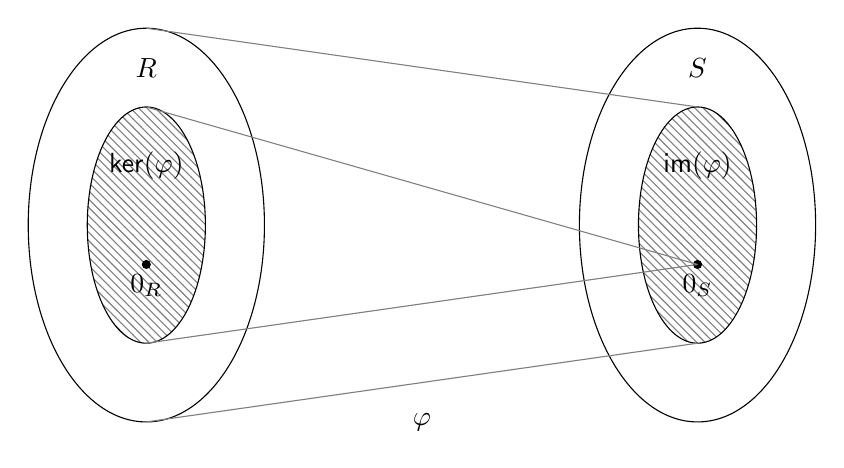
\begin{tikzpicture}[scale=0.5]
  \draw (-7,0) ellipse (3 and 5);
  \node at (-7,4) {\(R\)};
  \draw [pattern=north west lines, pattern color=gray] (-7,0) ellipse (1.5 and 3);
  \draw [fill] (-7,-1) circle (0.1) node [below] {\(0_R\)};
  \node at (-7,1.5) {\(\KER{\varphi}\)};

  \draw (7,0) ellipse (3 and 5);
  \node at (7,4) {\(S\)};
  \draw [pattern=north west lines, pattern color=gray] (7,0) ellipse (1.5 and 3);
  \draw [fill] (7,-1) circle (0.1) node [below] {\(0_S\)};
  \node at (7,1.5) {\(\IM{\varphi}\)};

  \draw [gray] (-7,3) -- (7,-1);
  \draw [gray] (-7,-3) -- (7,-1);
  \draw [gray] (-7,5) -- (7,3);
  \draw [gray] (-7,-5) -- (7,-3);

  \node at (0,-5) {\(\varphi\)};
\end{tikzpicture}
\caption{The image and kernel of a homomorphism. \label{fig:im-ker}}
\end{center}
\end{figure}

The kernels of ring homomorphisms turn out to be very important, as we will see later in \autoref{chap:quot}. As a preview, we can think of homomorphisms \(\varphi : R \rightarrow S\) as projecting a ``shadow'' of \(R\) into \(S\) such that parts of \(R\) get collapsed down in the shadow. The kernel is the part of \(R\) which is collapsed to zero. As a consequence, the kernel measures how badly a homomorphism fails to be injective. Specifically:

\begin{prop} \label{prop:ker-zero}
A ring homomorphism \(\varphi\) is injective if and only if \(\KER{\varphi} = 0\).
\end{prop}

\begin{proof}
Suppose \(\varphi : R \rightarrow S\) is an injective homomorphism. If \(x \in \KER{\varphi}\), then (by definition) we have \(\varphi(x) = 0_S = \varphi(0_R)\). Since \(\varphi\) is injective, we have \(x = 0\). Thus \(\KER{\varphi} = 0\). Conversely, suppose \(\KER{\varphi} = 0\). Now suppose we have \(x,y \in R\) such that \(\varphi(x) = \varphi(y)\). Then \(\varphi(x - y) = \varphi(x) - \varphi(y) = 0\), so that \(x-y \in \KER{\varphi} = 0\). So \(x-y = 0\), and thus \(x = y\). Hence \(\varphi\) is injective.
\end{proof}

We have yet another way to characterize subrings: they are precisely the images of injective ring homomorphisms.

\begin{prop}
Let \(R\) be a ring and \(S \subseteq R\) a subset. The following are equivalent.
\begin{proplist}
\item \(S\) is a subring of \(R\).
\item There is an injective ring homomorphism \(\varphi : T \rightarrow R\) such that \(\IM{\varphi} = S\).
\end{proplist}
\end{prop}

Note that if \(\varphi : R \rightarrow S\) is an injective ring homomorphism, then we have \(R \cong \IM{\varphi}\). This allows us to think of \(R\) as a ``subring'' of \(S\), even though it isn't really, by identifying \(r \in R\) with \(\varphi(r) \in S\). At first this may seem like a trivial observation; we can think of \(R\) as sitting inside \(S\), okay. But suppose \(R\) is a particularly nasty or inconvenient ring to compute in, while \(S\) is very nice -- say, a ring of matrices or numbers. Then \(\varphi\) gives us a way to think of \(R\) in much more convenient terms. An injective mapping \(\varphi : R \rightarrow S\) is sometimes called a \emph{representation} of \(R\), as it literally allows us to ``represent'' elements of \(R\) by elements of \(S\).
\begin{titlebox}{The Representation Problem}
\begin{center}
What are all the representations \(\varphi : R \rightarrow S\) \\ of a ring \(R\) by rings \(S\) having property \(P\)?
\end{center}
\end{titlebox}
Property \(P\) here might be ``is a ring of sets'' or ``is a direct sum of rings of matrices''; typically, any property of rings which makes them particularly nice to compute in.



%---------%
\Exercises%
%---------%

\begin{exercise}
Let \(R = \ZZ\) and \(S \subseteq R\) the set of all prime integers. Show that \(S\) is \emph{not} a subring of \(R\).
\end{exercise}

\begin{exercise}
Let \(a, b > 1\) be relatively prime integers. Show that \(\ZZ/(a) \oplus \ZZ/(b) \cong \ZZ/(ab)\). (Hint: Use \eref{exerc:homs-from-zzn} and \ref{prop:ker-zero})
\end{exercise}

\begin{exercise}
Show that every subring of \(\ZZ\) is of the form \(k\ZZ\) for some \(k\). (@@@) is this true?
\end{exercise}

\begin{exercise}
Let \(R\) be a ring, and let \(e \in R\) be idempotent (that is, \(e^2 = e\)).
\begin{proplist*}
\item Show that \(eRe = \{ ere \mid r \in R \}\) is a subring of \(R\).
\item Show that as a ring, \(S = eRe\) is unital with \(1_S = e\).
\end{proplist*}
In particular, if \(R\) is a unital ring and \(e \neq 1_R\), then \(S\) is not a \emph{unital subring}, even though it is a \emph{subring which is unital}, since in a unital subring \(S\) we have \(1_S = 1_R\).
\end{exercise}

\begin{exercise}
Let \(R\) be a ring, and let \(\mathcal{S}\) be an arbitrary family of subrings of \(R\). Show that \(\bigcap_{S \in \mathcal{S}} S\) is a subring of \(R\).
\end{exercise}

\begin{dfn}[Triangular Matrix, Diagonal Matrix] \label{dfn:triangular-diagonal-matrix}
Let \(R\) be a ring. The set of \(2 \times 2\) \emph{upper triangular} matrices over \(R\) is defined to be \[ \UTMAT{2}{R} = \left\{ \begin{bmatrix} a_{11} & a_{12} \\ 0 & a_{22} \end{bmatrix} \mid a_{11}, a_{12}, a_{22} \in R \right\}. \] Similarly, the set of \(2 \times 2\) \emph{lower triangular} matrices is defined to be \[ \LTMAT{2}{R} = \left\{ \begin{bmatrix} a_{11} & 0 \\ a_{21} & a_{22} \end{bmatrix} \mid a_{11}, a_{12}, a_{22} \in R \right\}, \] and the set of \(2 \times 2\) \emph{diagonal} matrices is defined to be \(\DIAGMAT{2}{R} = \UTMAT{2}{R} \cap \LTMAT{2}{R}\).
\end{dfn}

\begin{exercise}
Let \(R\) be a ring. Show that \(\UTMAT{2}{R}\) and \(\LTMAT{2}{R}\) are subrings of \(\MAT{2}{R}\). Show also that if \(R\) is unital, then \(\UTMAT{2}{R}\) and \(\LTMAT{2}{R}\) are unital subrings.
\end{exercise}

\begin{exercise}
Find the cayley tables of the ring \(\UTMAT{2}{\ZZ/(2)}\).
\end{exercise}

\begin{dfn}[Center] \label{dfn:center}
Let \(R\) be a ring. We define a subset \(\CENTER{R} \subseteq R\) called the \emph{center} as follows. \[ \CENTER{R} = \{ a \in R \mid ax = xa\ \mathrm{for\ all}\ x \in R \} \] That is, the center is the set of all ring elements which commute with every other element of \(R\). For example, \(0_R \in \CENTER{R}\), since if \(x \in R\) we have \(0 \cdot x = 0 = x \cdot 0\). \index{center}
\end{dfn}

\begin{exercise}
Let \(R\) be a ring. Show that the center \(\CENTER{R}\) is a subring of \(R\). Show also that if \(R\) is unital, then \(\CENTER{R}\) is a unital subring of \(R\).
\end{exercise}

\begin{exercise}
Let \(R\) be a unital ring. Show that \[ \CENTER{\MAT{2}{R}} = \left\{ \begin{bmatrix} a & 0 \\ 0 & a \end{bmatrix} \mid a \in \CENTER{R} \right\}. \] (Hint: consider products of \[ \begin{bmatrix} r & 0 \\ 0 & 0 \end{bmatrix} \quad \mathrm{and} \quad \begin{bmatrix} 0 & 1 \\ 0 & 0 \end{bmatrix} \] by an arbitrary element in the center.)
\end{exercise}

\begin{exercise}
Let \(R\) and \(S\) be rings. Show that \(\CENTER{R \oplus S} = \CENTER{R} \oplus \CENTER{S}\).
\end{exercise}

\begin{exercise}
Let \(R\) be a ring and \(A\) a nonempty set. Show that \(\CENTER{R^A} = \CENTER{R}^A\).
\end{exercise}

\begin{dfn}[Nilradical] \label{dfn:nilradical}
If \(R\) is a ring, then the set \(\NILRADICAL{R} \subseteq R\) consisting of all nilpotent elements is called the \emph{nilradical} of \(R\). \index{nilradical}
\end{dfn}

\begin{exercise}
Show that the nilradical of a commutative ring is a subring.
\end{exercise}

\begin{exercise}
Exhibit two matrices \(A, B \in \MAT{2}{\ZZ/(2)}\) such that \(A\) and \(B\) are both nilpotent but \(A + B\) is not nilpotent. (Thus illustrating that commutativity is necessary for the nilradical to be a subring.)
\end{exercise}

\begin{exercise}
Compute the nilradical of the following rings.
\begin{proplist*}
\item \(\ZZ/(5)\)
\item \(\ZZ/(8)\)
\item \(\ZZ/(12)\)
\item \(\ZZ/(30)\)
\end{proplist*}
\end{exercise}

\begin{exercise}[Internal Direct Sums.]
Let \(R\) be a ring, and suppose \(A,B \subseteq R\) are subrings such that \(A + B = R\) and \(A \cap B = 0\).
\begin{proplist}
\item Show that every element of \(A + B\) can be written as \(a + b\) for some \emph{unique} \(a \in A\) and \(b \in B\).
\item Show that \(R \cong A \oplus B\). (In this case we say that \(R\) is an \emph{internal} direct sum of \(A\) and \(B\).)
\end{proplist}
\end{exercise}

\begin{exercise}
If \(R\) is commutative and \(\varphi : R \rightarrow S\) a homomorphism, then the subring \(\IM{\varphi} \subseteq S\) is commutative.
\end{exercise}

\begin{exercise}
Let \(R\) be a ring. Definition \ref{dfn:subring} gives four conditions which a sub\emph{set} \(S \subseteq R\) must satisfy in order to be a sub\emph{ring}. In this exercise we will show that, in general, none of these conditions is redundant. A given subset either does or does not satisfy each condition, giving 16 possibilities. For instance, a given subset may satisfy \sref{dfn:subring}{zero} and \sref{dfn:subring}{plus}, but not \sref{dfn:subring}{neg} or \sref{dfn:subring}{times}.
\begin{proplist}
\item For each of the 12 possible combinations of properties in Definition \ref{dfn:subring} in which either \sref{dfn:subring}{plus} or \sref{dfn:subring}{neg} is \text{not} satisfied, find a subset \(S \subseteq \ZZ\) which satisfies exactly those properties.
\item Show that \(\varnothing \subseteq R\) satisfies \sref{dfn:subring}{plus}, \sref{dfn:subring}{neg}, and \sref{dfn:subring}{times}, but not \sref{dfn:subring}{zero}.
\item Show that \(\{ k\sqrt{2} \mid k \in \ZZ \} \subseteq \ZZ[\sqrt{2}]\) satisfies \sref{dfn:subring}{zero}, \sref{dfn:subring}{plus}, and \sref{dfn:subring}{neg}, but \emph{not} \sref{dfn:subring}{times}.
\item Show that no subset \(S \subseteq R\) can satisfy \sref{dfn:subring}{plus} and \sref{dfn:subring}{neg} but not \sref{dfn:subring}{zero} and \sref{dfn:subring}{times}.
\end{proplist}
\end{exercise}

\begin{dfn}[Exact Sequence]
A \emph{sequence} is a list of ring homomorphisms
\begin{center}
\begin{tikzcd}
R_1 \arrow[r,"\varphi_1"] & R_2 \arrow[r, "\varphi_2"] & \cdots \arrow[r, "\varphi_{n-1}"] & R_n
\end{tikzcd}
\end{center}
We say that a sequence is \emph{exact} \index{exact sequence} if \(\IM{\varphi_i} = \KER{\varphi_{i+1}}\) for each \(i\). As a special case, if the sequence
\begin{center}
\begin{tikzcd}
0 \arrow[r] & A \arrow[r, "\varphi"] & B \arrow[r, "\psi"] & C \arrow[r] & 0
\end{tikzcd}
\end{center}
is exact, we say that the pair \((\varphi, \psi)\) is a \index{short exact sequence} \emph{short exact sequence}.
\end{dfn}

\begin{exercise}
Let \(\varphi : R \rightarrow S\) be a ring homomorphism.
\begin{proplist*}
\item Show that \(0 \rightarrow R \overset{\varphi}{\rightarrow} S\) is exact if and only if \(\varphi\) is injective.
\item Show that \(R \overset{\varphi}{\rightarrow} S \rightarrow 0\) is exact if and only if \(\varphi\) is surjective.
\end{proplist*}
\end{exercise}

\begin{exercise}
Let \(k \in \ZZ\). Show that the following sequence is short exact.
\begin{center}
\begin{tikzcd}
0 \arrow[r] & k\ZZ \arrow[r, "\iota"] & \ZZ \arrow[r, "\pi"] & \ZZ/(k) \arrow[r] & 0
\end{tikzcd}
\end{center}
\end{exercise}

\begin{exercise}
Let \(R\) and \(S\) be rings. Show that the following sequence is short exact.
\begin{center}
\begin{tikzcd}
0 \arrow[r] & R \arrow[r, "\iota_1"] & R \oplus S \arrow[r, "\pi_2"] & S \arrow[r] & 0
\end{tikzcd}
\end{center}
\end{exercise}

\begin{exercise}[Every ring is contained in a unital ring.] \label{exerc:adj-unit}
Let \(R\) be a ring. We define a plus and times on the set \(\ADJUNIT{R} = \ZZ \times R\) by
\begin{eqnarray*}
(a,r) + (b,s) & = & (a+b,r+s) \\
(a,r) \cdot (b,s) & = & (ab, as + br + rs)
\end{eqnarray*}
Show the following.
\begin{proplist}
\item These operations make \(\ADJUNIT{R}\) a unital ring.
\item The map \(\iota : R \rightarrow \ADJUNIT{R}\) given by \(\iota(r) = (0,r)\) is an injective ring homomorphism.
\item If \(S\) is a unital ring and \(\varphi : R \rightarrow S\) a ring homomorphism, then there is a unique unital ring homomorphism \(\Theta : \ADJUNIT{R} \rightarrow S\) such that the following diagram commutes.
\begin{center}
\begin{tikzcd}
R \arrow[d,"\iota"'] \arrow[rd,"\varphi"] & \\
\ADJUNIT{R} \arrow[r,"\Theta"'] & S
\end{tikzcd}
\end{center}
\end{proplist}
\end{exercise}

\begin{exercise}[A representation theorem for unital rings.]
Let \(R\) be a ring, and let \(R^0\) be the nullification of \(R\) (cf. (@@@)). Denote by \(\ast\) the null product on \(R^0\); that is, \(r \ast s = 0\) for all \(r,s \in R\). Recall (cf. (@@@)) that \(\END{R^0}\) is a ring under pointwise addition and function composition.
\begin{proplist}
\item Given \(r \in R\), define \(\mu_r : R^0 \rightarrow R^0\) by \(\mu_r(a) = ra\). Show that \(\mu_r\) is a ring homomorphism.
\item Show that \(\Psi : R \rightarrow \END{R^0}\) given by \(\Psi(r) = \mu_r\) is a ring homomorphism.
\item Show that if \(R\) is unital then \(\Psi\) is injective.
\end{proplist}
That is, every unital ring is isomorphic to a ring of endomorphisms of a null ring. Combined with \eref{exerc:adj-unit}, \emph{every} ring is isomorphic to a ring of endomorphisms of a null ring.
\end{exercise}

(Extended example - Generated Subrings?)

      \newpage

    \section{Domains and Fields}
      \label{sec:domains-and-fields}
      In College Algebra, how might we go about solving an equation like \(2x = 6\) in the rational numbers? There are essentially two different, but related, strategies.

The simplest idea is to multiply both sides of the equation by \(1/2\).
Why \(1/2\)? Because that is precisely the number which, when multiplied by \(2\), yields \(1\), the multiplicative identity.
The numbers \(2\) and \(1/2\) enjoy this relationship with one another, just like \(3\) and \(1/3\) or \(5/7\) and \(7/5\).
But if \(r\) is an arbitrary element of an arbitrary ring \(R\), there may be no way to find a special element like \(\frac{1}{r}\) with the property that \(r \cdot \frac{1}{r} = 1_R\).
Such elements are very precious, so they get a name.

\begin{dfn}[Unit] \label{dfn:unit-field}
Let \(R\) be a unital ring.
\begin{proplist}
\item We say that \(u \in R\) is a \emph{unit}\index{unit} if there is an element \(u^{-1} \in R\), called an \emph{inverse} of \(u\), such that \(uu^{-1} = u^{-1}u = 1_R\).
\item We say that \(R\) is a \emph{field}\index{field} if \(R\) is commutative and every nonzero element of \(R\) is a unit.
\end{proplist}
\end{dfn}

\begin{examples}
\item In any unital ring, \(1_R\) is a unit.

\item In \(\ZZ\) the only units are \(1\) and \(-1\).
\end{examples}

\begin{prop} \label{prop:unit-basics}
Let \(R\) be a unital ring.
\begin{proplist}
\item \label{prop:unit-basics:unique} If \(u \in R\) is invertible, then \(u^{-1}\) is unique in the following sense: if \(v \in R\) such that \(uv = vu = 1_R\), then \(v = u^{-1}\).
\item If \(\varphi : R \rightarrow S\) is a unital homomorphism and \(u \in R\) is a unit, then \(\varphi(u)\) is a unit and \(\varphi(u)^{-1} = \varphi(u^{-1})\).
\end{proplist}
\end{prop}

\begin{proof}
\begin{inlineproplist}
\item Note that \(v = v \cdot 1_R = v \cdot u \cdot u^{-1} = 1 \cdot u^{1} = u^{-1}\).
\item Note that \(1_S = \varphi(1_R) = \varphi(uu^{-1}) = \varphi(u)\varphi(u^{-1})\), and similarly \(1_S = \varphi(u^{-1})\varphi(u)\).
Thus \(\varphi(u)\) is invertible, and we have \(\varphi(u^{-1}) = \varphi(u)^{-1}\) by \paref{prop:unit-basics:unique}.
\end{inlineproplist}
\end{proof}

Let's revisit our motivating equation \(2x = 6\).
Another way to solve this equation is to rewrite it as \(2x - 6 = 0\), and then factor as \(2(x-3) = 0\).
Now the integers have the following very nice ``zero product property'':
\begin{center}
If \(a\) and \(b\) are integers and \(ab = 0\), then either \(a = 0\) or \(b = 0\).
\end{center}
From here we can break our equation into two: either \(2 = 0\) or \(x - 3 = 0\).
Of course the first case is absurd (in \(\ZZ\)!) so we conclude that \(x - 3 = 0\), so \(x = 3\).
The zero product property is also what allows the factorization method of solving equations.
For instance, to solve an equation like \(x^2 - 5x - 6 = 0\) over the integers, we factor the left hand side as \((x-2)(x-3) = 0\).
Using the zero product property, either \(x-2 = 0\) (so \(x = 2\)) or \(x-3 = 0\) (so \(x = 3\)).

A given ring may or may not have this property.
While \(\ZZ\) does, \(\ZZ/(n)\), for instance, may not; in \(\ZZ/(6)\) we have \(2 \neq 0\) and \(3 \neq 0\), but \(2 \cdot 3 = 0\).
In this case we say that \(2\) and \(3\) are zerodivisors in \(\ZZ/(6)\).

\begin{dfn}[Zerodivisor] \label{dfn:zerodivisor-domain}
Let \(R\) be a commutative ring.
\begin{proplist}
\item We say that a nonzero element \(r \in R\) is a \emph{zerodivisor}\index{zerodivisor} if there is a nonzero element \(s \in R\) such that \(rs = 0\).
\item We say that a commutative unital ring \(R\) is an \emph{integral domain}\index{domain}, or simply \emph{domain}, if \(R\) does not contain any zero divisors.
\end{proplist}
\end{dfn}

Note that this definition of zerodivisor applies only to \emph{commutative} rings.
Generalization to noncommutative rings is left to the exercises.

\begin{prop}[Cancellation] \label{prop:cancellation}
Let \(R\) be a domain with \(r,s,t \in R\).
If \(rs = rt\) and \(r \neq 0\), then \(s = t\).
\end{prop}

\begin{proof}
If \(rs = rt\), then \(rs - rt = 0\), so that \(r(s-t) = 0\).
Since \(r \neq 0\), we must have \(s-t = 0\), so that \(s = t\).
\end{proof}


\begin{prop}
Every field is also an integral domain.
\end{prop}

\begin{proof}
Let \(R\) be a field; in particular \(R\) is commutative.
We need to show that \(R\) does not contain any zero divisors.
To this end, suppose \(r,s \in R\) such that \(rs = 0\).
If \(r \neq 0_R\), then \(r\) is a unit in \(R\).
Now \(r^{-1}rs = 0_R\), so that \(1_R \cdot s = 0_R\), and thus \(s = 0_R\).
That is, either \(r = 0_R\) or \(s = 0_R\).
So \(R\) does not contain any zero divisors.
\end{proof}



%---------%
\Exercises%
%---------%

\begin{exercise}
Show that if \(R\) and \(S\) are nontrivial rings, then \(R \oplus S\) is \emph{not} a domain.
\end{exercise}

\begin{exercise}
Show that every subring of a domain is a domain.
In particular, every subring of a field is a domain.
\end{exercise}

\begin{exercise}
Show that every domain (hence every field) has characteristic 0 or a prime.
(cf. \ref{dfn:characteristic})
\end{exercise}

\begin{exercise}
Find an example of two unital rings \(R\) and \(S\), a ring homomorphism \(\varphi : R \rightarrow S\), and a unit \(u \in R\) such that \(\varphi(u) \in S\) is \emph{not} a unit.
(Hint: By (@@@) \(\varphi\) cannot be unital.)
\end{exercise}

\begin{exercise}
Show that \(\ZZ/(n)\) is a field if and only if \(n\) is prime.
\end{exercise}

\begin{dfn}[Group of Units]
Let \(R\) be a unital ring.
The \emph{group of units} of \(R\) is the set \(\UNITS{R} = \{ u \in R \mid u\ \mathrm{is\ a\ unit} \}\).
\end{dfn}

\begin{exercise} \label{exerc:units-form-group}
Let \(R\) be a unital ring.
Show that the following hold.
\begin{proplist*}
\item \(1_R\) is a unit.
\item If \(u, v \in \UNITS{R}\), then \(uv \in \UNITS{R}\).
\item If \(u \in \UNITS{R}\), then \(u^{-1} \in \UNITS{R}\).
\end{proplist*}
\end{exercise}

\begin{exercise}
Show that \(\UNITS{\ZZ} = \{ 1, -1 \}\).
\end{exercise}

\begin{exercise}
Show that \(\UNITS{\ZZ/(n)} = \{ [a] \in \ZZ/(n) \mid \GCD{a}{n} = 1 \}\).
\end{exercise}

\begin{exercise}
Let \(X\) be a nonempty set.
Show that \(\UNITS{\POW{X}} = \{X\}\).
\end{exercise}

\begin{exercise}
Let \(A\) be a CU ring.
Show that \[ \UNITS{\MAT{2}{A}} = \left\{ \begin{bmatrix} a & b \\ c & d \end{bmatrix} \mid ad - bc\ \mathrm{is\ a\ unit\ in}\ A \right\}. \]
\end{exercise}

\begin{exercise}
Show that if \(R\) is a domain, then the nilradical of \(R\) is \(0\).
(cf. \autoref{dfn:nilradical})
\end{exercise}

\begin{exercise}[Every finite domain is a field.]
Let \(R\) be a \emph{finite} integral domain.
In this exercise we will show that \(R\) must be a field.
\begin{proplist}
\item Let \(r \in R\) be a nonzero element and define a mapping \(\varphi_r : R \rightarrow R\) by \(\varphi_r(x) = rx\).
Show that \(\varphi_r\) must be injective.
\item Deduce that \(\varphi_r\) must be bijective.
\item Deduce that \(r\) must be a unit in \(R\), and then that \(R\) must be a field.
\end{proplist}
\end{exercise}

\begin{dfn}[Fractional Integers] \label{dfn:fractional-integers}
Let \(k \in \ZZ\) with \(k \neq 0\).
We define the set of \emph{fractional integers} with denominator \(k\) to be \[ \ZZFRAC{k} = \left\{ \frac{a}{k^t} \mid a \in \ZZ, t \in \NN \right\} \subseteq \QQ. \]
\end{dfn}

\begin{exercise}
Show that \(\ZZFRAC{k}\) is a unital subring of \(\QQ\).
\end{exercise}

\begin{exercise}
Show that the units in \(\ZZFRAC{k}\) are of the form \(\frac{\pm 1}{2^t}\) or \(\pm 2^t\) where \(t \in \NN\).
\end{exercise}

\begin{exercise}
Give an example of a (nonunital) ring homomorphism \(\varphi : R \rightarrow S\) and an element \(u \in R\) such that \(u\) is a unit in \(R\) but \(\varphi(u)\) is not a unit in \(S\).
\end{exercise}

(@@@) one-sided zerodivisors and units

(@@@) zero divisor graph

\textbf{Skew fields.}

      \newpage

    \section{Quadratic Extensions}
      \label{sec:quad-ext}
      In this section we will pause to construct an important family of example rings.

\begin{dfn}[Quadratic Extension]
Let \(R\) be a commutative ring, and let \(D \in R\).
We define the \emph{quadratic extension}\index{quadratic extension} of \(R\) by \(D\) to be \(R[\sqrt{D}] = R \times R\) as a set, and define operations on \(R[\sqrt{D}]\) as follows.
\begin{eqnarray*}
(r_1,r_2) + (s_1,s_2) & = & (r_1+s_1, r_2+s_2) \\
(r_1,r_2) \cdot (s_1,s_2) & = & (r_1s_1 + Dr_2s_2, r_1s_2 + r_2s_1)
\end{eqnarray*}
We will write the element \((a,b) \in R[\sqrt{D}]\) as \(a + b\sqrt{D}\).
\end{dfn}

The notation \(R[\sqrt{D}]\) is intended to suggest that this structure behaves much like \(R\), but now the element \(D\) has a ``square root''.
It's important to remember that the plus in \(a + b\sqrt{D}\) is a \emph{structural} symbol, not an operation symbol.

\begin{prop} \label{prop:quad-ext-ring}
Let \(R\) be a ring and \(D \in R\).
\begin{proplist*}
\item \(R[\sqrt{D}]\) is a commutative ring.
\item If \(R\) is unital, then \(R[\sqrt{D}]\) is unital.
\item The map \(\iota : R \rightarrow R[\sqrt{D}]\) given by \(\iota(r) = (r,0_R)\) is a ring homomorphism.
If \(R\) is unital, then \(\iota\) is unital.
\end{proplist*}
\end{prop}

The most important use of quadratic extensions is to construct new domains and fields out of old ones.

\begin{prop} \label{prop:quad-ext-dom} \mbox{}
\begin{proplist}
\item If \(R\) is a domain, then \(R[\sqrt{D}]\) is a domain if and only if the equation \(Dy^2 = x^2\) has no nonzero solutions in \(R\).
\item If \(R\) is a field, then \(R[\sqrt{D}]\) is a field if and only if the equation \(D = x^2\) has no nonzero solutions in \(R\).
\end{proplist}
\end{prop}

\begin{proof}
\begin{inlineproplist}
\item (@@@)
\item (@@@)
\end{inlineproplist}
\end{proof}

\begin{prop} \label{prop:sqfree-int}
Let \(D\) be an integer.
We say that \(D\) not equal to 0 or 1 is \emph{squarefree}\index{squarefree!integer} if \(D\) is not divisible by \(a^2\) for any \(a > 1\).
\begin{proplist}
\item \label{prop:sqfree-int:zz-dom} If \(D\) is squarefree, then the equation \(Dy^2 = x^2\) has no nonzero solutions in \(\ZZ\), and thus \(\ZZ[\sqrt{D}]\) is a domain.
\item \label{prop:sqfree-int:qq-field} If \(D\) is squarefree, then the equation \(D = x^2\) has no solutions in \(\QQ\), and thus \(\QQ[\sqrt{D}]\) is a field.
\end{proplist}
\end{prop}

\begin{proof}
\begin{inlineproplist}
\item We consider two cases: if \(|D| \leq 1\) and if \(|D| > 1\).
In the first case, \(D = -1\).
Now if \(Dy^2 = x^2\), then we have \(-y^2 = x^2\); by sign considerations we have \(x = y = 0\).
In the second case, \(D\) is divisible by a prime, say \(p\).
If \(x = 0\), then \(y = 0\), and likewise if \(y = 0\) then \(x = 0\), so we can assume \(x\) and \(y\) are both nonzero.
By the fundamental theorem of arithmetic, \(p\) appears the same number of times in the factorizations of \(Dy^2\) and \(x^2\).
But note that \(p\) must appear an even number of times in \(x^2\), but an odd number of times in \(Dy^2\), a contradiction.
Thus in either case the equation \(Dy^2 = x^2\) has no nonzero solutions.
\item If \(D = x^2\) has a rational solution \(x = p/q\), then \(Dq^2 = p^2\), which contradicts \ref{prop:sqfree-int:zz-dom}.
\end{inlineproplist}
\end{proof}

There are plenty of squarefree integers; in fact these are precisely the integers with no repeated prime factors.
Each such integer yields a different domain \(\ZZ[\sqrt{D}]\) and field \(\QQ[\sqrt{D}]\).
These rings are particularly nice for a few reasons.
They are easy to compute in, and while similar to \(\ZZ\) and \(\QQ\), can exhibit wildly different behavior, as we will see in the next chapter.




%---------%
\Exercises%
%---------%

\begin{exercise}
Prove Proposition \ref{prop:quad-ext-ring}.
\end{exercise}

\begin{exercise}
Let \(R = \ZZ/(3)\).
\begin{proplist}
\item Show that \(2x^2 = y^2\) has no nonzero solutions in \(R\).
(Hint: When in doubt, use brute force.)
\item Conclude that \(R[\sqrt{2}]\) is a field with 9 elements.
\end{proplist}
\end{exercise}

\begin{exercise}
Elements of \(\ZZ[\sqrt{-1}]\) are sometimes called \emph{gaussian integers}.
\begin{proplist}
\item Determine which elements of \(\ZZ[\sqrt{-1}]\) are units.
\end{proplist}
\end{exercise}

\begin{exercise}
Show that \(\CHAR{R} = \CHAR{R[\sqrt{D}]}\).
\end{exercise}

\begin{exercise}
Let \(R\) be a ring and \(S \subseteq R\) a subring, with \(D \in S\).
Show that \(S[\sqrt{D}]\) is a subring of \(R[\sqrt{D}]\).
\end{exercise}

\begin{exercise}
Let \(\varphi : R \rightarrow S\) be a ring homomorphism with \(D \in R\) and \(E = \varphi(D)\).
Show that there is a unique ring homomorphism \(\Phi : R[\sqrt{D}] \rightarrow S[\sqrt{E}]\) such that the following diagram commutes.
\begin{center}
\begin{tikzcd}
R \arrow[r,"\varphi"] \arrow[d, "\iota"']    & S \arrow[d, "\iota"] \\
R[\sqrt{D}] \arrow[r, "\Phi"'] & S[\sqrt{E}]
\end{tikzcd}
\end{center}
\end{exercise}

      \newpage

    \section{Divisibility}
      \label{sec:divisibility}
      In addition to the arithmetic structure, the ring of integers has a \emph{divisibility structure} which we are able to use to some effect.
This is the language we use in \(\ZZ\) to say things about greatest common divisors and unique factorization.
And so we carry the ``divides'' concept to any commutative ring.

\begin{dfn}[Divides] \label{dfn:divides}
Let \(R\) be a commutative ring with \(a,b \in R\).
We say \(a\) \emph{divides}\index{divides} \(b\), denoted \(a|b\), if there is an element \(c \in R\) such that \(b = ac\).
In this case we say that \(a\) is a \emph{divisor} of \(b\).
\end{dfn}

Divisibility captures some of the multiplicative structure on \(R\) and, as a relation, enjoys some of the familiar properties from \(\ZZ\).

\begin{prop} \label{prop:divides-basics}
Let \(R\) be a commutative ring with \(a,b,c \in R\).
Then we have the following.
\begin{proplist*}
\item \label{prop:divides-basics:refl} \(a|a\).
\item \label{prop:divides-basics:trans} If \(a|b\) and \(b|c\) then \(a|c\).
\item \label{prop:divides-basics:zero} \(a|0\).
\end{proplist*}
\end{prop}

\begin{proof}
\begin{inlineproplist}
\item We have \(a = a \cdot 1\), so \(a|a\).
\item Suppose \(a|b\) and \(b|c\); then there exist \(h,k \in R\) such that \(b = ah\) and \(c = bk\).
Now \(c = a(hk)\), so that \(a|c\).
\item \(0 = a \cdot 0\) as needed.
\end{inlineproplist}
\end{proof}

If \(R\) is unital, we can say a bit more.

\begin{prop} \label{prop:divides-u-basics}
Let \(R\) be a CU ring and \(a,u \in R\) with \(u\) a unit.
\begin{proplist*}
\item \label{prop:divides-u-basics:one} \(1|a\) for all \(a \in R\).
\item \label{prop:divides-u-basics:unit} If \(u \in R\) is a unit, then \(u|a\).
\item \label{prop:divides-u-basics:unit-div} If \(u \in R\) is a unit and \(a|u\), then \(a\) is a unit.
\end{proplist*}
\end{prop}

\begin{proof}
\begin{inlineproplist}
\item Note that \(a \cdot 1 = a\).
\item First note that \(a = 1 \cdot a\), so that \(1|a\).
Now if \(u \in R\) is a unit, then by definition we have an element \(v\) such that \(1 = uv\), so that \(u|1\).
By \sref{prop:divides-basics}{trans} we have \(u|a\).
\item Say \(ab = u\).
Now \(abu^{-1} = 1_R\), and thus \(a\) is a unit.
\end{inlineproplist}
\end{proof}

We should not let our intuition about divisibility in \(\ZZ\) go too far, though, as divisibility in an arbitrary commutative ring can be very strange.
For example, in \(\ZZ\) if \(a|b\) then in a specific sense \(a\) is ``smaller than'' \(b\), and we cannot have never-ending chains of integers, each divisible by the next.
This alone makes \(\ZZ\) very special.
In fact \autoref{chap:domains} is devoted to understanding how divisibility in \(R\) is different from divisibility in \(\ZZ\), at least when \(R\) is a domain.

Two ring elements which differ only by a unit factor are indistinguishable from the perspective of divisibility; we call such pairs \emph{associates}.

\begin{dfn}[Associate] \label{dfn:associate}
Let \(R\) be a CU ring.
If \(a,b \in R\), we say \(a\) \emph{is associate to}\index{associate} \(b\), denoted \(a \ASSOC b\), if there is a \emph{unit} \(u \in R\) such that \(b = ua\).
\end{dfn}

We will say quite a bit more about associate elements in \autoref{chap:domains}.
For now, to help get a handle on the concept, we consider only two special cases.

\begin{prop}
Let \(R\) be a CU ring.
\begin{proplist*}
\item If \(0_R \ASSOC a\) then \(a = 0_R\).
\item \(1_R \ASSOC a\) if and only if \(a\) is a unit.
\item If \(a \ASSOC b\), then \(ac \ASSOC bc\).
\end{proplist*}
\end{prop}

\begin{proof}
\begin{inlineproplist}
\item There is a unit \(u\) with \(a = u0_R = 0_R\).
\item There is a unit \(u\) with \(a = u1_R = u\).
\item If \(b = ua\) for some unit \(u\); then also \(bc = uac\).
\end{inlineproplist}
\end{proof}

In a CU ring, every element is divisible by (1) units and (2) its associates.
These are called \emph{trivial divisors}.
In general, a ring element will have more divisors.
Some ring elements, however, have \emph{only} the trivial divisors.
These are special.
In \(\ZZ\), such elements are called \emph{prime}.
However, for some very good reasons that will be made clear later, in a general ring such elements are called \emph{irreducible}.

\begin{dfn}[Irreducible] \label{dfn:irreducible-element}
Let \(R\) be a CU ring and \(x \in R\) a nonzero nonunit.
We say that \(x\) is \emph{irreducible}\index{irreducible} in \(R\) if, whenever \(a,b \in R\) such that \(x = ab\), either \(a\) or \(b\) is a unit.
\end{dfn}

For example, in \(\ZZ\) the irreducible elements are precisely the prime integers in the usual sense.
If \(R\) is a field, then by a quirk of logic \(R\) has no irreducible elements.
(There are no nonzero nonunits!)

It is somewhat unfortunate that our most immediate examples of irreducible elements are the prime integers -- you may be wondering why we use the word ``irreducible'' for the generalized concept.
But recall that there are in fact two different ways to characterize the prime integers; these are discussed in \ref{dfn:zz-prime} and \ref{prop:zz-prime-2}.
In \(\ZZ\) these two are equivalent, but in a general ring they are not -- so we split the familiar concept of \emph{primeness} into two.

\begin{dfn}[Prime] \label{dfn:prime-element}
Let \(R\) be a CU ring and \(p \in R\) a nonzero nonunit.
We say that \(p \in R\) is \emph{prime}\index{prime!element} if whenever \(p|ab\), either \(p|a\) or \(p|b\) (or both).
\end{dfn}

The distinction between ``irreducible'' and ``prime'' is a subtle one; at first glance we've simply replaced the equality by divisibility.
Roughly, \emph{irreducible} means \emph{has no nontrivial divisors}, while \emph{prime} means \emph{cannot be nontrivially decomposed}.
These two ideas are equivalent in \(\ZZ\), as we know, but different in general.
They are related, however, as in the following result.

\begin{prop}
If \(R\) is a domain, then every prime element is also irreducible.
\end{prop}

\begin{proof}
Suppose \(p \in R\) is prime, and factor \(p\) as \(p = ab\).
In particular, \(p|ab\), and since \(p\) is prime, WLOG we have \(p|a\).
Say \(a = pt\).
Now \(p = ab = ptb\), and by cancellation, \(tb = 1\).
In particular \(b\) is a unit.
Thus \(p\) is irreducible.
\end{proof}



%---------%
\Exercises%
%---------%

\begin{exercise}
Find all the divisors of 4 in \(\ZZ\).
Prove that your list is complete.
\end{exercise}

\begin{exercise}
Let \(X\) be a nonempty set, and let \(A,B \in \POW{X}\).
Show that \(A|B\) if and only if \(B \subseteq A\).
\end{exercise}

\begin{exercise}
Let \(R\) and \(S\) be rings, with \((a,b), (r,s) \in R \oplus S\).
Show that \((a,b) | (r,s)\) if and only if \(a|r\) and \(b|s\).
\end{exercise}

\begin{exercise}
(@@@) if \(R\) is not a domain, yadda yadda converse of last exercise.
\end{exercise}

\begin{exercise}
Let \(\varphi : R \rightarrow S\) be a ring homomorphism with \(a,b \in R\).
Show that if \(a|b\), then \(\varphi(r)|\varphi(s)\).
\end{exercise}

\begin{exercise}
Let \(R = \POW{\NN}\) and consider the elements of \(R\) of the form \(r_k = [1,k]\).
Show that \(r_k|r_\ell\) if and only if \(k \geq \ell\).
\end{exercise}

\begin{exercise} \label{exerc:assoc-equiv}
Let \(R\) be a CU ring.
Show that ``is associate to'' is an equivalence relation.
\end{exercise}

\begin{exercise} \label{exerc:associate-divides}
Let \(R\) be a CU ring.
Show that the following hold.
\begin{proplist*}
\item \label{exerc:associate-divides:divide-R} If \(x \ASSOC y\), then \(z|x\) if and only if \(z|y\) for all \(z \in R\).
\item \label{exerc:associate-divides:divide-L} If \(x \ASSOC y\), then \(x|z\) if and only if \(y|z\) for all \(z \in R\).
\end{proplist*}
\end{exercise}

\begin{exercise}
Let \(R\) be a domain with \(a,b \in R\).
Show that if \(a|b\) and \(b|a\) then \(a \ASSOC b\).
\end{exercise}

\begin{exercise}
Let \(R\) be a domain with \(a,b,c \in R\).
Show that if \(ac|bc\) then \(a|b\).
\end{exercise}

\begin{exercise}
Let \(R\) be a domain and \(a,b \in R\) such that \(a \ASSOC b\).
Show that the following hold.
\begin{proplist*}
\item If \(a\) is irreducible, then \(b\) is irreducible.
\item If \(a\) is prime, then \(b\) is prime.
\end{proplist*}
\end{exercise}

\begin{exercise}
Let \(R\) be a domain with \(a,b,c \in R\) and \(c \neq 0\).
Show that if \(ac \ASSOC bc\), then \(a \ASSOC b\).
\end{exercise}

\begin{exercise}
Let \(R\) and \(S\) be CU rings.
Show that \((r_1,s_1) \ASSOC (r_2,s_2)\) in \(R \oplus S\) if and only if \(r_1 \ASSOC r_2\) in \(R\) and \(s_1 \ASSOC s_2\) in \(S\).
\end{exercise}

\begin{exercise}
Definition \ref{dfn:divides} requires \(R\) to be a commutative ring, but is this really necessary? (Divisibility in noncommutative rings.)
\end{exercise}

      \newpage

    \section{Norms}
      \label{sec:norms}
      In \(\ZZ\) there are lots of neat things we can do with irreducibles.
Every integer is a product of irreducibles, \(\ZZ/(n)\) is a field precisely when \(n\) is irreducible, and algorithms for detecting irreducibles have practical applications.
In a general ring we might hope that some of these neat things generalize.
First, we need to be able to detect whether or not an element is irreducible.
In \(\ZZ\) we have a brute-force algorithm for this thanks to induction, but most rings do not have an obvious analogue of this strategy.

In some rings (not all!) we can make progress on the problem of finding irreducibles by mapping the multiplicative structure of \(R\) to the \(\NN\) -- doing this we can take advantage of what we know about natural numbers and, sometimes, recover the benefits of induction.

\begin{dfn}[Norm] \label{dfn:norm}
Let \(R\) be a domain.
A mapping \(N : R \rightarrow \NN\) is called a \emph{norm}\index{norm} if the following hold.
\begin{itemize}
\item[N1.] \(N(\alpha) = 0\) iff \(\alpha = 0\).
\item[N2.] If \(\alpha,\beta \in R\) are nonzero then \(N(\alpha) \leq N(\alpha\beta)\).
\end{itemize}
We say \(N\) is \emph{multiplicative} if it satisfies the additional constraint that
\begin{itemize}
\item[N3.] \(N(\alpha\beta) = N(\alpha)N(\beta)\) for all \(\alpha, \beta \in R\).
\end{itemize}
\end{dfn}

\begin{examples}
\item \(N : \ZZ \rightarrow \NN\) given by \(N(a) = |a|\) is a multiplicative norm.
\item \(N : \ZZ[i] \rightarrow \NN\) given by \(N(a+bi) = a^2 + b^2\) is a multiplicative norm.
\item More generally, \(N : \mathcal{O}(\sqrt{D}) \rightarrow \NN\) given by \(N(a+b\sqrt{D}) = |a^2 + Db^2|\) if \(D \equiv 2,3 \mod 4\) and \(N(a+b\frac{1+\sqrt{D}}{2}) = |a^2 + ab + b^2\frac{1-D}{4}|\) if \(D \equiv 1 \mod 4\) is a multiplicative norm.
\item If \(R\) has a norm \(N\), then the quadratic extension of \(R\) by \(D\) has a norm \(M(a + b\sqrt{D}) = N(a^2 - Db^2)\).
(@@@)
\end{examples}

If a ring has a multiplicative norm, we can use it to detect (some) irreducible elements.

\begin{prop}
Let \(R\) be a domain and \(N : R \rightarrow \NN\) a multiplicative norm.
If \(\alpha \in R\) such that \(N(\alpha)\) is prime in \(\NN\), then \(\alpha\) is irreducible in \(R\).
\end{prop}

For example, consider \(\ZZ[i]\).
Applying this result here, we see that \(a \pm bi\) is irreducible if \(a^2 + b^2\) is prime.
In particular \(1 \pm i\), \(1 \pm 2i\), \(2 \pm 3i\), and many other Gaussian integers are irreducible (since \(1^2 + 1^2 = 2\), \(1^2 + 2^2 = 5\), and \(2^2 + 3^2 = 13\) are prime).
This leads to a natural question about the natural numbers: for which primes \(p\) does the equation \(a^2 + b^2 = p\) have a solution?

As this example shows, a good multiplicative norm can turn questions in \(R\) into number theory problems.
This turns out to be a useful technique more generally: given a problem about some object, look for a way to map the relevant structure of that object to some other object which either is well-understood or with which we can compute things.
A good strategy for solving algebraic problems is to try to reduce to number theory or to linear algebra.



%---------%
\Exercises%
%---------%

\begin{exercise}
Let \(F\) be a field.
Show that the map \(N : F \rightarrow \NN\) given by \[ N(x) = \left\{ \begin{array}{ll} 0 & \mathrm{if}\ x = 0_F \\ 1 & \mathrm{otherwise} \end{array} \right. \] is a multiplicative, unit-preserving norm.
\end{exercise}

\begin{exercise}
Let \(D\) be a squarefree integer.
\begin{proplist}
\item Show that (@@@) given by (@@@) is a multiplicative norm.
\item Show that if \(D < -1\), then the units in (@@@) are \(\pm 1\).
\end{proplist}
\end{exercise}

\begin{exercise}
Let \(R\) be a domain and \(N\) a multiplicative norm on \(R\).
\begin{proplist}
\item Show that \(N(1) = 1\).
\item Show that \(N(u) = 1\) for any unit \(u\).
\end{proplist}
\end{exercise}

\begin{exercise}
Draw the Hasse diagram of divisors of \(2\sqrt{-2}\) in zee adjoin sqrt minus 2.
(@@@) make this one multipart
\end{exercise}

\begin{dfn}
We say a norm is \emph{unit-separating} if \(N(x) = 1\) implies that \(x\) is a unit.
\end{dfn}

      \newpage

    \phantomsection
    \section*{Summary of \autoref{chap:rings}}
      \addcontentsline{toc}{section}{Summary}%&%
      \input{src/ring/1.X-summary.tex}


  \chapter{The Domain Hierarchy}
    \label{chap:domains}
    In \autoref{chap:rings} we defined a class of structures, called \emph{rings}, which generalize the basic arithmetic on \(\ZZ\) and \(\ZZ/(n)\). The ring of integers comes equipped with some extra technology which turns out to be useful: specifically, the \textbf{division algorithm}, \textbf{unique factorization}, and the existence of \textbf{greatest common divisors}. In this chapter we will see how this technology generalizes (or not!) to other rings -- to integral domains, in particular. At the risk of giving away the punchline, we will see that the technology on \(\ZZ\), when reimagined in arbitrary domains, gives rise to a \textbf{hierarchy} of families of domains of increasing algorithmic power.

    \newpage

    \section{Associates}
      \label{sec:associates}
      Recall that if \(R\) is a CU ring, we say that two elements \(a,b \in R\) are \emph{associate}, denoted \(a \ASSOC b\), if there is a unit \(u \in R\) such that \(a = ub\).
It turns out that the divisibility structure of \(R\) cannot distinguish associates from each other.
Considering associate elements to be ``the same'', we have a nice way to visualize the divisibility structure of a ring.

Recall that if \(\sigma\) is an equivalence relation on a set \(X\), then we have a canonical \emph{partition} of \(X\) induced by \(\sigma\) given by the \(\sigma\)-classes.
This partition, considered as a set, is called the \emph{quotient} of \(X\) by \(\sigma\), and acts very much like \(X\) does except that elements of \(X\) which are \(\sigma\) related become equal in \(X/\sigma\).
This is a powerful idea which we will use again in \autoref{chap:quot}.
For now, we will use the classes of the associate relation to reason about divisibility.

\begin{dfn}[Associate Structure] \label{dfn:assoc-sld}
Let \(R\) be a CU ring.
Recall by \eref{exerc:assoc-equiv} that \(\ASSOC\) is an equivalence relation on \(R\).
The set \(\ASSOCLAT{R} = R/\!\!\ASSOC\) of all \(\ASSOC\)-equivalence classes of \(R\) is called the \emph{associate structure} of \(R\).
\end{dfn}

Note that, by definition, the associate class of \(a\) is all the elements of the form \(ua\) where \(u\) is a unit.
If \(R\) is small enough we can find its associate classes by hand.
For example, the associate classes of \(\ZZ/(4)\) are \([0] = \{0\}\), \([1] = \{1,3\}\), and \([2] = \{2\}\).
The ring \(\ZZ\) is not very small, but we can see that its associate classes are \([0]\) and \([n] = \{ n, -n \}\) where \(n > 0\).
As promised, the divisibility relation on \(R\) can be bumped up to a kind of relation on \(\ASSOCLAT{R}\).

\begin{prop}
Let \(R\) be a CU ring.
We define a relation \(\lesssim\) on \(\ASSOCLAT{R}\) as follows: given two associate classes \(A\) and \(B\), we say \(A \lesssim B\) if there exist \(a \in A\) and \(b \in B\) such that \(a|b\).
Then the following hold for all \(A,B,C \in \ASSOCLAT{R}\).
\begin{proplist*}
\item If \(A \lesssim B\), then in fact \(a|b\) for \emph{any} \(a \in A\) and \(b \in B\).
\item \(A \lesssim A\).
\item If \(A \lesssim B\) and \(B \lesssim C\), then \(A \lesssim C\).
\item If \(R\) is a domain, then if \(A \lesssim B\) and \(B \lesssim A\) then \(A = B\).
\end{proplist*}
\end{prop}

\begin{proof}
\begin{inlineproplist}
\item Since \(A \lesssim B\), there exist \(x \in A\) and \(y \in B\) such that \(x|y\).
Now \(a \ASSOC x\) and \(b \ASSOC y\), so using \eref{exerc:associate-divides}, we have \(x|y\) if and only if \(x|b\), if and only if \(a|b\).
\item Let \(a \in A\); now \(a|a\) as needed.
\item Let \(a \in A\), \(b \in B\), and \(c \in C\).
We have \(a|b\) and \(b|c\), so that \(a|c\).
\item Let \(a \in A\) and \(b \in B\).
We have \(a|b\) and \(b|a\); say \(b = xa\) and \(a = yb\).
Substituting, we have \(1_rb = b = xyb\); by cancellation, \(xy = 1_R\), and thus \(x\) and \(y\) are units as needed.
\end{inlineproplist}
\end{proof}

For any ring \(R\) the \(\lesssim\) relation is both reflexive and transitive.
Such relations are sometimes called \emph{preorders}, and can be visualized using a kind of picture called a \emph{Hasse diagram}\index{Hasse diagram}.
To draw the Hasse diagram of a preorder like \(\ASSOCLAT{R}\), we draw each element on the page so that if \(A \lesssim B\) then \(A\) is \emph{below} \(B\).
Then we connect \(A\) and \(B\) by a line if and only if there are no other elements \(C\) such that \(A \lesssim C \lesssim B\).
In the special case that \(A\) and \(B\) are distinct but \(A \lesssim B\) and \(B \lesssim A\), we simply write \(A\) and \(B\) adjacent to each other.
We call the Hasse diagram of \(\ASSOCLAT{R}\) the \emph{divisor diagram}\index{divisor diagram} of \(R\).

As an example, consider the ring \(\ZZ/(12)\).
The associate classes of this ring are \([0] = \{0\}\), \([1] = \{1,5,7,11\}\), \([2] = \{2,10\}\), \([3] = \{3,9\}\), \([4] = \{4,8\}\), and \([6] = \{6\}\); the divisor diagrams of \(\ZZ/(12)\) and two other rings are shown in Figure \ref{fig:divisor-diagrams}.

\begin{figure}[h!]
\begin{center}
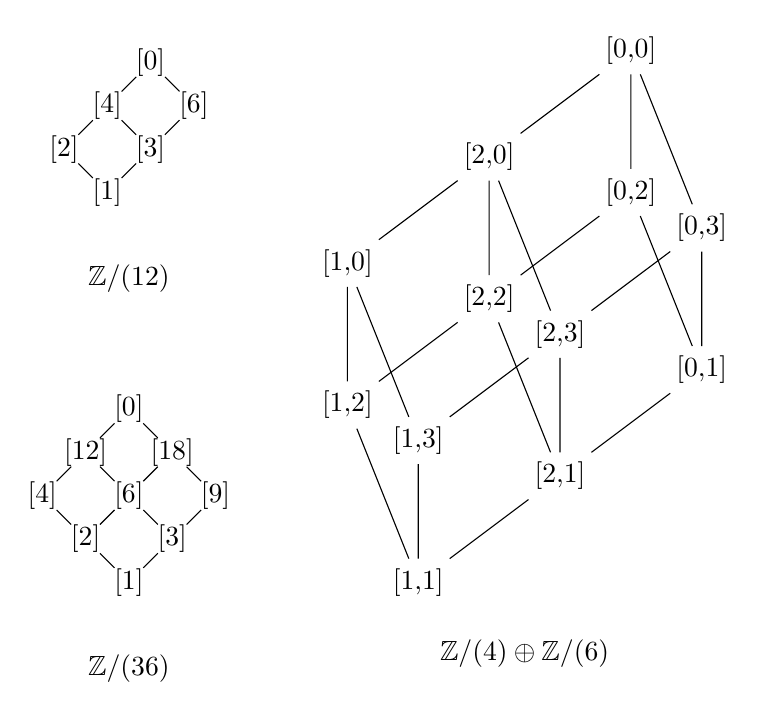
\begin{tikzpicture}
  \begin{scope}[scale=0.55,shift={(0,9)},vtx/.style={inner sep=0}]
    \node[vtx,align=center] (1) at (1,0) {\([1]\)};
    \node[vtx,align=center] (2) at (0,1) {\([2]\)};
    \node[vtx,align=center] (3) at (2,1) {\([3]\)};
    \node[vtx,align=center] (4) at (1,2) {\([4]\)};
    \node[vtx,align=center] (6) at (3,2) {\([6]\)};
    \node[vtx,align=center] (0) at (2,3) {\([0]\)};
    \draw[-] (1) -- (2) -- (4) -- (0) -- (6) -- (3) -- (4);
    \draw[-] (1) -- (3);
    \node (label) at (1.5,-2) {\(\ZZ/(12)\)};
  \end{scope}

  \begin{scope}[scale=0.55,shift={(0.5,0)},vtx/.style={inner sep=0}]
    \node[vtx,align=center] (1)  at (1,0) {\([1]\)};
    \node[vtx,align=center] (2)  at (0,1) {\([2]\)};
    \node[vtx,align=center] (3)  at (2,1) {\([3]\)}; 
    \node[vtx,align=center] (4)  at (-1,2) {\([4]\)};
    \node[vtx,align=center] (6)  at (1,2)  {\([6]\)};
    \node[vtx,align=center] (9)  at (3,2)  {\([9]\)};
    \node[vtx,align=center] (12) at (0,3) {\([12]\)};
    \node[vtx,align=center] (18) at (2,3) {\([18]\)};
    \node[vtx,align=center] (0)  at (1,4) {\([0]\)};
    \draw[-] (1) -- (2) -- (4) -- (12) -- (0) -- (18) -- (6) -- (12);
    \draw[-] (18) -- (9) -- (3) -- (6) -- (2);
    \draw[-] (1) -- (3);
    \node[align=center] (label) at (1,-2) {\(\ZZ/(36)\)};
  \end{scope}

  \begin{scope}[scale=0.45,shift={(8,0)}]
    \coordinate (O) at (0,0);
    \node[align=center] (11) at (2,0)   {\([1,\!1]\)};
    \node[align=center] (12) at (0,5)   {\([1,\!2]\)};
    \node[align=center] (13) at (2,4)   {\([1,\!3]\)};
    \node[align=center] (10) at (0,9)   {\([1,\!0]\)};
    \node[align=center] (21) at (6,3)   {\([2,\!1]\)};
    \node[align=center] (22) at (4,8)   {\([2,\!2]\)};
    \node[align=center] (23) at (6,7)   {\([2,\!3]\)};
    \node[align=center] (20) at (4,12)  {\([2,\!0]\)};
    \node[align=center] (01) at (10,6)  {\([0,\!1]\)};
    \node[align=center] (02) at (8,11)  {\([0,\!2]\)};
    \node[align=center] (03) at (10,10) {\([0,\!3]\)};
    \node[align=center] (00) at (8,15)  {\([0,\!0]\)};
    \draw[-] (11) -- (12) -- (10) -- (13) -- (11);
    \draw[-] (21) -- (22) -- (20) -- (23) -- (21);
    \draw[-] (01) -- (02) -- (00) -- (03) -- (01);
    \draw[-] (11) -- (21) -- (01);
    \draw[-] (12) -- (22) -- (02);
    \draw[-] (13) -- (23) -- (03);
    \draw[-] (10) -- (20) -- (00);
    \node[align=center] (label) at (5,-2) {\(\ZZ/(4) \oplus \ZZ/(6)\)};
  \end{scope}
\end{tikzpicture}
\end{center}
\caption{\label{fig:divisor-diagrams} Some divisor diagrams.}
\end{figure}

Even if the divisor diagram of \(R\) is infinite it may be helpful to see small parts of it at a time.
If \(a \in R\) is an element, the divisor diagram of \(a\) in \(R\) is simply the hasse diagram of the divisors of \(a\).
Divisor diagrams provide an important answer to what we might call the Visualization Problem.
\begin{titlebox}{The Visualization Problem}
\begin{center}
Given a ring, can we draw a picture of it?
\end{center}
\end{titlebox}
In addition to divisor diagrams both cayley tables and commutative diagrams are also useful visualization tools, and we will see others.
For infinite rings, or even just large finite rings, the complete divisor diagram may not be very helpful.
But even just looking at a portion of the diagram can give insight.
Seeing a ring in this way can also lead us to make conjectures.
For instance, perhaps \(R\) is infinite, but \(\ASSOCLAT{R}\) is finite, or has only finite ``height'', or ``width'' (whatever that means), or has only finitely many minimal or maximal elements. Does that imply anything about \(R\)?
Do divisor diagrams always have the boxy shape of the examples in Figure \ref{fig:divisor-diagrams}?



%---------%
\Exercises%
%---------%

\begin{exercise}
Compute the associate classes of \(\ZZ\).
\end{exercise}


\begin{exercise}
Draw the divisor diagrams of the following rings.
\begin{proplist*}
\item \(\ZZ/(8)\)
\item \(\POW{\{a,b,c\}}\)
\item \(\ZZ/(4) \oplus \ZZ/(4)\)
\item \(\ZZ/(36)\)
\end{proplist*}
\end{exercise}


\begin{exercise}
Show that \(R\) is a field precisely when \(\ASSOCLAT{R}\) consists only of \([0]\) and \([1]\).
\end{exercise}


\begin{exercise}
(@@@) find a CU nondomain and \(a\), \(b\) where \(a|b\) and \(b|a\) but \(a\), \(b\) not associate.
\end{exercise}


\begin{exercise}
Show that divisibility on \(\ZZ/(4)\) is symmetric.
\end{exercise}


\begin{exercise}
Let \(R\) be a domain.
Show that \(a \in R\) is irreducible if and only if \([a]\) is \(\lesssim\)-minimal.
\end{exercise}


\begin{exercise} \label{exerc:assoc-prod}
Let \(R\) be a CU ring.
We define a kind of setwise product on associate classes as follows: given \(A,B \in \ASSOCLAT{R}\), we define \[ A \ast B = \{ ab \mid a \in A, b \in B \}. \]
Show that the following hold.
\begin{proplist*}
\item \(A \ast B \in \ASSOCLAT{R}\), so that \(\ast\) is a binary operation on \(\ASSOCLAT{R}\).
\item \((A \ast B) \ast C = A \ast (B \ast C)\) for all \(A,B,C \in \ASSOCLAT{C}\).
\item \(A \ast B = B \ast A\) for all \(A,B \in \ASSOCLAT{R}\).
\item \label{exerc:assoc-prod:cancel} If \(R\) is a domain and \(A \ast C = B \ast C\), then \(A = B\).
\end{proplist*}
\end{exercise}


\begin{dfn}[Monotone Map]
Recall that a \emph{preorder} is a set \(P\) equipped with a relation \(\lesssim\) which is reflexive and transitive.
If \(P\) and \(Q\) are preorders, a mapping \(\varphi : P \rightarrow Q\) is called \emph{monotone}\index{monotone} if whenever \(a \lesssim b\) in \(P\) we have \(\varphi(a) \lesssim \varphi(b)\) in \(Q\).
Similarly, we say \(\varphi\) is \emph{antitone} if whenever \(a \lesssim b\) in \(P\) we have \(\varphi(b) \lesssim \varphi(a)\) in \(Q\).
\end{dfn}


\begin{exercise}
Let \(R\) be a CU ring.
\begin{proplist*}
\item Show that \(R\) is a preorder under the divisibility relation.
\item Show that the mapping \(\varphi : R \rightarrow \ASSOCLAT{R}\) given by \(\varphi(r) = [r]\) is a preorder homomorphism.
\end{proplist*}
\end{exercise}


\begin{exercise}
Let \(\varphi : R \rightarrow S\) be a ring homomorphism, where \(R\) and \(S\) are commutative.
Show that, if we consider \(R\) and \(S\) to be preorders under divisibility, then \(\varphi\) is monotone.
\end{exercise}


\begin{exercise}
Let \(\varphi : R \rightarrow S\) be a unital ring homomorphism.
\begin{proplist}
\item Show that if \(a,b \in R\) and \(a \ASSOC b\), then \(\varphi(a) \ASSOC \varphi(b)\).
\item Show that the relation \( \Phi \subseteq \ASSOCLAT{R} \times \ASSOCLAT{S} \) given by \[ \Phi = \{ ([a],[\varphi(a)]) \mid a \in R \} \] is well-defined and total.
\item Show that \(\Phi\) is monotone.
\item Show that if \(\varphi\) is surjective, then \(\Phi\) is surjective.
\end{proplist}
\end{exercise}

      \newpage

    \section{Greatest Common Divisors and GCD Rings}
      \label{sec:gcd-rings}
      In \(\ZZ\) any two elements have a greatest common divisor, and this concept turns out to have some interesting uses.
We generalize GCDs to arbitrary CU rings as follows.

\begin{dfn}[Greatest Common Divisor]
Let \(R\) be a CU ring with \(a,b \in R\).
We say \(d \in R\) is a \emph{greatest common divisor}\index{greatest common divisor} of \(a\) and \(b\) if the following hold.
\begin{proplist}
\item \(d\) is a \emph{common divisor}\index{common divisor} of \(a\) and \(b\); that is, \(d|a\) and \(d|b\).
\item \(d\) is greatest among the common divisors of \(a\) and \(b\); that is, if \(c \in R\) such that \(c|a\) and \(c|b\), then \(c|d\).
\end{proplist}
The set of all greatest common divisors of \(a\) and \(b\) is denoted \(\GCD{a}{b}\).
We say that \(a\) and \(b\) are \emph{relatively prime}\index{relatively prime}, denoted \(a \COPRIME b\), if \(1_R \in \GCD{a}{b}\).
\end{dfn}

Watch out: sometimes in \(\ZZ\) the greatest common divisor is defined to be the \emph{largest} common divisor with respect to the \(\leq\) relation.
But in an arbitrary domain we may not have a meaningful order relation, so the word ``largest'' is interpreted here with respect to divisibility.
An important consequence of this is that in a general domain, greatest common divisors need not exist, and if they do, they need not (and generally won't) be unique.
For example by our definition we have \(\GCD{4}{6} = \{2, -2\}\) in \(\ZZ\).

\begin{prop} \label{prop:gcd-assoc}
Let \(R\) be a domain with \(a,b,c \in R\).
Then we have the following.
\begin{proplist*}
\item \label{prop:gcd-assoc:class}\(\GCD{a}{b}\) is either empty or an associate class.
\item \label{prop:gcd-assoc:well-defined} If \(a \ASSOC b\), then \(\GCD{a}{c} = \GCD{b}{c}\).
\end{proplist*}
\end{prop}

\begin{proof}
\begin{inlineproplist}
\item Let \(a,b \in R\) and suppose \(\GCD{a}{b}\) is not empty; say \(x\) is a greatest common divisor of \(a\) and \(b\).
It suffices to show that if \(y \ASSOC x\), then \(y\) is also a greatest common divisor of \(a\) and \(b\).
By \eref{exerc:associate-divides} we have that \(y|a\) and \(y|b\), and if \(c|a\) and \(c|b\), then \(c|x\), so that \(c|y\) by \eref{exerc:associate-divides}.
\item Say \(b = ua\), and suppose we have \(d \in \GCD{a}{c}\).
Now \(d|a\), so that \(d|b\) by \eref{exerc:associate-divides}.
That is, \(d\) is a common divisor of \(b\) and \(c\).
Suppose now that \(e|b\) and \(e|c\).
We have \(e|a\) by \eref{exerc:associate-divides}, so that \(e|d\).
Thus \(d \in \GCD{b}{c}\).
Similarly, if \(d \in \GCD{b}{c}\) then \(d \in \GCD{a}{c}\).
That is, if \emph{either} \(\GCD{a}{c}\) or \(\GCD{b}{c}\) is nonempty, then the two are equal.
\end{inlineproplist}
\end{proof}

It is important to remember that \(\GCD{\ast}{\ast}\) is a \emph{subset} of \(R\), not a specific element.
However, \propref{prop:gcd-assoc} says that nonempty GCDs are associate classes, and that GCD cannot distinguish elements in the same associate class.
This suggests that we should really think of \(\GCD{\ast}{\ast}\) as a binary operation on the associate classes of \(R\); this is explored further in \eref{exerc:gcd-meet}.

In \(\ZZ\), we had some nice technology for computing GCDs -- namely, the Euclidean Algorithm.
In an arbitrary domain the situation is not so nice; computing \(\GCD{a}{b}\) is generally difficult.
The next proposition handles some special cases.

\begin{prop} \label{prop:gcd-basics}
Let \(R\) be a domain with \(a,b \in R\).
Then we have the following.
\begin{proplist*}
\item \(\GCD{a}{b} = \GCD{b}{a}\).
\item \(a|b\) if and only if \(a \in \GCD{a}{b}\).
\item \(a \in \GCD{a}{0}\).
\item If \(u \in R\) is a unit then \(a \COPRIME u\).
\item \label{prop:gcd-basics:coprime-factor} If \(a \COPRIME b\) and \(c|a\), then \(c \COPRIME b\).
\end{proplist*}
\end{prop}

\begin{proof}
\begin{inlineproplist}
\item Follows from the definition of GCD.
\item Suppose \(a|b\).
Now \(a|a\) and \(a|b\), so \(a\) is a common divisor of \(a\) and \(b\).
Moreover if \(c|a\) and \(c|b\), then \(c|a\), so \(a\) is a greatest common divisor of \(a\) and \(b\).
The converse follows from the definition of common divisor.
\item Note that \(a|a\) and \(a|0\) by \ref{prop:divides-basics}, so \(a\) is a common divisor of \(a\) and \(0\).
Certainly if \(c|a\) and \(c|0\) then \(c|a\), as needed.
\item It suffices to show that \(1_R\) is a greatest common divisor of \(a\) and \(u\).
Certainly \(1_R|a\) and \(1_R|u\).
Now if \(c|a\) and \(c|u\), then \(c\) is a unit by \sref{prop:divides-basics}{unit-div}, and thus \(c|1_R\) as needed.
\item If \(x \in \GCD{c}{b}\), then we have \(x|a\) and \(x|b\), so that \(x|1_R\) as needed.
\end{inlineproplist}
\end{proof}

The next result is very important: it roughly says that if \(a\) divides a product but is relatively prime to one of the factors, then it must divide the other factor.

\begin{prop}[Euclid's Lemma]\label{prop:euclids-lemma}\index{Euclid's Lemma}
Let \(R\) be a domain with \(a,b,c \in R\).
\begin{proplist*}
\item \label{prop:euclids-lemma:dist} If \(d \in \GCD{a}{b}\) and \(e \in \GCD{ac}{bc}\) then \(e \ASSOC dc\).
\item \label{prop:euclids-lemma:stmt} If \(a \COPRIME b\), \(\GCD{ac}{bc}\) exists, and \(a|bc\), then \(a|c\).
\end{proplist*}
\end{prop}

\begin{proof}
\begin{inlineproplist}
\item Note that \(d|a\) and \(d|b\), so that \(dc|ac\) and \(dc|bc\), and thus \(dc|e\).
Say \(e = dcx\).
Now \(dcx|ac\) and \(dcx|bc\), so that \(dx|a\) and \(dx|b\).
Now \(dx|d\), so that \(x|1_R\).
That is, \(x\) is a unit, and we have \(e \ASSOC dc\).
\item Say \(e \in \GCD{ac}{bc}\).
Now \(a|ac\) and \(a|bc\), so \(a|e\).
By \ref{prop:euclids-lemma:dist}, we have \(e \ASSOC c\), thus \(a|c\) as needed.
\end{inlineproplist}
\end{proof}

In fact many nice properties hold for greatest common divisors, all of which are contingent on GCDs existing in the first place -- and this is not guaranteed!
That is, there are some domains, like \(\ZZ\), where \(\GCD{a}{b}\) is always nonempty, but there are other domains containing elements which do not have any greatest common divisors.
(We explore some examples in the exercises.)
Those rings, like \(\ZZ\), where GCDs always exist are special enough to warrant a definition.

\begin{dfn}[GCD Ring] \label{dfn:gcd-ring}
Let \(R\) be a domain.
We say that \(R\) is a \emph{GCD ring}\index{GCD ring} if any two elements of \(R\) have a greatest common divisor.
If \(R\) is also a domain, we say it is a \emph{GCD domain}\index{GCD domain}.
\end{dfn}

Of course our motivating example \(\ZZ\) is a GCD domain, and we will see many more.
First, we establish that several of the nice things we can say about GCDs in \(\ZZ\) hold in an arbitrary GCD domain.

\begin{prop} \label{prop:gcd-dom-basics}
Let \(R\) be a GCD domain with \(a,b,c \in R\).
\begin{proplist*}
\item If \(a \COPRIME b\) and \(a \COPRIME c\), then \(a \COPRIME bc\).
\item \label{prop:gcd-dom-basics:drop-factor} If \(a \COPRIME b\), then \(\GCD{a}{bc} = \GCD{a}{c}\).
\item If \(d \in \GCD{a}{b}\) with \(a = dx\) and \(b = dy\), then \(x \COPRIME y\).
\item If \(a \COPRIME b\), \(d \in \GCD{ab}{c}\), \(e \in \GCD{a}{c}\), and \(f \in \GCD{b}{c}\), then \(d \ASSOC ef\).
\end{proplist*}
\end{prop}

\begin{proof}
\begin{inlineproplist}
\item Suppose \(d|a\) and \(d|bc\).
Now \(d|ab\) and \(d|cb\), so that \(d|e\), where \(e \in \GCD{ab}{cb}\).
By \sref{prop:euclids-lemma}{dist} we have that \(e|b\).
But now \(e|a\) and \(e|b\), so that \(e|1_R\); thus \(1_R\) is a greatest common divisor of \(a\) and \(bc\).
\item Let \(d \in \GCD{a}{bc}\) and \(e \in \GCD{a}{c}\); it suffices to show that \(d \ASSOC e\).
To this end, note that \(e|a\) and \(e|c\), so that \(e|bc\); thus \(e|d\).
Now \(d|a\), so that \(d|ac\), and \(d|bc\).
Letting \(f \in \GCD{ac}{bc}\), we have \(f \ASSOC 1_R \cdot c\), and thus \(d|c\).
So we have \(d|e\), and thus \(d \ASSOC e\) as needed.
\item Let \(e \in \GCD{x}{y}\).
Now by \sref{prop:euclids-lemma}{dist} we have \(d \ASSOC ed\), and thus \(1_R \ASSOC e\) by \sref{prop:div-domain}{assoc-cancel}, as needed.
\item Say \(a = ex\) and \(c = ey\) where \(x \COPRIME y\).
Note that \(b \COPRIME e\) by \sref{prop:gcd-basics}{coprime-factor}, so that \[ \GCD{b}{c} = \GCD{b}{ey} = \GCD{b}{y} = \GCD{xb}{y} \] by \sref{prop:gcd-dom-basics}{drop-factor}.
In particular, we have \(d \ASSOC ef\) by \sref{prop:euclids-lemma}{dist}.
\end{inlineproplist}
\end{proof}

Recall that in a general domain we can characterize the ``indivisible'' elements in two slightly different ways: the irreducibles and the primes.
In any domain, every prime is also irreducible.
In a GCD domain, the converse also holds.

\begin{prop} \label{prop:gcd-irreducible-implies-prime}
If \(R\) is a GCD domain, then every irreducible element of \(R\) is also prime.
\end{prop}

\begin{proof}
Let \(p\) be irreducible and suppose \(p|ab\).
Let \(d \in \GCD{a}{p}\), and write \(a = da'\) and \(p = dp'\).
Since \(p\) is irreducible, either \(d\) or \(p'\) is a unit.
If \(d\) is a unit, then we have \(p|b\) by Euclid's Lemma.
If \(p'\) is a unit, then \(p|a\).
\end{proof}

Remember that unlike \(\ZZ\), in a GCD domain we only know that greatest common divisors \emph{exist} -- we don't necessarily have a way to actually compute them.
In the exercises we will compute GCDs (@@@)



%---------%
\Exercises%
%---------%

\begin{exercise}
Let \(R\) and \(S\) be domains, and let \(x,y \in R \oplus S\).
Show that if \(x|y\) and \(y|x\) then \(x \ASSOC y\).
\end{exercise}

\begin{exercise}
Let \(R\) and \(S\) be GCD domains with \(r_1,r_2 \in R\) and \(s_1,s_2 \in S\), and let \(d_r \in \GCD{r_1}{r_2}\) and \(d_s \in \GCD{s_1}{s_2}\).
Show that \((d_r, d_s) \in \GCD{(r_1,s_1)}{(r_2,s_2)}\).
\end{exercise}

\begin{exercise}
Let \(X\) be a nonempty set and let \(a,b \in \POW{X}\).
Show that if \(a|b\) and \(b|a\) then \(a = b\).
\end{exercise}

\begin{exercise}
Let \(X\) be a nonempty set, and let \(A, B \in \POW{X}\).
Show that \(A \cup B \in \GCD{A}{B}\).
\end{exercise}

\begin{exercise}
(@@@) Let \(n > 1\).
\begin{proplist*}
\item Show that \(k \ASSOC \GCD{k}{n}\).
\item Show that the associate classes of \(\ZZ/(n)\) are of the form \(\GCD{k}{n}\) for \(0 \leq k < n\).
\item Show that if \(a|b\) and \(b|a\) then \(a \ASSOC b\).
\end{proplist*}
\end{exercise}

\begin{exercise}[\(\ZZ/(n)\) has greatest common divisors.]
(@@@) Let \(n > 1\), let \(a,b \in \ZZ/(n)\), and let \(d\) be the greatest common divisor of \(a\), \(b\), and \(n\) in \(\ZZ\).
Show that \(d \in \GCD{a}{b}\) in \(\ZZ/(n)\).
\end{exercise}

\begin{exercise}
(@@@) find an example of two ring elements which divide each other but are not associate.
\end{exercise}

\begin{exercise} \label{exerc:gcd-meet}
Let \(R\) be a CU ring, and let \(\ASSOCLAT{R}\) be the set of \(\ASSOC\)-equivalence classes of \(R\) (see \ref{dfn:assoc-sld}).
Define a relation \(\wedge \subseteq (\ASSOCLAT{R} \times \ASSOCLAT{R}) \times \ASSOCLAT{R}\) as follows.
\[ \wedge = \left\{ \left(([a],[b]), \GCD{a}{b}\right) \mid a,b \in R\ \mathrm{such\ that}\ \GCD{a}{b} \neq \varnothing \right\}. \]
\begin{proplist}
\item Show that \(\wedge\) is well-defined.
\item Show that \(\wedge\) is total if and only if \(R\) is a GCD domain.
\end{proplist}
That is, \(\wedge\) is a partial function \(\ASSOCLAT{R} \times \ASSOCLAT{R} \rightarrow \ASSOCLAT{R}\) which is total if and only if \(R\) is a GCD domain.
\end{exercise}

\begin{exercise}
Let \(R\) be a GCD domain, and let \(\wedge\) be defined on \(\ASSOCLAT{R}\) as in \eref{exerc:gcd-meet}.
Show that the following hold for all \(A,B,C \in \ASSOCLAT{R}\).
\begin{proplist*}
\item \(A \wedge A = A\)
\item \(A \wedge B = B \wedge A\)
\item \((A \wedge B) \wedge C = A \wedge (B \wedge C)\)
\end{proplist*}
\end{exercise}

\begin{exercise}[A domain which is not a GCD domain.] In this exercise we will show that \(\ZZ[\sqrt{-3}]\) is a domain which is not a GCD domain.
\begin{proplist}
\item Show that the equation \(a^2 + ab + b^2 = 2\) has no solutions in \(\ZZ\).
\item Show that no element of \(\ZZ[\sqrt{-3}]\) has norm 2 (@@@).
\item Show that 2 is irreducible in \(\ZZ[\sqrt{-3}]\).
\item Show that 2 divides \(4 = (1 + \sqrt{-3})(1 - \sqrt{-3})\) in \(\ZZ[\sqrt{-3}]\), but that 2 does not divide \(1 + \sqrt{-3}\) or \(1 - \sqrt{-3}\).
In particular, 2 is not prime in \(\ZZ[\sqrt{-3}]\).
\item Conclude that \(\ZZ[\sqrt{-3}]\) is not a GCD domain.
\end{proplist}
\end{exercise}

\begin{dfn}[Least Common Multiple]
Let \(R\) be a domain, with \(a,b \in R\).
We say that \(m \in R\) is a \emph{least common multiple}\index{least common multiple} of \(a\) and \(b\) in \(R\) if the following hold.
\begin{proplist}
\item \(m\) is a \emph{common multiple}\index{common multiple} of \(a\) and \(b\); that is, \(a|m\) and \(b|m\).
\item \(m\) is least among the common multiples of \(a\) and \(b\); that is, if \(n \in R\) such that \(a|n\) and \(b|n\), then \(m|n\).
\end{proplist}
The set of all least common multiples of \(a\) and \(b\) is denoted \(\LCM{a}{b}\).
\end{dfn}

\begin{exercise}
(@@@) example where euclid's lemma fails
\end{exercise}

\begin{exercise}
(@@@) Show that \(\ZZFRAC{k}\) is a GCD domain.
\end{exercise}

\begin{exercise}
(@@@) is this true: if \(R\) is a domain in which every irreducible is prime, then \(R\) is a GCD domain.
\end{exercise}

      \newpage

    \section{Factorization and UFDs}
      \label{sec:ufds}
      In \(\ZZ\) we have the Fundamental Theorem of Arithmetic: every integer can be written as a product of prime integers in essentially one way, in the sense that any two factorizations have the same length and can be rearranged so that corresponding factors are associate.
For example,

\[ 30 = (-2) \cdot 5 \cdot (-3) \quad \mathrm{and} \quad 30 = 3 \cdot (-5) \cdot (-2) \] are different factorizations of 30, but we can rearrange them as \[ 30 = (-2) \cdot (-3) \cdot 5 \quad \mathrm{and} \quad 30 = (-2) \cdot 3 \cdot (-5), \] where \(-2\) and \(-2\) are associate, \(-3\) and 3 are associate, and 5 and \(-5\) are associate.

FTA is merely a statement about the \emph{existence} of these unique factorizations, but if we examine the usual proof, we see that it can be turned into an effective algorithm which actually finds a factorization.
The most basic (but correct!) algorithm to actually \emph{compute} the prime factorization of a given integer \(n\) goes something like this.

\begin{framed}
\noindent To find a prime factorization of \(n\):

Search among all \(a\) with \(1 < a < |n|\) for a divisor of \(n\).
\begin{itemize}
\item If no such divisor is found, then \(n\) is prime and thus \(n = n\) is a prime factorization of \(n\).
\item If such a divisor is found, with \(n = ab\), then \emph{recursively} find prime factorizations \(a = p_1 \cdots p_h\) and \(b = q_1 \cdots q_k\).
Then \(n = p_1 \cdots p_h q_1 \cdots q_k\) is a prime factorization of \(n\).
\end{itemize}
\end{framed}

There are some minor optimizations we can make to this procedure, say by only looking for \emph{prime} divisors up to \(\sqrt{n}\).
In the end this \textbf{trial division} procedure is slow, but correct.

We might try to generalize this procedure to any domain by replacing the word ``prime'' with ``irreducible''.
However, there are many subtle ways it can fail.
For a particular domain \(R\) and a particular element \(x \in R\),
\begin{itemize}
\item Maybe there is no way to restrict the possible divisors of \(x\) to a finite list of candidates.
\item Maybe \(R\) has no irreducible elements.
\item Maybe \(R\) does have irreducible elements, but the factorization procedure never terminates.
(Every ``factorization'' of \(x\) has infinite length.)
\item Maybe the factorization procedure terminates only for \emph{some} choices of the divisors \(a\) and \(b\).
(Some ``factorizations'' of \(x\) have infinite length.)
\item Maybe the factorization procedure always terminates, but \(x\) has arbitrarily long factorizations.
\item Maybe the factorizations of \(x\) are all of bounded length, but generally have \emph{different} lengths.
\item Maybe the factorizations of \(x\) are all of the same length, but cannot generally be rearranged so that corresponding factors are associates.
\end{itemize}

By the way, there are examples of domains where each of these things happens! Evidently, then, a ring like \(\ZZ\) where the Fundamental Theorem of Arithmetic holds is very special, since it manages to avoid all these problems.
We single out rings with unique factorization with a definition.

\begin{dfn}[Unique Factorization Domain] \label{dfn:ufd}
Let \(R\) be a domain.
We say that \(R\) is a \emph{unique factorization domain}\index{UFD} (UFD) if every nonzero element of \(R\) can be written as a finite product of irreducibles in essentially one way.

More precisely, for each \(x \in R\), we have \(x = p_1 p_2 \cdots p_m\) where each \(p_i\) is irreducible, and if \(x = q_1 q_2 \cdots q_\ell\), for some irreducible \(q_i\), then \(m = \ell\) and there is a permutation \(\sigma\) of \(\{1, \ldots, m\}\) so that \(p_i\) and \(q_{\sigma(i)}\) are associates for each \(i\).
\end{dfn}

Of course \(\ZZ\) is our prototypical example of a UFD.
The value of a UFD is that irreducibles act like the ``building blocks'' for all other elements, much like the prime numbers are the building blocks of the integers.
For instance, irreducible factorizations give us a nice characterization of divisibility as follows.

\begin{prop} \label{prop:divisibility-in-a-ufd}
Let \(R\) be a UFD, and let \(x, y \in R\).
Suppose we have factored \(x\) and \(y\) as \[ x = p_1^{e_1} p_2^{e_2} \cdots p_m^{e_m} \quad \mathrm{and} \quad y = up_1^{f_1} p_2^{f_2} \cdots p_m^{f_m}, \] where the \(e_i\) and \(f_i\) are natural numbers.
(Note that this is always possible by taking associates and letting \(e_i\) or \(f_i\) be zero in case some irreducible does not appear in the factorization of \(x\) or \(y\).) Then \(x|y\) if and only if \(e_i \leq f_i\) for each \(i \in [1,m]\).
\end{prop}

\begin{proof}
(@@@)
\end{proof}

From here, we can characterize gcds nicely.

\begin{prop} \label{prop:ufd-implies-gcd-domain}
Every UFD is a GCD Domain.
Specifically, if \(R\) is a UFD and \(x, y \in R\) such that \[ x = p_1^{e_1} p_2^{e_2} \cdots p_m^{e_m} \quad \mathrm{and} \quad y = up_1^{f_1} p_2^{f_2} \cdots p_m^{f_m}. \] Then \[ z = p_1^{\min(e_1,f_1)} p_2^{\min(e_2,f_2)} \cdots p_m^{\min(e_m,f_m)} \] is a maximal common divisor of \(x\) and \(y\).
\end{prop}

Unique factorization is a very natural thing to want in a ring.
In many areas of mathematics, one way to try to understand some object is to decompose it into smaller pieces in a simple way, understand the smaller pieces, and then reassemble into an understanding of the original object.
It is especially nice, then, if there is \emph{only one way} that the decomposition process could proceed.
UFDs are very rare, but fortunately many rings of practical importance (such as \(\ZZ\)) do have unique factorization.

One of the historical threads that led to the development of modern abstract algebra was an attempt by 19th century mathematician Ernst Kummer to prove Fermat's Last Theorem using factorization.
Recall that FLT is the assertion that the equation \(a^n + b^n = c^n\) has no interesting integer solutions \((a,b,c)\) if \(n > 2\).
Kummer's idea was to rearrange this equation as \(a^n = c^n - b^n\).
Now if \(\zeta\) is a primitive \(n\)th root of unity, the right hand side factors as \[ a^n = (c - b)(c - \zeta b)(c - \zeta^2 b) \cdots (c - \zeta^{n-1} b). \] For example, if \(n = 4\) then \(i\) is a primitive 4th root of unity and we have \[ a^4 = (c - b)(c - ib)(c + b)(c + ib) \] This yields two different factorizations of \(a^n\), which may lead to a contradiction.

The problem with Kummer's idea was that it only works if the ring \(\ZZ[\zeta]\) is a UFD, which, at the time, was not known.
Nobody had bothered to check!
The idea that this line of attack might solve the famous FLT led to an explosion of new ideas in algebraic number theory that continues to this day.

Eventually it was found that \(\ZZ[\zeta]\) is sometimes a UFD, but not always -- so Kummer's idea did not work.
But it is more useful to judge an idea not by what problems it \emph{can't} solve, but by what problems it \emph{can} and what new ideas it inspires.
By this measure Kummer's attempt at FLT is among the most successful failures in mathematics.



%---------%
\Exercises%
%---------%

\begin{exercise}
Suppose that \(R\) is a domain and \(N : R \rightarrow \NN\) a multiplicative norm.
Show that if \(x \in R\), then the irreducible factorizations of \(x\) have bounded length.
\end{exercise}

\begin{dfn}
Let \(R\) be a domain and \(p,x \in R\), with \(x \neq 0\).
We define the \(p\)-divisibility order of \(x\), denoted \(\DIVORD{p}{x}\), to be the exponent of the largest power of \(p\) which divides \(x\) (if it exists).
That is, \(\DIVORD{p}{x} = \max \{ k \mid p^k | x \}\) if this set has a maximum and is undefined otherwise.
\end{dfn}

\begin{exercise}
Let \(R\) be a UFD.
\begin{proplist}
\item Show that \(\DIVORD{p}{x}\) exists for all \(p,x \in R\) with \(x \neq 0\).
\item Show that if \(p\) is irreducible, then \(\DIVORD{p}{ab} = \DIVORD{p}{a} + \DIVORD{p}{b}\) for all \(a,b \in R\).
\item Show that \(N : R \rightarrow \NN\) given by \(N(x) = 2^{\DIVORD{p}{x}}\) if \(x \neq 0_R\) and \(0\) if \(x = 0_R\) is a multiplicative norm on \(R\).
\end{proplist}
\end{exercise}

      \newpage

    \section{Division with Remainder and Euclidean Domains}
      \label{sec:eds}
      In \(\ZZ\), we had the extremely important Division Algorithm. This theorem states that if \(a\) and \(b\) are integers with \(b \neq 0\), then there exists a ``quotient'' \(q\) and a ``remainder'' \(r\) such that \(a = qb + r\), and, moreover, the remainder is not too large -- \(0 \leq r < |b|\). This is the result from which most of the interesting results and algorithms in \(\ZZ\) spring.

We'd like to generalize this property to integral domains. Notice that one problem is the appearance of absolute value in the bound on \(r\): in general, rings do not have anything like absolute value, or a way to compare the ``sizes'' of two elements. However in \autoref{sec:norms} we did describe such a gadget for some rings: norms. Recall that a map \(N : R \rightarrow \NN\) is called a \emph{norm} if (1) \(N(x) = 0\) iff \(x = 0\) and (2) \(N(xy) \geq N(x)\) when \(y \neq 0\). These properties do generalize the absolute value.

\begin{dfn}[Euclidean Norm]
Let \(R\) be a domain and \(N : R \rightarrow \NN\) a norm.
\begin{proplist}
\item We say that \(N\) is \emph{Euclidean} if for all \(a,b \in R\) with \(b \neq 0\), there exist \(q,r \in R\) such that \(a = qb+r\) and \(0 \leq N(r) < N(b)\).
\item A domain which has a Euclidean norm is called a \emph{Euclidean Domain}.
\end{proplist}
\end{dfn}

Of course \(\ZZ\) is a Euclidean Domain with norm \(N(a) = |a|\). The existence of a Euclidean norm on \(R\) is very powerful. For instance, many of the nice properties of \(\ZZ\) which we derived from the Division Algorithm have analogues in any Euclidean Domain. More generally, the norm allows us to recover some of the benefits of mathematical induction.

\begin{prop}
Every Euclidean domain is a UFD.
\end{prop}

\begin{proof}
(@@@)
\end{proof}

As a consequence of this result, every Euclidean domain is also a GCD domain; recall that we have a nice characterization of greatest common divisors in a UFD due to unique factorization. But this characterization of GCDs is \emph{nonconstructive}; we know that given two elements of a UFD, they have a greatest common divisor, but actually computing a GCD requires that we be able to factor and recognize associates. In a Euclidean domain, we can do much better.

\begin{prop}[Euclidean Algorithm] \label{prop:euclidean-algorithm}
Every Euclidean Domain is also a GCD Domain.
\end{prop}

\begin{proof}
Let \(R\) be a Euclidean domain with norm \(N\). We want to show that for all \(a \in R\), for all \(b \in R\), the set \(\GCD{a}{b}\) is not empty. We proceed by strong induction on \(N(a)\).

\textbf{Base case.} If \(N(a) = 0\), then \(a = 0\), and so we have \(b \in \GCD{a}{b}\) for all \(b\).

\textbf{Inductive Step.} Let \(a \in R\) and suppose that the result holds for all \(a'\) with \(1 \leq N(a') < N(a)\). In particular, note that \(a \neq 0\). Now let \(b \in R\). By the division algorithm we may decompose \(b\) as \(b = qa + r\), where \(0 \leq N(r) < N(a)\). If \(r = 0\) then \(a|b\) and we have \(a \in \GCD{a}{b}\). If \(r \neq 0\), then by the inductive hypothesis \(\varnothing \neq \GCD{r}{a} = \GCD{b-qa}{a} = \GCD{b}{a}\) as needed.
\end{proof}

Again, the proof of this statement is logically redundant; we already knew that Euclidean domains are GCD domains. But algorithmically this proof gives us something very strong. If we have an effective procedure for computing quotients and remainders in \(R\), then we have an effective procedure for computing GCDs.

\begin{prop}
Every field is a Euclidean domain.
\end{prop}

\begin{proof}
Define a mapping \(N : F \rightarrow \NN\) by \(N(x) = 0\) if \(x = 0\) and 1 if \(x \neq 0\). We can see that \(N\) is a Euclidean norm.
\end{proof}




%---------%
\Exercises%
%---------%

\begin{exercise}
(@@@) (\(k\)-stage Euclidean)
\end{exercise}

\begin{exercise}
(@@@) Dropping the domain condition on euclidean domains; see \cite{samuel71}
\end{exercise}
      \newpage

    \section{Localization and the Field of Fractions}
      \label{sec:localization}
      In a general ring with 1, or even a general domain, elements typically do not have multiplicative inverses.
Those which do are called \emph{units} and are very special.
In this section we will see how a domain can be ``extended'' to a larger ring so that any given element can be made into a unit.
First we need a definition.

\begin{dfn}[Multiplicative Subset] \label{dfn:multiplicative-subset}
Let \(R\) be a domain and \(S \subseteq R\).
We say that \(S\) is a \emph{multiplicative subset}\index{multiplicative subset} (or a set of \emph{denominators}) of \(R\) if \(0 \notin R\) and if \(S\) is closed under multiplication.
\end{dfn}

Domains have plenty of multiplicative sets.
For instance, the set of all nonzero elements is multiplicative.
If \(a \in R\) is not zero, then the set \(S = \{ 1, a, a^2, a^3, \ldots \}\) of powers of \(a\) is multiplicative.
Here is the punch line of this section.

\begin{framed}
If \(S \subseteq R\) is a multiplicative subset, then we can construct a new ring, \(T\), which contains \(R\) as a subset, but in which the elements of \(S\) are units.
\end{framed}

\begin{prop}
Let \(R\) be a domain and \(S \subseteq R\) a multiplicative subset.
We define a relation \(\Phi\) on the cartesian product \(S \times R\) as follows: \[ (s_1, r_1) \Phi (s_2, r_2) \quad \mathrm{iff} \quad r_1s_2 = r_2s_1. \]
This relation \(\Phi\) is an equivalence.
\end{prop}

\begin{proof}
\begin{inlineproplist}
\item We have \(rs = rs\) for all \(r \in R\) and \(s \in S\), so that \((s,r) \Phi (s,r)\).
\item Suppose \((s_1,r_1) \Phi (s_2,r_2)\).
Then \(r_1s_2 = r_2s_1\), so that \(r_2s_1 = r_1s_2\), and thus \((s_2,r_1) \Phi (s_1,r_1)\).
\item Suppose \((s_1, r_1) \Phi (s_2, r_2)\) and \((s_2, r_2) \Phi (s_3, r_3)\).
Now \(r_1s_2 = r_2s_1\) and \(r_2s_3 = r_3s_2\).
We then have \(r_1s_2r_2s_3 = r_2s_1r_3s_2\); rearranging (since \(R\) is commutative) and using cancellation, we have \(r_1s_3 = r_3s_1\).
So \((s_1, r_1) \Phi (s_3, r_3)\) as needed.
\end{inlineproplist}
\end{proof}

Since \(\Phi\) is an equivalence, it induces a partition on the set \(S \times R\).
We will denote this quotient set \(\LOCALIZE{R}{S} = (S \times R)/\Phi\) and denote the equivalence class of \((s,r)\) by \(\frac{r}{s}\).

\begin{prop}
Let \(R\) be a domain with \(S \subseteq R\) a multiplicative subset.
Define operations \(+\) and \(\cdot\) on \(\LOCALIZE{R}{S}\) as follows.
\[ \frac{r_1}{s_1} + \frac{r_2}{s_2} = \frac{r_1s_2 + r_2s_1}{s_1s_2} \quad \mathrm{and} \quad \frac{r_1}{s_1} \cdot \frac{r_2}{s_2} = \frac{r_1r_2}{s_1s_2}. \]
Then we have the following.
\begin{proplist}
\item \(+\) and \(\cdot\) are well-defined.
\item \(\LOCALIZE{R}{S}\), with these operations, is an integral domain, which we call the \emph{localization} of \(R\) \emph{at} \(S\).
\item If \(t \in S\), then the mapping \(\iota : R \rightarrow S^{-1}R\) given by \(\iota(r) = \frac{rt}{t}\) is an injective ring homomorphism, and \(\iota(t)\) is a unit in \(S^{-1}R\).
\end{proplist}
\end{prop}

\begin{proof}
(super tedious)
\end{proof}

So \(S^{-1}R\) is a new ring which contains a ``copy'' (homomorphic image) of \(R\), within which the elements of \(S\) become units.

\begin{dfn}
Let \(R\) be a domain and let \(D = \{ x \in R \mid x \neq 0 \}\) be the multiplicative subset of all nonzero elements of \(R\).
Then the localization \(D^{-1}R\) is a field, called the \emph{field of fractions} of \(R\).
\end{dfn}

For example, \(\QQ\) is properly defined as the field of fractions of \(\ZZ\).



%---------%
\Exercises%
%---------%

\begin{exercise}
Let \(R\) be a domain and \(S,T \subseteq R\) multiplicative sets.
Show that \(ST = \{ st \mid s \in S, t \in T \}\) is multiplicative.
\end{exercise}


\begin{exercise}
Let \(R\) be a GCD domain, with \(F\) its field of fractions.
An element \(\frac{a}{b} \in F\) is said to be \emph{reduced} (or in \emph{lowest terms}) if \(\GCD{a}{b} = 1\).
\begin{proplist}
\item Show that every element of \(F\) has a reduced representative.
\item Show that reduced fractions are unique in the following sense: If \(\frac{a}{b} = \frac{c}{d}\) are both reduced, then \(c = au\) and \(d = bu\) for some unit \(u\).
\end{proplist}
\end{exercise}


\begin{exercise}
(@@@ do stuff in \(\ZZ[\frac{1}{2}]\))
\end{exercise}


\begin{exercise}
If \(R\) is a UFD and \(S \subseteq R\) any multiplicative set, then \(S^{-1}R\) is also a UFD.
\end{exercise}


\begin{exercise}
If \(R\) is a Euclidean domain and \(S \subseteq R\) any multiplicative set, then \(S^{-1}R\) is a Euclidean domain.
\end{exercise}


\begin{exercise}[Universal Property of Localization]
Let \(R\) be a ring and let \(D \subseteq R\) be a multiplicative subset.
Suppose \(\varphi : R \rightarrow S\) is a ring homomorphism (with \(S\) unital) such that \(\varphi(d)\) is a unit in \(S\) for all \(d \in D\).
Show that there is a unique ring homomorphism \(\Phi : \LOCALIZE{R}{D} \rightarrow S\) such that the following diagram commutes.
\begin{center}
\begin{tikzcd}
R \arrow[d,"\iota"] \arrow[r,"\varphi"] & S \\
\LOCALIZE{R}{D} \arrow[ur,"\Phi"] & 
\end{tikzcd}
\end{center}
That is, a unique \(\Phi\) such that \(\varphi = \Phi \circ \iota\).
\end{exercise}

      \newpage

    \section{Quadratic Numbers}
      \label{sec:quad-num}
      \begin{prop}
\(\ZZ[i]\) is a Euclidean domain under the norm \(N(a+bi) = a^2 + b^2\).
\end{prop}

\begin{proof}
Let \(\alpha = a_1 + a_2 i\) and \(\beta = b_1 + b_2 i\) be Gaussian integers, with \(\beta \neq 0\).
Thinking of \(\alpha\) and \(\beta\) as elements of \(\QQ(i)\), we have \[ \frac{\alpha}{\beta} = t_1 + t_2 i = \frac{a_1b_1 + a_2b_2}{b_1^2 + b_2^2} + \frac{a_2b_1 - a_1b_2}{b_1^2 + b_2^2} i. \] Choose integers \(q_1\) and \(q_2\) such that \(|q_1 - t_1| \leq \frac{1}{2}\) and \(|q_2 - t_2| \leq \frac{1}{2}\).
(Note that this is always possible.) Let \(\gamma = q_1 + q_2 i\), and let \(\delta = \alpha - \gamma\beta\).
Note that by construction, \(\gamma\) and \(\delta\) are in \(\ZZ[i]\).

We now have
\begin{eqnarray*}
N(\delta) & = & N(\alpha - \gamma\beta) = N\left((\frac{\alpha}{\beta} - \gamma)\beta\right) = N(\frac{\alpha}{\beta} - \gamma)N(\beta) \\
 & = & ((q_1-t_1)^2 + (q_2-t_2)^2)N(\beta) \leq \frac{1}{2}N(\beta) < N(\beta),
\end{eqnarray*}
as needed.
\end{proof}

\begin{cor}
\(\ZZ[i]\) is a GCD domain and a UFD.
\end{cor}

Here is a worked example of the division algorithm in the Gaussian integers.
Let \(\alpha = 10+7i\) and \(\beta = 3+2i\).
Now \[ \frac{\alpha}{\beta} = \frac{44}{13} + \frac{1}{13}i = (3 + \frac{5}{13}) + (0 + \frac{1}{13})i. \] Let \(t_1 = 3\) and \(t_2 = 0\), so that \(\gamma = 3\).
Now \(\delta = \alpha - \gamma\beta = 1+i\).
We then have \(10+7i = 3(3+2i) + (1+i)\) and \(N(1+i) < N(3+2i)\).


%---------%
\Exercises%
%---------%

\begin{exercise}[A Theorem of Fermat]
5 and 3 have the curious property that \(3^3 = 5^2 + 2\).
Fermat asked whether or not there are any other pairs like this: a perfect square and a perfect cube separated by 2.
(@@@)
\begin{proplist}
\item Show that \(x \equiv y \equiv 1 \pmod{2}\).
\item Show that \(x - \sqrt{-2}\) and \(x + \sqrt{-2}\) are relatively prime in (@@@).
\item Since blah is a UFD let \(x + \sqrt{-2} = (m+n\sqrt{-2})\), show that \(x = \pm 5\).
\end{proplist}
\end{exercise}

\begin{exercise}
(@@@) (Factorization in \(\ZZ[i]\))
\end{exercise}

mordell equations

      \newpage

    \phantomsection
    \section*{Summary of \autoref{chap:domains}}
      \addcontentsline{toc}{section}{Summary}%&%
      \input{src/ring/2.X-summary.tex}


  \chapter{Polynomial Rings}
    \label{chap:poly}
    \input{src/ring/3.0-polynomial-rings.tex}
    \newpage

    \section{Polynomials}
      \label{sec:polynomials}
      We've been working with polynomials since taking algebra in middle school. But what is a polynomial, exactly? In this section, we will extend some of our ideas about rings to sets of polynomials. First, though, we need to have a better idea of what makes a polynomial a polynomial. It is easy enough to come up with some examples of polynomials as we'd see them in College Algebra.
\[ x^2 + x - 1 \quad\quad x^3 - 1 \quad\quad 7 \quad\quad \frac{1}{2}x^7 - \frac{2}{3}x^2 + 1 \quad\quad \pi x^3 + e x + \sqrt{2} \]
Just as important, we can come up with examples of things that sort of look like polynomials but aren't.
\[ x^{1/2} + 2x \quad\quad x^{-1} + x^{\sqrt{2}} \quad\quad x^2 + x = 7x^3  \quad\quad 1 + x + x^2 + \cdots \]

From here, let's try to extract a definition that includes all the examples we want but none of the ones we don't. A polynomial in the \textbf{variable} \(x\) is an \textbf{expression} (not an equation) which can be written as a \textbf{finite sum} of things of the form \(cx^k\), where \(c\) is \textbf{some kind of number} and \(k\) is a \textbf{natural number exponent}. The \(c\)s are called the coefficients of the polynomial.

We can add polynomials by ``combining like terms'', such as
\begin{eqnarray*}
(x^2 + 2x + 1) + (3x^2 - 4x + 27) & = & (1+3)x^2 + (2 - 4)x + (1 + 27) \\
 & = & 4x^2 - 2x + 28.
\end{eqnarray*}
And if a particular polynomial is ``missing'' a term, we can pretend it is there with coefficient zero.
\begin{eqnarray*}
(x^2 + 1) + (x + 1) & = & (x^2 + 0x + 1) + (0x^2 + x + 1) \\
 & = & (1+0)x^2 + (0+1)x + (1+1) \\
 & = & x^2 + x + 2
\end{eqnarray*}

We can even multiply polynomials by using the ``distributive property'' over and over again.

\begin{center}
\begin{tabular}{rrrrr}
         &            & \(+2x^2\) & \(+3x\) & \(+1\) \\
         & \(\times\) & \(+1x^2\) & \(-2x\) & \(+2\) \\ \hline
         &            & \(+4x^2\) & \(+6x\) & \(+2\) \\
         & \(+3x^3\)  & \(-6x^2\) & \(-2x\) &        \\
\(2x^4\) & \(+3x^3\)  & \(+1x^2\) &         &        \\ \hline
\(2x^4\) & \(+6x^3\)  & \(-1x^2\) & \(+4x\) & \(+2\)
\end{tabular}
\end{center}

As lazy mathematicians we might start to suspect that the ``variable'', \(x\), is not so special, and really just serves as a placeholder to keep the coefficients separate. We may even come to think of a polynomial as just a list of coefficients, only using the variables to keep track of what position each coefficient takes in the list. But then a list is really a mapping from the natural numbers, say \(f : \NN \rightarrow \QQ\) (if the coefficients are rational numbers), where \(f(i)\) is the coefficient of \(x^i\), and by convention the $f(i)$ are all zero after some point. Now the arithmetic of polynomials corresponds to a funny arithmetic on functions \(\NN \rightarrow \QQ\). Note that to make the arithmetic on \emph{polynomials} work, we just need to have an arithmetic on \emph{coefficients} -- which is provided by a ring.

\begin{dfn}[Polynomial] \label{dfn:polynomial}
Let \(R\) be a ring. A mapping \(a : \NN \rightarrow R\) is called a \emph{polynomial} with \emph{coefficients in \(R\)} if there is a natural number \(M\) such that \(a_i = 0\) whenever \(i > M\). \index{polynomial}

The polynomial $X$ given by $X(k) = 1$ if $k = 1$ and $0$ otherwise is called the \emph{indeterminate}. The ring of polynomials over $R$ with indeterminate $X$ is denoted $R[X]$.
\end{dfn}

That is, a polynomial is an infinite list of elements of $R$ which is ``eventually'' zero. This may seem like a strange way to think about polynomials at first, but it's not really so different from the way we define matrices. Like matrices, what makes polynomials interesting is that they inherit a natural arithmetic from \(R\).

\begin{prop}
Let \(R\) be a ring and \(x\) an indeterminate. We define operations \(+\) and \(\cdot\) on \(R[x]\) as follows: if \(a,b \in R[x]\), then 
\begin{eqnarray*}
(a + b)(k) & = & a(k) + b(k) \\
(a \cdot b)(k) & = & \sum_{i+j=k} a(i) b(j)
\end{eqnarray*}
where the arithmetic on the right hand sides takes place in \(R\).
\begin{proplist}
\item These operations make \(R[x]\) into a ring.
\item \(R[x]\) is commutative if and only if \(R\) is commutative.
\item \(R[x]\) is unital if and only if \(R\) is unital. In this case \(1_{R[x]}\) is the polynomial whose \(0\)th coefficient is \(1_R\) and whose every other coefficient is \(0_R\).
\end{proplist}
\end{prop}

That is, the \(k\)th coefficient of a sum is the sum of \(k\)th coefficients, and the \(k\)th coefficient of a product is a linear combination of the coefficients of the factors. To be clear: This is the usual polynomial arithmetic we know and love, but with coefficients coming from any fixed ring rather than from a ring of numbers.

\begin{dfn}[Degree and Leading Coefficient] \label{dfn:degree-and-leading-coefficient}
Let \(R\) be a ring and \(a \in R[x]\) a nonzero polynomial. By definition there is some natural number \(M\) such that \(a_i = 0\) when \(i > M\); the \emph{smallest} such \(M\) is called the \emph{degree} \index{degree!of a polynomial} of \(a\) and is denoted \(\deg{a}\). Now \(a_{\deg{a}}\), which is nonzero if $a \neq 0$, is called the \emph{leading coefficient} \index{leading coefficient} of \(a\).

If \(R\) is unital and the leading coefficient of \(a\) is \(1_R\), we say that \(a(x)\) is \emph{monic}. \index{monic} The degree of the zero polynomial is left undefined.
\end{dfn}

We can think of the degree of a polynomial as a kind of size. We can use the degree to decompose polynomials into ``sum of powers'' form; a polynomial $p$ of degree $d$ can be written as \[ p = \sum_{i=0}^d p_ix^i \] (see \eref{exerc:poly-expand}). As an example let $R = \ZZ/(6)$ and consider the two polynomials \[ p = 1 + 2x^2 \quad \mathrm{and} \quad q = 2 + 3x. \] Now $p(0) = 1$, $p(2) = 2$, and $p(i) = 0$ otherwise, and $q(0) = 2$, $q(1) = 3$, and $q(i) = 0$ otherwise. So we have
\begin{eqnarray*}
p + q & = & (p_0 + q_0) + (p_1 + q_1)x + (p_2 + q_2)x^2 \\
 & = & (1 + 2) + (0 + 3)x + (2 + 0)x^2 \\
 & = & 3 + 3x + 2x^2
\end{eqnarray*}
and
\begin{eqnarray*}
pq & = & p_0q_0 + (p_0q_1 + p_1q_0)x + (p_0q_2 + p_1q_1 + p_2q_0)x^2 \\
 & & + (p_0q_3 + p_1q_2 + p_2q_1 + p_3q_0)x^3 \\
 & = & (1 \cdot 2) + (1 \cdot 3 + 0 \cdot 2)x + (1 \cdot 0 + 0 \cdot 3 + 2 \cdot 2)x^2 \\
 & & + (1 \cdot 0 + 0 \cdot 0 + 2 \cdot 3 + 0 \cdot 2)x^3 \\
 & = & 2 + 3x + 4x^2
\end{eqnarray*}

So far this business about polynomials works over any ring. But over a domain, we can say a little more.

\begin{prop}
Let \(R\) be a domain. Then we have the following.
\begin{proplist*}
\item If $a$ and $b$ are nonzero, then $ab$ is nonzero, and moreover \(\deg{ab} = \deg{a} + \deg{b}\) for all nonzero \(a,b \in R\).
\item \(u \in R[x]\) is a unit if and only if \(\deg{u} = 0\) and \(u_0\) is a unit in \(R\).
\end{proplist*}
\end{prop}

\begin{proof}
\begin{inlineproplist}
\item Let $a,b \in R[x]$ be nonzero; say $m = \deg{a}$ and $n = \deg{b}$. Note that \[ (ab)_{m+n} = \sum_{i+j = m+n} a_ib_j. \] Now if $i > m$, then $a(i) = 0$, and if $i < m$ then $j > n$ and $b(j) = 0$. So the only possible nonzero term is $a_mb_n$. Moreover, $a_m$ and $b_n$ are not zero (being the leading terms of $a$ and $b$) and since $R$ is a domain, $a_mb_n \neq 0$. Thus $(ab)_{m+n} = a_mb_n \neq 0$, and so $ab \neq 0$. Now note that $\deg{ab} \geq m+n$. To see that this is in fact an equality, let $k > m+n$. Now \[ (ab)_k = \sum_{i+j = k} a(i)b(j). \] As before, if $i > m$ then $a(i) = 0$, and if $i \leq m$, then $j > n$ and we have $b(j) = 0$. So $(ab)_k = 0$ if $k > m+n$, and thus $\deg{ab} = m+n = \deg{a} + \deg{b}$.
\item Let $u \in R[x]$ be a unit. Now $1 = uu^{-1}$, and we have \[ 0 = \deg{1} = \deg{uu^{-1}} = \deg{u} + \deg{u^{-1}}. \] Since the degree of a polynomial is a natural number, we must have $\deg{u} = \deg{u^{-1}} = 0$.
\end{inlineproplist}
\end{proof}

\begin{cor}
Let \(R\) be a domain. Then the map \(N : R[x] \rightarrow \NN\) given by \(N(a) = 2^{\deg{a}}\) if $a \neq 0$ and $N(0) = 0$ is a multiplicative norm.
\end{cor}

In the rest of this chapter we will be concerned mostly with \(R[x]\) when \(R\) is a domain. In this situation we will consider two basic questions:

\begin{framed}
\begin{enumerate}
\item How is the structure of \(R\) reflected in the structure of \(R[x]\)? (Quite a bit, it turns out.)
\item Given a polynomial \(p \in R[x]\), can we detect whether or not \(p\) is irreducible? (Sometimes.)
\end{enumerate}
\end{framed}



%---------%
\Exercises%
%---------%

\begin{exercise}
\begin{proplist}
\item In \((\ZZ/(3))[x]\), let \(p(x) = [1] + [2]x\) and \(q(x) = [2] + x\). Find \(p+q\) and \(pq\).
\item In \((\ZZ/(6))[x]\), let \(p(x) = [1] + [2]x\) and \(q(x) = [1] + x + [3]x^2\). Compute \(pq\).\item In \(\MAT{2}{\ZZ}[x]\), let \[ p(x) = \begin{bmatrix} 1 & 1 \\ 1 & 0 \end{bmatrix} + \begin{bmatrix} 0 & 1 \\ 0 & 1 \end{bmatrix} x. \] Find \(p^2\).
\end{proplist}
\end{exercise}

\begin{exercise}[The expansion of a polynomial.] \label{exerc:poly-expand}
Let $R$ be a ring with $c \in R$, $p$ a polynomial over $R$ of degree $d$, and $x$ an indeterminate.
\begin{proplist}
\item $(\overline{c}p)(k) = cp(k)$.
\item $(xp)(0) = 0_R$ and $(xp)(k+1) = p(k)$.
\item $x^t(k) = 1_R$ if $k = t$ and $0_R$ otherwise.
\item Conclude that \[ p = \sum_{i=0}^d p(i)x^i. \]
\end{proplist}
\end{exercise}

\begin{exercise}[A polynomial map.]
Suppose \(\varphi : R \rightarrow S\) is a ring homomorphism. Show that the mapping \(\Phi : R[x] \rightarrow S[x]\) given by \(\Phi(a)(k) = \varphi(a(k))\) for all \(k \in \NN\) is the unique ring homomorphism which makes the following diagram commute.
\begin{center}
\begin{tikzcd}
R \arrow[r, "\varphi"] \arrow[d, "\iota"'] & S \arrow[d, "\iota"] \\
R[x] \arrow[r, "\Phi"'] & S[x]
\end{tikzcd}
\end{center}
Show that if \(\varphi\) is injective, then \(\Phi\) is injective, and that if \(\varphi\) is surjective, then \(\Phi\) is surjective.
\end{exercise}

\begin{dfn}[Derivative]
Let \(R\) be a ring. We define a mapping \(\DERIV : R[x] \rightarrow R[x]\), called the \emph{derivative}, \index{derivative} as follows. Given \(a(x) \in R[x]\), \[ \DERIV(a)(k) = (k+1)a(k+1) \] for all \(k \in \NN\). For instance, if \(a(x) = a_0 + a_1x + a_2x^2 + \cdots + a_nx^n\), then \[ \DERIV(a(x)) = a_1 + 2a_2x + 3a_3x^2 + \cdots + na_nx^{n-1}. \] Note that the derivative of a polynomial is defined here purely formally; there are no limits involved.
\end{dfn}

\begin{exercise}
Show that if \(R\) is a ring and \(a,b \in R[x]\), then \(\DERIV(a + b) = \DERIV(a) + \DERIV(b)\).
\end{exercise}

\begin{exercise}[Leibniz Rule.]
Show that if \(R\) is a commutative (@@@) ring and \(a,b \in R[x]\), then \(\DERIV(ab) = a\DERIV(b) + \DERIV(b)a\).
\end{exercise}

      \newpage

    \section{Long division and roots}
      \label{sec:poly-div-alg}
      As we will see, there are some fundamental similarities between polynomials and integers.
The first important result in this direction is the division algorithm for polynomials.

\begin{prop} \label{prop:poly-long-div}
Let \(R\) be a commutative unital ring, and let \(a(x), b(x) \in R[x]\) be polynomials such that \(b(x) \neq 0\) and the leading coefficient of \(b\) is a unit in \(R\).
Then there exist polynomials \(q(x), r(x) \in R[x]\) such that \(a(x) = q(x)b(x) + r(x)\) and either \(r(x) = 0\) or \(\deg{r} < \deg{b}\).
\end{prop}

\begin{proof}
If \(a(x) = 0\), set \(q(x) = r(x) = 0\).
Suppose now that \(a(x) \neq 0\); we proceed by strong induction on \(\deg{a}\).
\begin{itemize}
\item \textbf{Base case.} If \(\deg{a} = 0\), then \(a(x) = a_0\) is a constant.
If \(\deg{b} = 0\), then \(b(x) = b_0\) is also a constant, and in this case \(b_0\) is the leading coefficient of \(b\), hence a unit.
Let \(q(x) = a_0b_0^{-1}\) and \(r(x) = 0\).
If \(\deg{b} > 0\), let \(q(x) = 0\) and \(r(x) = a_0\).
Then \(a(x) = q(x)b(x) + r(x)\) and we have \(\deg{b} \geq 1 > 0 = \deg{r}\).
\item \textbf{Inductive Step.} Suppose the result holds for all polynomials \(\overline{a}(x)\) of degree strictly less than \(n\), where \(n > 0\), and suppose that \(a(x)\) has degree \(n\).
If \(\deg{a} < \deg{b}\), let \(q(x) = 0\) and \(r(x) = a(x)\).
Now suppose instead that \(\deg{a} \geq \deg{b}\).
Let \(m = \deg{b}\) and let \(a_n\) be the leading coefficient of \(a(x)\) and \(b_m\) the leading coefficient of \(b(x)\) (which is a unit).
Define \(\overline{a}(x) = a(x) - a_nb_m^{-1}x^{n-m}b(x)\).
Note that \(\deg{\overline{a}} < \deg{a}\).
By the inductive hypothesis, we have \(\overline{q}(x), r(x) \in R[x]\) such that \(\overline{a}(x) = \overline{q}(x)b(x) + r(x)\) and either \(r(x) = 0\) or \(\deg{r} < \deg{b}\).
Define \(q(x) = \overline{q}(x) + a_nb_m^{-1}x^{n-m}\).
Now 
\begin{eqnarray*}
a(x) - q(x)b(x) & = & a(x) - \overline{q}(x)b(x) - a_nb_m^{-1}x^{n-m}b(x) \\
 & = & \overline{a}(x) - \overline{q}(x)b(x) \\
 & = & r(x)
\end{eqnarray*}
as needed.
\end{itemize}
By induction, the result holds for all \(n\).
\end{proof}

Note that this result is very general; the coefficient ring \(R\) is only required to be commutative and unital.
In fact, with slight adjustments to the punchline, even the C and U conditions on \(R\) can be dropped (see the exercises).
For us, for now, the most important situation will be when \(R\) is a field, because in this case \(R[x]\) is a Euclidean domain.

\begin{cor}\label{cor:polys-over-a-field}
Suppose \(F\) is a field.
\begin{proplist}
\item \(F[x]\) is a Euclidean domain with norm \(N(a) = 2^{\deg{a}}\).
In particular, \(F[x]\) is also a UFD and a GCD domain.
\item \(p(x) \in F[x]\) is irreducible iff \(p(x)\) cannot be factored as a product of nonconstants.
\item If \(p(x)\) has degree 1, then \(p(x)\) is irreducible in \(R[x]\).
\end{proplist}
\end{cor}

In particular, if \(R\) is a domain, then \(R[x]\) is a subring of a Euclidean domain: namely, \(F[x]\), where \(F\) is the field of fractions of \(R\).
This means that \(R[x]\) immediately has a much stronger structure than the average integral domain.
For example: carrying out long division over \(F\) and then clearing denominators gives the following result.

\begin{cor}\label{cor:poly-long-div-over-domain}
If \(R\) is a domain and \(a,b \in R[x]\) with \(b(x) \neq 0\), then there exist \(q,r \in R[x]\) and \(k \in R\) such that \(ka(x) = q(x)b(x) + r(x)\) and either \(r = 0\) or \(r \neq 0\) and \(\deg{r} < \deg{b}\).
\end{cor}

So far, we've been thinking of polynomials as objects in their own right.
But we can also treat them like functions in the usual sense by ``plugging in'' ring elements for the variable.

\begin{dfn} \label{dfn:evaluation-map}
Given a polynomial \(p(x) = \sum_{i=0}^n a_nx^n\) in \(R[x]\), \(R\) a commutative unital ring, we define the \emph{evaluation map}\index{evaluation map} \(\POLYEVAL{p} : R \rightarrow R\) by \(\POLYEVAL{p}(r) = \sum_{i=0}^n a_i r^i\).
We say that an element \(r \in R\) is a \emph{root}\index{root} of \(p(x)\) if \(\POLYEVAL{p}(r) = 0_R\).
\end{dfn}

There is an important distinction between the polynomial \(p\) and its corresponding evaluation map \(\POLYEVAL{p}\), although in practice this distinction is easy to blur.

\begin{prop}
Let \(R\) be a commutative unital ring.
Then \(\POLYEVAL{p+q}(r) = \POLYEVAL{p}(r) + \POLYEVAL{q}(r)\) and \(\POLYEVAL{pq}(r) = \POLYEVAL{p}(r) \POLYEVAL{q}(r)\).
\end{prop}

\begin{prop}[Factor Theorem]\label{prop:factor-theorem}\index{Factor Theorem}
Let \(R\) be a commutative unital ring, with \(p(x) \in R[x]\) and \(a \in R\).
Then \(a\) is a root of \(p(x)\) if and only if \(x-a\) divides \(p(x)\) in \(R[x]\).
\end{prop}

\begin{proof}
Certainly if \(x-a\) divides \(p(x)\) then \(a\) is a root of \(p\).
Conversely, suppose \(a\) is a root of \(p(x)\).
Now \(b(x) = x - a\) is monic, so by the polynomial long division algorithm we have \(q(x), r(x) \in R[x]\) such that \(p(x) = q(x)(x-a) + r(x)\) and either \(r(x) = 0\) or \(\deg{r} < 1\).
If \(r(x) \neq 0\), then \(r(x) = r_0\) is a constant.
Evaluating at \(a\) we have \(p(a) = r_0\), a contradiction.
So \(r(x) = 0\) and \(x-a\) divides \(p(x)\).
\end{proof}

\begin{cor}
Let \(R\) be a domain with \(p(x) \in R[x]\) a nonzero polynomial of degree \(d\).
Then \(p(x)\) has at most \(d\) roots in \(R\), counting multiplicity.
\end{cor}

\begin{cor}
Let \(R\) be a domain with \(p(x), q(x) \in R[x]\) polynomials of degree at most \(d\).
If there exist \(d+1\) distinct elements \(a_i \in R\) such that \(p(a_i) = q(a_i)\), then \(p(x) = q(x)\).
\end{cor}

\begin{proof}
Let \(s(x) = p(x) - q(x)\); note that \(s\) has degree at most \(d\).
Now the \(a_i\) are \(d+1\) distinct roots of \(s\).
If \(s(x) \neq 0\), this contradicts the previous corollary.
\end{proof}

\begin{prop}
Let \(R\) be a domain and \(p(x) \in R[x]\) a polynomial of degree 2 or 3.
Then \(p(x)\) cannot be written as a product of nonconstants in \(R[x]\) if and only if \(p(x)\) does not have a root in \(R\).
\end{prop}

\begin{proof}
Note that if \(p(x) = a(x)b(x)\), then \(\deg{a} + \deg{b}\) is either 2 or 3.
Thus \(p(x)\) is a product of nonconstants iff it has a factor of degree 1.
But \(p(x)\) has a factor of degree 1 iff it has a root in \(R\).
\end{proof}

\begin{examples}
\item The degree 2 polynomial \(p(x) = x^2 + 1\) is irreducible over \(\ZZ/(3)\) since it has no roots.
\end{examples}



\begin{prop}
Let \(R\) be a domain and \(q(x) = \sum_{i=0}^n \in R[x]\).
Suppose \(p \in R\) is prime such that \(p \not| a_n\), \(p|a_i\) for each \(0 \leq i < n\), and \(p^2 \not| a_0\).
Then \(q(x)\) cannot be factored as a product of nonconstants.
\end{prop}

\begin{proof}
Suppose we have \[ q(x) = b(x)c(x) = \left(\sum_{i}b_ix^i\right)\left(\sum_{j}c_jx^j\right) = \sum_{k}\left( \sum_{i+j = k}b_ic_j \right)x^k. \]
Note that \(q_0 = b_0c_0\).
Since \(p | b_0c_0\) and \(p^2 \not| b_0c_0\), \(p\) divides exactly one of \(b_0\) and \(c_0\); suppose WLOG that \(p|b_0\), so \(p \not| c_0\).
Letting \(n = \deg{q}\), \(h = \deg{b}\), and \(k = \deg{c}\), we have \(q_n = b_hc_k\), and since \(p \not| q_n\), \(p \not| b_h\).
Let \(i\) be minimal such that \(p\not|b_i\).
(Note that \(0 < i \leq \deg{b} \leq n\).)

We now have \[ q_i = b_ic_0 + b_{i-1}c_1 + \cdots + b_{i-t}c_t \] for some \(t\).
If \(i < n\), then \(p|q_i\), and by construction, \(p|b_j\) for \(j < i\).
Thus \(p|b_ic_0\), and since \(p \not| c_0\) we have \(p|b_i\) -- a contradiction.
So \(i = n\) and thus \(\deg{b} = n = \deg{q}\).
But \(\deg{q} = \deg{b} + \deg{c}\), so that \(\deg{c} = 0\); hence \(c\) is a constant.
\end{proof}



%---------%
\Exercises%
%---------%

\begin{exercise}[Hensel's Lemma]
(@@@)
\end{exercise}

      \newpage

    \section{Content of a polynomial}
      \label{sec:poly-content}
      One of our big questions is to what extent the structure of \(R\) is reflected in the structure of \(R[x]\); if \(R\) has more ``technology'' available, perhaps this can be used to say interesting things about the polynomials over \(R\). In fact, thanks to the polynomial long division algorithm, if \(R\) is a domain then \(R[x]\) is already sitting inside a Euclidean domain -- namely \(F[x]\) where \(F\) is the field of fractions of \(R\). So it doesn't take much to get extra technology in \(R[x]\).

\begin{dfn}[Content of a polynomial] \label{dfn:poly-content}
Let \(R\) be a GCD domain and let \(p(x) \in R[x]\) be a polynomial with coefficients \(a_i\). We define the \emph{content} of \(p(x)\) to be \[ \CONTENT{p} = \left\{ \begin{array}{ll} 0 & \mathrm{if}\ p(x) = 0 \\ \GCDS{a_0,a_1,\ldots,a_d} & \mathrm{if}\ p(x) \neq 0, \mathrm{where}\ d = \deg{p}. \end{array} \right. \] If \(\CONTENT{p} = 1\), we say that \(p(x)\) is \emph{primitive}. \index{content} \index{primitive!polynomial}
\end{dfn}

Since the content of a polynomial is defined as a greatest common divisor, it may be difficult to actually compute \(\CONTENT{p}\). But if our ring of coefficients is a Euclidean domain with an effective division algorithm, computing \(\CONTENT{p}\) is not too bad with the Euclidean algorithm. Our primary example is the GCD domain \(\ZZ\). For example, over this ring we have \[ \CONTENT{2x^3 + 4x - 6} = \GCDS{2,4,-6} = 2. \] Every monic polynomial is primitive, and (less interestingly) every nonzero polynomial over a field is primitive.

\begin{prop} \label{prop:content-basics}
Let \(R\) be a GCD domain.
\begin{proplist}
\item Every polynomial \(a(x) \in R[x]\) can be written as \(a(x) = \CONTENT{a} \overline{a}(x)\), where \(\overline{a}(x) \in R[x]\) is primitive.
\item Let \(d \in R\) and \(a(x) \in R[x]\). Then the constant polynomial \(d\) divides \(a(x)\) in \(R[x]\) if and only if \(d\) divides \(\CONTENT{a}\) in \(R\).
\item Let \(d \in R\) and \(a(x), b(x) \in R[x]\). If \(d|\CONTENT{a+b}\) and \(d|\CONTENT{a}\), then \(d|\CONTENT{b}\).
\item If \(d \in R\) and \(a(x) \in R[x]\), then \(\CONTENT{da} = d\CONTENT{a}\).
\item Let \(F\) be the field of fractions of \(R\) and let \(q(x) \in F[x]\). Then there is a fraction \(\frac{u}{v} \in F\) such that \(p(x) = \frac{u}{v}q(x)\) is in \(R[x]\) and is primitive there.
\item \(\CONTENT{x^n a(x)} = \CONTENT{a(x)}\).
\end{proplist}
\end{prop}

\begin{proof}
\begin{inlineproplist}
\item If \(a(x) = 0\), set \(\overline{a}(x) = 1\). Suppose \(a(x) \neq 0\). Now \(\CONTENT{a} = \GCDS{a_0,a_1,\ldots,a_n}\), and in particular for each \(i\) we have \(a_i = \CONTENT{a}\overline{a}_i\) for some \(\overline{a}_i\), and \(\GCDS{\overline{a}_0, \overline{a}_1, \ldots, \overline{a}_n} = 1\). Let \(\overline{a}(x) = \sum_{i=0}^n \overline{a}_i x^i\).

\item (write these)
\end{inlineproplist}
\end{proof}

\begin{prop}[Gauss' Lemma -- Part I] \label{prop:gauss-lemma-1}
Let \(R\) be a GCD Domain with \(a(x), b(x) \in R[x]\). If \(a(x)\) and \(b(x)\) are primitive, then \(a(x)b(x)\) is primitive.
\end{prop}

\begin{proof}
We proceed by induction on the number \(k\) of nonzero terms of \(a\) and \(b\) together.

\textbf{Base Case} (\(k = 0\)): If \(a\) and \(b\) together have no nonzero terms, then \(a(x) = b(x) = 0\); neither is primitive.

\textbf{Base Case} (\(k = 1\)): If \(a\) and \(b\) together have exactly one nonzero term, then either \(a(x) = 0\) or \(b(x) = 0\); one is not primitive.

\textbf{Base Case} (\(k = 2\)): If \(a(x)\) and \(b(x)\) together have exactly two nonzero terms, then each must have exactly one. (Otherwise one is zero and thus not primitive.) Say \(a(x) = a_n x^n\) and \(b(x) = b_m x^m\). If both \(a(x)\) and \(b(x)\) are primitive, then \(a_n = \CONTENT{a}\) and \(b_m = \CONTENT{b}\) are units, so that \(\CONTENT{ab} = a_nb_m\) is a unit; hence \(a(x)b(x)\) is primitive.

\textbf{Inductive Step:} Suppose the result holds for all pairs of primitive polynomials having less than \(n > 2\) nonzero terms together, and suppose that \(a(x)\) and \(b(x)\) are primitive with exactly \(n\) nonzero terms together. Say \(\deg{a} = n\) and \(\deg{b} = m\), so that the leading coefficients of \(a\), \(b\), and \(ab\) are \(a_n\), \(b_m\), and \(a_nb_m\), respectively. Now let \(c = \CONTENT{ab}\), and suppose BWOC that \(c\) is \emph{not} a unit. Note that \(c|a_nb_m\). Now \(\GCD{c}{a_n}\) and \(\GCD{c}{b_m}\) cannot both be units in \(R\). (If \(\GCD{c}{a_n} = 1\), then by Euclid's lemma we have \(c | \GCD{c}{b_m}\).) So suppose WLOG that \(\GCD{c}{a_n} = d\) is not a unit.

Now \(d|\CONTENT{ab}\) in \(R\), so that \(d|a(x)b(x)\) in \(R[x]\). Since \(d|a_n\), we also have \(d|a_nx^n\) in \(R[x]\). Thus \(d|b(x)(a(x) - a_nx^n)\) in \(R[x]\), and thus \[ d | \CONTENT{b(x)(a(x) - a_nx^n)} = \CONTENT{a(x) - a_nx^n}\CONTENT{b(x)p(x)}, \] where \(p(x) \in R[x]\) is primitive such that \(a(x) - a_nx^n = \CONTENT{a(x) - a_nx^n}p(x)\). In particular, note that \(p(x)\) and \(a(x) - a_nx^n\) have the same number of nonzero terms which is one fewer than the number of nonzero terms of \(a(x)\). Thus \(b\) and \(p\) have fewer than \(n\) nonzero terms. Since \(b\) and \(p\) are both primitive, by the inductive hypothesis, \(\CONTENT{bp} = 1\). Thus we have \(d|\CONTENT{a(x) - a_nx^n}\). Since \(d|\CONTENT{a_nx^n}\), by the lemma we have \(d|\CONTENT{a}\). But \(a\) is primitive, so that \(d\) is a unit, a contradiction. So \(a(x)b(x)\) must be primitive.
\end{proof}

\begin{cor}
With \(a\), \(b\), and \(R\) as in \ref{prop:gauss-lemma-1} we have the following.
\begin{proplist}
\item \(\CONTENT{ab} = \CONTENT{a}\CONTENT{b}\).
\item The factors of a primitive polynomial are primitive.
\item If \(a(x)|b(x)\) in \(R[x]\), then \(\CONTENT{a}|\CONTENT{b}\) in \(R\).
\end{proplist}
\end{cor}



%---------%
\Exercises%
%---------%

\begin{exercise}
Let \(R\) be a GCD domain. Show that if \(p(x) = a(x)b(x)\) and \(\CONTENT{p}\) is irreducible, then either \(a(x)\) or \(b(x)\) must be primitive.
\end{exercise}

      \newpage

    \section{Over a GCD Domain}
      
\begin{lem}
Let \(R\) be a GCD domain with field of fractions \(F\).
\begin{enumerate}
\item If \(p(x) \in R[x]\) is primitive, \(r \in R\), and \(a(x) \in R\) such that \(p(x)|a(x)\) and \(r|a(x)\) in \(R[x]\), then \(rp(x)|a(x)\) in \(R[x]\).
\item If \(q(x) \in F[x]\) and \(p(x) \in R[x]\) such that \(p(x)\) is primitive and \(p(x)q(x) \in R[x]\), then in fact \(q(x) \in R[x]\).
\end{enumerate}
\end{lem}

\begin{proof}\mbox{}
\begin{enumerate}
\item Write \(a(x) = p(x)b(x)\) with \(b(x) \in R[x]\).
Since \(r|a(x)\), we have \(r|\CONTENT{a} = \CONTENT{p}\CONTENT{b} = \CONTENT{b}\), since \(p\) is primitive.
So \(r|b(x)\) in \(R[x]\).
Say \(b(x) = rc(x)\); then \(a(x) = rp(x)c(x)\) as needed.

\item We have \(\frac{u}{v} \in F\) (in lowest terms) such that \(\frac{u}{v}q(x) \in R[x]\) is primitive; say \(\frac{u}{v}q(x) = s(x)\).
Now \(uq(x) = vs(x)\), and moreover \(up(x)q(x) = vp(x)s(x) \in R[x]\).
Now
\begin{eqnarray*}
u \cdot \CONTENT{pq} & = & \CONTENT{up(x)q(x)} \\
 & = & \CONTENT{vp(x)s(x)} \\
 & = & v \cdot \CONTENT{ps} = v,
\end{eqnarray*}
since \(p\) and \(s\) are primitive in \(R[x]\).
In particular, \(u|v\).
Since \(\frac{u}{v}\) is in lowest terms, without loss of generality, \(u = 1\), so that \(\frac{1}{v}q(x) = s(x)\).
Thus \(q(x) = vs(x) \in R[x]\) as needed.
\end{enumerate}
\end{proof}

\begin{prop}[Gilmer-Parker]
If \(R\) is a GCD Domain, then \(R[x]\) is a GCD Domain.
\end{prop}

\begin{proof}
Let \(a(x), b(x) \in R[x]\).
Let \(k = \GCD{\CONTENT{a}}{\CONTENT{b}}\) (remember that \(R\) is a GCD domain).
Let \(F\) be the field of fractions of \(R\).
Now \(F[x]\) is a Euclidean domain, in particular a GCD domain, so that \(a(x)\) and \(b(x)\) have a greatest common divisor in \(F[x]\).
By the lemma, we can take an associate (in \(F[x]\)) of this gcd which is in \(R[x]\) and primitive; say \(t(x)\).
We claim that \(kt(x)\) is a gcd of \(a\) and \(b\) in \(R[x]\).

First note that \(k|\CONTENT{a}\), so that \(k|a{x}\).
Now \(t(x)|a(x)\) in \(F[x]\), where \(t\) and \(a\) are in \(R[x]\) and \(t(x)\) is primitive.
By the lemma, \(t(x)|a(x)\) in \(R[x]\), and again using the lemma, \(kt(x)|a(x)\) in \(R[x]\).
Similarly, \(kt(x)|b(x)\) in \(R[x]\).
So \(kt(x)\) is a common divisor of \(a(x)\) and \(b(x)\) in \(R[x]\).

Now suppose that \(e(x) \in R[x]\) is a common divisor of \(a(x)\) and \(b(x)\) over \(R\).
If \(e(x)\) is constant, then \(e(x) = e_0 | \GCD{\CONTENT{a}, \CONTENT{b}} = k\).
Suppose instead that \(e(x)\) has positive degree.
Now \(e(x)\) divides \(a(x)\) and \(b(x)\) in \(F[x]\), which is a GCD domain, and thus \(e(x)\) divides \(t(x)\) in \(F[x]\).
Say \(e(x)f(x) = t(x)\) where \(f(x) \in F[x]\).
By the lemma, we may write \(f(x) = \frac{u}{v}g(x)\) where \(g(x) \in R[x]\) is primitive and \(\GCD{u}{v} = 1\).
We have \(ue(x)g(x) = vf(x) \in R[x]\).
Now \(\CONTENT{ue(x)g(x)} = \CONTENT{vt(x)}\), and since \(g\) and \(t\) are primitive over \(R\), \(u\CONTENT{e} = v\).
By Euclid's lemma, \(v|\CONTENT{e}\), so that \(v|\CONTENT{a}\) and \(v|\CONTENT{b}\), and thus \(v|k\).
In particular, we have \(kf(x) = k\frac{u}{v}g(x) \in R[x]\), and thus \(e(x) \cdot kf(x) = kt(x)\), so that \(e(x)|kt(x)\) in \(R[x]\).

Thus \(kt(x)\) is a greatest common divisor of \(a(x)\) and \(b(x)\) in \(R[x]\).
\end{proof}



%---------%
\Exercises%
%---------%

\begin{exercise}
Let \(R\) be a GCD domain with \(p(x), q(x) \in R[x]\) so that \(q\) is irreducible (hence prime), and let \(k\) be a natural number.
Show that \(q^{k+1}\) divides \(p\) in \(R[x]\) if and only if \(q|p\) and \(q^k|p'\) in \(R[x]\).
In particular, show that \(p\) is squarefree if and only if \(\GCD{p}{p'} = 1\).
\end{exercise}

\begin{exercise}
Let \(R\) be a GCD domain, with \(p,q \in R[x]\) nonzero.
Show that \(p\) and \(q\) have a common factor of positive degree in \(R[x]\) if and only if there exist \(a,b \in R[x]\), not zero, such that \(\deg{a} < \deg{q}\), \(\deg{b} < \deg{p}\), and \(pa - qb = 0\).
(@@@ Looking forward to univariate resultant.)
\end{exercise}

      \newpage

    \section{The Rational Root Theorem}
      \label{sec:rat-root-thm}
      In this section we establish some important results about irreducibility and factorization for polynomials over a GCD domain.

\begin{prop}[Gauss' Lemma -- Part II]
Let \(R\) be a GCD domain with field of fractions \(F\), and let \(p(x) \in R[x]\) have positive degree.
Then \(p(x)\) is irreducible in \(R[x]\) if and only if \(p(x)\) is irreducible in \(F[x]\) and primitive in \(R[x]\).
\end{prop}

\begin{proof}
(type this)
\end{proof}

Combined with Eisenstein's criterion, Gauss' lemma provides an easy-to-apply irreducibility criterion.

\begin{cor}
If \(p(x) \in R[x]\) (\(R\) a GCD domain) is Eisenstein and primitive, then \(p(x)\) is irreducible in \(R[x]\).
\end{cor}

\begin{proof}
Suppose \(p(x) = a(x)b(x)\) with \(a,b \in R[x]\).
Since \(p\) is Eisenstein, WLOG \(a(x)\) is a constant; say \(a(x) = a_0\).
Now \(a_0|p\) in \(R[x]\), so that \(a_0|\CONTENT{p}\) in \(R\).
Since \(p(x)\) is primitive, \(a\) is a unit in \(R\), hence a unit in \(R[x]\).
So \(p(x)\) is irreducible in \(R[x]\).
\end{proof}

This criterion can be used to quickly verify that a given polynomial is irreducible -- when it applies.
Unfortunately there are plenty of irreducible polynomials to which this criterion does not apply.
For example, \(p(x) = x^2 + 1\) is primitive in \(\ZZ[x]\), and in fact is irreducible.
But it is not Eisenstein at any prime.

\begin{prop}[Rational Root Theorem]
Let \(R\) be a GCD domain with fraction field \(F\).
Suppose \(p(x) \in R[x]\).
Let \(\frac{u}{v} \in F\) be a fraction in lowest terms; that is, \(\GCD{u}{v} = 1\) in \(R\).
If \(\frac{u}{v}\) is a root of \(p(x)\), then \(u\) divides the constant coefficient of \(p\), and \(v\) divides the leading coefficient of \(p\).
\end{prop}

The Rational Root Theorem allows us to restrict the possible ``rational roots'' (that is, those in \(F\), or equivalently factors over \(R\) of the form \(ax-b\)) to a finite list of possibilities.
For example, applying this theorem to \(p(x) = x^2 + 1\) we see that the only possible rational roots of \(p(x)\) are \(\pm 1\), and it is easily seen that neither of these is a root.
So by (???) this \(p\) is irreducible in \(\ZZ[x]\).

%---------%
\Exercises%
%---------%

\begin{exercise}
Let \(R\) be a GCD domain with \(p(x), q(x) \in R[x]\) so that \(q\) is irreducible (hence prime), and let \(k\) be a natural number.
Show that \(q^{k+1}\) divides \(p\) in \(R[x]\) iff \(q|p\) and \(q^k|p'\) in \(R[x]\).
In particular, show that \(p\) is squarefree iff \(\GCD{p}{p'} = 1\).
\end{exercise}

      \newpage

    \section{Over a UFD}
      Over a GCD domain, we have unique factorization of \emph{primitive} polynomials.

\begin{prop}
Let \(R\) be a GCD domain and \(p(x) \in R[x]\) primitive.
Then \(p(x)\) can be written as a product of irreducibles in \(R[x]\) in essentially one way (up to a rearrangement and multiplication by units).
\end{prop}

\begin{proof}
(type this)
\end{proof}

The only obstacle to unique factorization of all polynomials over a GCD domain is the possibility that the content cannot be uniquely factored.

\begin{cor}
If \(R\) is a UFD, then \(R[x]\) is a UFD.
\end{cor} 

\begin{proof}
(type this)
\end{proof}


%---------%
\Exercises%
%---------%

\begin{enumerate}
\item \textbf{Factorization if \(R\) is finite.} Note that if \(R\) is a finite ring of order \(m\), then for any given degree \(d\) there are only finitely many polynomials in \(R[x]\) of degree \(d\); each such polynomial has \(d+1\) coefficients, which each take one of \(m\) values.
So the number of degree \(d\) polynomials over \(R\) is \(m^{d+1}\).

\begin{prop}
Let \(R\) be a domain.
If \(p(x) \in R[x]\) is reducible of degree \(d\), then \(p\) has a divisor of degree \(1 \leq k \leq \lfloor d/2 \rfloor\).
\end{prop}

If \(R\) is a finite UFD (of which examples do exist, such as \(\ZZ/(p)\) with \(p\) a prime) we can use this fact to construct a naive factorization algorithm for \(R[x]\).
Let \(p(x) \in R[x]\) have degree \(d\).
Choose some \(1 \leq k < d\).
There are \(m^{k+1}\) degree \(k\) polynomials over \(R\), which can easily be enumerated.
(If \(R\) is a field, we can consider only the monic polynomials, of which there are \(m^k\).) Using polynomial long division we can determine whether any are divisors of \(p(x)\); if so, recurse on the two factors, and if not, \(p(x)\) has no factors of degree \(k\).
Repeat for each \(k\) in \([1,\lfloor d/2 \rfloor]\); if no divisor of \(p\) is found, then \(p\) is irreducible.
\end{enumerate}

      \newpage

    \section{Irreducibility criteria}
      \newpage

    \phantomsection
    \section*{Summary of \autoref{chap:poly}}
      \addcontentsline{toc}{section}{Summary}%&%
      Polynomials provide a natural way to construct new rings out of old ones. Rings of polynomials inherit some nice structure from their coefficient rings, particularly if those rings are domains.

\begin{center}
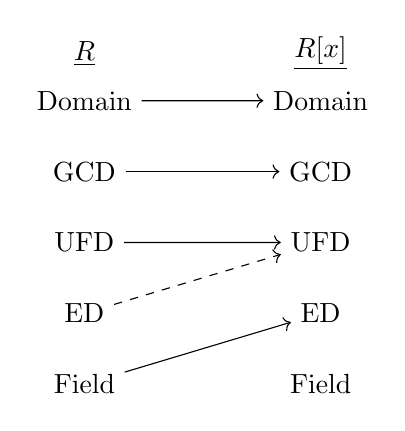
\begin{tikzpicture}[scale=0.3]
  \node (fld1) at (-5,0)  {Field};
  \node (fld2) at ( 5,0)  {Field};
  \node (ed1)  at (-5,3)  {ED};
  \node (ed2)  at ( 5,3)  {ED};
  \node (ufd1) at (-5,6)  {UFD};
  \node (ufd2) at ( 5,6)  {UFD};
  \node (gcd1) at (-5,9)  {GCD};
  \node (gcd2) at ( 5,9)  {GCD};
  \node (dom1) at (-5,12) {Domain};
  \node (dom2) at ( 5,12) {Domain};
  \node (lab1) at (-5,14) {\(\underline{R}\)};
  \node (lab2) at ( 5,14) {\(\underline{R[x]}\)};

  \draw [->] (fld1) edge (ed2);
  \draw [->, dashed] (ed1)  edge (ufd2);
  \draw [->] (ufd1) edge (ufd2);
  \draw [->] (gcd1) edge (gcd2);
  \draw [->] (dom1) edge (dom2);
\end{tikzpicture}
\end{center}

One might expect that detecting irreducibles and finding irreducible factorizations would be more difficult in \(\ZZ[x]\), say, than in \(\ZZ\), but in fact the opposite is true. This is ultimately due to the existence of the derivative on \(R[x]\) and to some other aspects of the structure of \(R[x]\) which will be explored later.

We've seen here that if \(R\) is a UFD, then \(R[x]\) is also a UFD, but have not seen any kind of algorithm which computes factorizations in \(R[x]\). In the exercises of this and the next section we construct algorithms which work in some important special cases, including \(\ZZ\) and \(\ZZ/(p)\).



  \chapter{Ideals and Quotients}
    \label{chap:quot}
    \newpage

    \section{Congruences}
      \label{sec:congruence}
      Recall the Construction Problem for rings: given a ring, we'd like to construct new rings out of its ``parts''.
So far we've seen several examples of how this can be done including by generating subrings, taking direct sums, constructing rings of fractions, and using polynomials.
This chapter is devoted to yet another method for building new rings out of old ones -- by constructing \emph{quotients}.
This idea is very frequently a stumbling block for beginning students of mathematics, so we will spend some time on it.
But our effort will be rewarded.
Quotient rings are an extremely powerful and natural idea, and more generally the concept of ``quotient'' used here is pervasive in other branches of math.
In a very specific sense quotient rings are the ``opposites'' of subrings.

Here is the basic idea: given a ring \(R\) and an equivalence relation \(\Phi\) on \(R\), we partition \(R\) into equivalence classes as \(R/\Phi\).
Now we attempt to define an arithmetic on \emph{equivalence classes} as follows.
\begin{enumerate}
\item Given two \(\Phi\)-\emph{classes}, say \(X\) and \(Y\) in \(R/\Phi\), first \textbf{choose} some representatives \(x \in X\) and \(y \in Y\).
Now compute the sum \(x+y\) in \(R\).
This element is in some other \(\Phi\)-class \(Z\) in \(R/\Phi\).
We define \(Z\) to be the sum of \(X\) and \(Y\).
\item Likewise, to multiply classes, we \textbf{choose} representatives, multiply in \(R\), and determine the class of the product.
\end{enumerate}
This is a fine idea, and in fact this is precisely how arithmetic works in \(\ZZ/(n)\).
But unfortunately there is a problem: the sum of two classes may depend on our \textbf{choice} of representatives.
Specifically, choosing one pair of representatives \(v_1\) and \(w_1\) may end up in one class, while another pair \(v_2\) \(w_2\) may end up in another class; see \autoref{fig:quot-bad} for an illustration.
\begin{figure}[h!]
\begin{center}
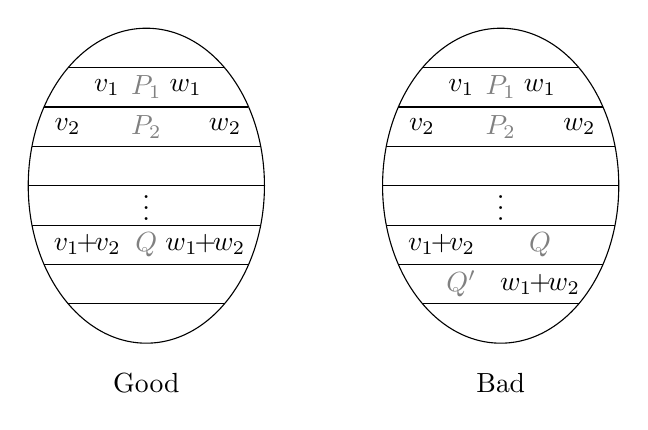
\begin{tikzpicture}[scale=0.5]
  \draw (3,4) ellipse (3 and 4);
  \draw (1.02,1) edge (4.98,1);
  \draw (0.40,2) edge (5.59,2);
  \draw (0.09,3) edge (5.90,3);
  \draw (0.00,4) edge (6.00,4);
  \draw (0.09,5) edge (5.90,5);
  \draw (0.40,6) edge (5.59,6);
  \draw (1.02,7) edge (4.98,7);
  \node at (3,3.65) {\(\vdots\)};
  \node at (2,6.5) {\(v_1\)};
  \node at (4,6.5) {\(w_1\)};
  \node at (1,5.5) {\(v_2\)};
  \node at (5,5.5) {\(w_2\)};
  \node at (1.5,2.5) {\(v_1\!\!+\!\!v_2\)};
  \node at (4.5,2.5) {\(w_1\!\!+\!\!w_2\)};
  \node at (3,6.5) [gray] {\(P_1\)};
  \node at (3,5.5) [gray] {\(P_2\)};
  \node at (3,2.5) [gray] {\(Q\)};
  \node at (3,-1) {Good};
  \draw (12,4) ellipse (3 and 4);
  \draw (10.02,1) edge (13.98,1);
  \draw (09.40,2) edge (14.59,2);
  \draw (09.09,3) edge (14.90,3);
  \draw (09.00,4) edge (15.00,4);
  \draw (09.09,5) edge (14.90,5);
  \draw (09.40,6) edge (14.59,6);
  \draw (10.02,7) edge (13.98,7);
  \node at (12,3.65) {\(\vdots\)};
  \node at (11,6.5) {\(v_1\)};
  \node at (13,6.5) {\(w_1\)};
  \node at (10,5.5) {\(v_2\)};
  \node at (14,5.5) {\(w_2\)};
  \node at (10.5,2.5) {\(v_1\!\!+\!\!v_2\)};
  \node at (13,1.5) {\(w_1\!\!+\!\!w_2\)};
  \node at (12,6.5) [gray] {\(P_1\)};
  \node at (12,5.5) [gray] {\(P_2\)};
  \node at (13,2.5) [gray] {\(Q\)};
  \node at (11,1.5) [gray] {\(Q^\prime\)};
  \node at (12,-1) {Bad};
\end{tikzpicture}
\caption{\label{fig:quot-bad} What can go wrong when making partitions into rings.}
\end{center}
\end{figure}
More concretely we can try this strategy by partitioning the set of integers into two sets; the primes \(P\) and the nonprimes \(N\).
We might try to compute the sum \(P+P\) using representatives \(2\) and \(3\); in this case \[ P + P = [2] + [3] = [2+3] = [5] = P. \]
But if we use representatives \(3\) and \(7\), we have \[ P + P = [3] + [7] = [3+7] = [10] = N. \]
This is a problem -- it means that this \(+\) operation is not well-defined.
To fix the problem, we just need to make sure our partition is chosen so that this bad thing never happens.

\begin{dfn}[Ring Congruence] \label{dfn:ring-congruence}
Let \(R\) be a ring.
An equivalence relation \(\Phi\) on \(R\) is called a \emph{congruence}\index{congruence} if the following hold.
\begin{proplist*}
\item If \(x_1 \mathrel{\Phi} x_2\) and \(y_1 \mathrel{\Phi} y_2\), then \((x_1+y_1) \mathrel{\Phi} (x_2+y_2)\).
\item If \(x_1 \mathrel{\Phi} x_2\) and \(y_1 \mathrel{\Phi} y_2\), then \((x_1 y_1) \mathrel{\Phi} (x_2 y_2)\).
\end{proplist*}
\end{dfn}

So a congruence is a particular kind of equivalence relation.
The congruence condition may at first glance seem to be very strong -- so strong that it is not immediately clear that interesting congruences should even exist.
(We will see that they do, and are abundant).

\begin{examples}
\item Let \(R\) be a ring.
Then the \emph{diagonal} relation \(\Delta = \{ (r,r) \mid r \in R \}\) and the \emph{universal} relation \(\nabla = \{ (r,s) \mid r,s \in R \}\) are both congruences.
These are called the \emph{trivial} congruences on \(R\).

\item The relation \(\Phi\) on \(\ZZ\) defined by \(r \mathrel{\Phi} s \Leftrightarrow n|(s-r)\) is a congruence.
In fact \(\ZZ\) here can be replaced by any commutative ring \(R\) and \(n\) by any fixed element of \(R\).
\end{examples}

\begin{prop}
Let \(R\) be a ring and \(\Phi\) an equivalence on \(R\).
\begin{proplist}
\item The operations \(+\) and \(\cdot\) on \(R/\Phi\) given by \[ [a] + [b] = [a+b] \quad \mathrm{and} \quad [a] \cdot [b] = [a \cdot b] \] are well-defined if and only if \(\Phi\) is a congruence.
\item In this case, \((R/\Phi, +, \cdot)\) is a ring, called the \emph{quotient} of \(R\) by \(\Phi\).
If \(R\) is commutative, then \(R/\Phi\) is commutative, and if \(R\) is unital, the \(R/\Phi\) is unital.
\end{proplist}
\end{prop}

\begin{proof}
\begin{inlineproplist}
\item If we want to be pedantic (and we do!), the precise operations on \(R/\Phi\) are \[ \mathsf{plus} = \left\{ \left(([a],[b]), [a+b]\right) \mid a,b \in R \right\} \] and \[ \mathsf{times} = \left\{ \left(([a],[b]), [ab]\right) \mid a,b \in R \right\}. \]
First, suppose \(\Phi\) is a congruence, and suppose we have elements \((([a_1],[b_1]),[a_1+b_1])\) and \((([a_2],[b_2]),[a_2+b_2])\) in \(\mathsf{plus}\) such that \([a_1] = [a_2]\) and \([b_1] = [b_2]\).
Then (by definition) \(a_1 \mathrel{\Phi} a_2\) and \(b_1 \mathrel{\Phi} b_2\).
Since \(\Phi\) is a congruence, \(a_1 + b_1 \mathrel{\Phi} a_2 + b_2\), and thus \([a_1 + b_1] = [a_2 + b_2]\); so \(\mathsf{plus}\) is well-defined.
A similar argument shows that \(\mathsf{times}\) is well-defined.
Conversely, suppose \(\mathsf{plus}\) and \(\mathsf{times}\) are well-defined.
If \(a_1 \mathrel{\Phi} a_2\) and \(b_1 \mathrel{\Phi} b_2\), then \([a_1] = [a_2]\) and \([b_1] = [b_2]\), so that \([a_1+b_1] = [a_1] + [b_1] = [a_2] + [b_2] = [a_2+b_2]\), and thus \(a_1+b_1 \mathrel{\Phi} a_2+b_2\).
Similarly we can show that \(a_1b_1 \mathrel{\Phi} a_2b_2\) so that \(\Phi\) is a congruence.
\item Showing that all 6 of the ring axioms is somewhat tedious; for instance, to show A1 note that if \(a,b,c \in R\), we have \[ ([a] + [b]) + [c] = [a+b] + [c] = [(a+b)+c] = [a+(b+c)] = [a] + [b+c] = [a] + ([b] + [c]). \]
Similarly if \(R\) is commutative then \( [a][b] = [ab] = [ba] = [b][a] \) for all \(a,b \in R\).
Finally, if \(R\) is unital, then evidently \([1_R]\) is a one in \(R/\Phi\).
\end{inlineproplist}
\end{proof}

Quotients are thus -- potentially -- a rich new source of examples of rings.
There are some potential problems, however.
First, it is not immediately clear how we can find interesting congruences.
Second, once we have a congruence, it is not clear how we can effectively detect when two elements of \(R\) are in the same \(\Phi\)-class.
This means that even detecting when two elements of \(R/\Phi\) are equal may be difficult -- which has important computational consequences.
Third, since quotient rings are sets of sets, the most natural way to define a mapping on \(R/\Phi\), in terms of class representatives, is fraught with danger.
We expect that finding well-defined homomorphisms from a quotient ring will be difficult.
Fortunately we will see that all three of these problems have nice resolutions.

As an example, what can we say about the ring \(\QQ[x]/(x^2 + 1)\)?
Using the division algorithm, every polynomial in \(\QQ[x]\) can be written as \((x^2+1)q(x) + r(x)\), where \(r\) is either 0, a nonzero constant, or a linear polynomial (@@@).



%---------%
\Exercises%
%---------%

\begin{exercise}
Let \(R\) be a ring, and let \(\Delta\) and \(\nabla\) denote the trivial and universal congruences on \(R\).
Show that \(R \cong R/\Delta\) and \(0 \cong R/\nabla\).
\end{exercise}


\begin{exercise}
(One-sided ideals)
\end{exercise}

      \newpage

    \section{Ideals}
      \label{sec:ideals}
      We've seen that special equivalence relations called \emph{congruences} can be used to build new rings out of old ones via the quotient construction.
Now we'd like to understand the congruences in more depth.
In this section we will see that the congruences on a ring correspond in a useful way to certain subrings.
First, we show that the congruence class of zero plays a very special role.

\begin{prop}
Let \(R\) be a ring and \(\Phi\) a congruence on \(R\), and let \(I\) be the \(\Phi\)-class of 0.
Then we have the following.
\begin{proplist}
\item \(I\) is a subring of \(R\).
\item \(I\) absorbs \(R\) under multiplication from either side.
That is, if \(a \in I\) and \(r \in R\), then \(ar \in I\) and \(ra \in I\).
\item Every \(\Phi\)-class is of the form \(r + I = \{ r+a \mid a \in I \}\) for some \(r \in R\).
In this case, \(r+I\) is called the \(r\)-\emph{coset}\index{coset} of \(I\).
\end{proplist}
\end{prop}

\begin{proof}
\begin{inlineproplist}
\item Using the Subring Criterion, certainly \(0_R \in [0_R]\), and if \(x,y \in [0_R]\), then \[ x-y \in [0_R] - [0_R] = [0_R] \quad \mathrm{and} \quad xy \in [0_R][0_R] = [0_R]. \]
\item If \(a \in [0_R]\) and \(r \in R\), then \[ ar \in [0_R][r] = [0_R] \quad \mathrm{and} \quad ra \in [r][0_R] = [0_R]. \]
\item Let \([r]\) be a \(\Phi\)-class; we claim that \([r] = r + I\).
To see this, note that if \(s \in [r]\), then \([s] = [r]\), so that \([s-r] = [0_R]\).
That is, \(s-r \in [0_R]\).
Say \(s-r = z\).
Then \(s = r+z \in r+I\).
Conversely, if \(s = r+z \in r+I\) then \(s-r \in [0_R]\), so that \([s] = [r]\) and thus \(s \in [r]\).
\end{inlineproplist}
\end{proof}

That is, if \(\Phi\) is a congruence then every class of \(\Phi\) is a coset of the class of zero.
This alone is an interesting observation, but it has a practical consequence as well.
Arithmetic in \(R/\Phi\) can be carried out in terms of coset representatives.

\begin{prop}
Let \(R\) be a ring, \(\Phi\) a congruence on \(R\), and \(I\) the \(\Phi\)-class of zero.
Then for all \(r,s \in R\), we have the following.
\begin{proplist}
\item \((r+I)+(s+I) = (r+s)+I\).
\item \((r+I) (s+I) = (r s)+I\).
\end{proplist}
\end{prop}

\begin{proof}
It's important to realize that the \(+\) symbol is used in three different senses here: the \(+\) in \(r+s\) is the plus in \(R\), the \(+\) between \(r+I\) and \(s+I\) is the plus in \(R/\Phi\), and the \(+\) in \(r+I\) is a structural symbol denoting cosets.
With this in mind, we have \[ (r+I)+(s+I) = [r] + [s] = [r+s] = (r+s)+I \] and \[ (r+I)(s+I) = [r][s] = [rs] = (rs)+I \] as claimed.
\end{proof}

Apparently the congruence class of zero is special, so we extract its properties in the following definition.

\begin{dfn}[Ideal]
Let \(R\) be a ring.
A subring \(I \subseteq R\) is called an \emph{ideal}\index{ideal} if \(I\) absorbs \(R\) under multiplication from both sides.
That is, if \(a \in I\) and \(r \in R\), then \(ar \in I\) and \(ra \in I\).
\end{dfn}

\begin{prop} \label{prop:ideal-conditions}
Let \(R\) be a ring and \(I \subseteq R\) a subset.
Then the following are equivalent.
\begin{proplist}
\item \label{prop:ideal-conditions:ideal} \(I\) is an ideal of \(R\).
\item \label{prop:ideal-conditions:congruence} The relation \(\Phi = \{ (r,s) \mid s-r \in I \}\) is a congruence on \(R\) with \([0_R] = I\).
We say \(\Phi\) is \emph{induced} by \(I\).
\item \label{prop:ideal-conditions:kernel} There is a surjective homomorphism \(\varphi : R \rightarrow S\) with \(\KER{\varphi} = I\).
(If \(R\) is unital, this \(\varphi\) can be chosen to be unital.)
\end{proplist}
\end{prop}

\begin{proof}
\begin{inlineproplist}
\item[\((\ref{prop:ideal-conditions:ideal} \Rightarrow \ref{prop:ideal-conditions:congruence})\)] (@@@)
\item[\((\ref{prop:ideal-conditions:congruence} \Rightarrow \ref{prop:ideal-conditions:kernel})\)]
\item[\((\ref{prop:ideal-conditions:kernel} \Rightarrow \ref{prop:ideal-conditions:ideal})\)] 
\end{inlineproplist} 
\end{proof}

\begin{examples}
\item The diagonal relation \(\Delta\) is a congruence on any ring \(R\), and the class of zero is \(\{0_R\}\).
So the cosets which comprise \(R/\Delta\) are of the form \[ r+[0_R] = r+\{0_R\} = \{ r+0_R \} = \{r\}; \] that is, \(\Delta\) is induced by the zero ideal and the elements of \(R/\Delta\) are singletons.
\item The universal relation \(\nabla\) is a congruence on any ring \(R\), and the class of zero is all of \(R\).
So there is only one coset in \(R/\nabla\): \([0_R] = R\).
\item Let \(R\) be a commutative ring and \(a \in R\) a fixed element.
If \(\Phi\) is the congruence given by \(r \mathrel{\Phi} s\) iff \(a|(s-r)\), then the class of zero is the set \[ [0_R] = \{ r \in R \mid a|r \} \] of all elements of \(R\) which are divisible by \(a\).
\end{examples}

Congruences and ideals are equivalent: every ideal induces a congruence, and every congruence is induced by an ideal.
For this reason from now on we will consider ideals alone and keep all congruences implicit.
Typically we abuse the notation by referring to a quotient ring \(R/I\) (with \(I\) an ideal) when we really mean \(R/\Phi\), where \(\Phi\) is the congruence induced by \(I\).

\begin{prop}[Ideal Criterion]
Let \(R\) be a ring.
A subset \(I \subseteq R\) is an ideal if and only if the following hold.
\begin{proplist*}
\item \(I\) is not empty.
\item \(I\) is closed under subtraction.
\item \(I\) absorbs \(R\) under multiplication from either side.
\end{proplist*}
\end{prop}

\begin{prop}[Unital Ideal Criterion]
Let \(R\) be a unital ring.
A subset \(I \subseteq R\) is an ideal if and only if \(I\) is not empty and \(a - rbs \in I\) whenever \(a,b \in I\) and \(r,s \in R\).
\end{prop}

\begin{proof}
(@@@)
\end{proof}



%---------%
\Exercises%
%---------%

\begin{exercise}
Let \(R\) be a ring such that \(R/(a)\) is finite for any nonzero \(a \in R\).
Define \(N : R \rightarrow \NN\) by \(N(a) = |R/(a)|\).
Show that \(N\) is a Euclidean norm on \(R\).
(@@@) is this true?
\end{exercise}

\begin{exercise}
Every ideal is a union of associate classes.
\end{exercise}

      \newpage

    \section{The Isomorphism Theorems}
      \label{sec:iso-thms}
      Defining a mapping on a quotient set is generally difficult, for the same reason that defining operations on a quotient set is difficult; the most natural thing to try is to define our mapping in terms of representatives, but this is generally not well-defined.

The first important result about quotient rings gives us a standard way to construct homomorphisms on a quotient ring that bypasses this difficulty. This result, known as the First Isomorphism Theorem, is due to Emmy Noether, and is an important tool in ring theory.

\begin{prop}[First Isomorphism Theorem for Rings]
Let \(R\) be a ring and \(I\) an ideal of \(R\), and suppose \(\varphi : R \rightarrow S\) is a ring homomorphism. If \(I \subseteq \KER{\varphi}\), then there is a ring homomorphism \(\overline{\varphi} : R/I \rightarrow S\) such that \(\overline{\varphi}(x + I) = \varphi(x)\). That is, \(\varphi = \overline{\varphi} \circ \pi_I\), so that the following diagram commutes.
\begin{center}
\begin{tikzcd}
R \arrow[r, "\varphi"] \arrow[d, "\pi_I"'] & S \\
R/I \arrow[ru, dashed, "\overline{\varphi}"'] &
\end{tikzcd}
\end{center}
\end{prop}

\begin{proof}
(@@@)
\end{proof}

\begin{cor}
If \(\varphi : R \rightarrow S\) is a homomorphism then the induced map \(\overline{\varphi} : R/\KER{\varphi} \rightarrow S\) is injective. If \(\varphi\) is surjective then \(\overline{\varphi}\) is an isomorphism.
\end{cor}

Another way to state FIT is as follows: If \(\varphi\) is a ring homomorphism and \(I\) an ideal contained in the kernel of \(\varphi\), then \(\varphi\) factors through the projection induced by \(I\). This terminology is inspired by the commutative diagram associated to FIT, in which we literally have \(\varphi = \overline{\varphi} \circ \pi\).

Two other nice results relate the ideals of a ring to ideals of its subrings and of its quotients. In a nutshell, every ideal in \(R/I\) corresponds nicely to an ideal in \(R\). Ideals in a subring \(S \subseteq R\) correspond (kind of) to ideals in \(R\), but the correspondence is not nearly as nice. So while subrings and quotient rings are opposite concepts in a concrete sense, there is a fundamental asymmetry. This is not too surprising; for instance every domain (which tend to have lots of nontrivial ideals) can be embedded in a field (which we will see have none).

\begin{prop}[Second Isomorphism Theorem for Rings]
Let \(R\) be a ring, with \(S \subseteq R\) a subring and \(I \subseteq R\) an ideal. Then we have the following.
\begin{proplist}
\item \(S \cap I\) is an ideal in \(S\),
\item \(I\) is an ideal in \(S + I\), and
\item \(S/(S \cap I)\) is isomorphic to \((S+I)/I\).
\end{proplist}
\end{prop}

\begin{proof}
(@@@)
\end{proof}

\begin{prop}[Third Isomorphism Theorem]
Let \(R\) be a ring with \(I \subseteq R\) an ideal.
\begin{proplist}
\item If \(J \subseteq R\) is an ideal such that \(I \subseteq J\), then \(I\) is an ideal in \(J\).
\item If \(K \subseteq R/I\) is an ideal, then there is an ideal \(J \subseteq R\) such that \(I \subseteq J\) and \(K = J/I\).
\item If \(J \subseteq R\) is an ideal and \(I \subseteq J \subseteq R\), then \((R/I)/(J/I)\) is isomorphic to \(R/J\).
\end{proplist}
\end{prop}

\begin{proof}
(@@@)
\end{proof}

      \newpage

    \section{Ideal Arithmetic}
      \label{sec:ideal-lattice}
      The ideals of a ring enjoy an arithmetic of their own.

\begin{dfn}
If \(R\) is a ring, \(\IDEALS{R}\) denotes the set of all ideals of \(R\).
\end{dfn}

\begin{prop}
Let \(R\) be a ring and \(I, J \subseteq R\) ideals. Then the subsets
\begin{eqnarray*}
I + J & = & \{ a+b \mid a \in I, b \in J \} \\
I   J & = & \left\{ \sum_{i=0}^n a_i b_i \mid n \in \NN, a_i \in I, b_i \in J \right\}
\end{eqnarray*}
are both ideals of \(R\), called the \emph{ideal sum}\index{sum!of ideals} and \emph{ideal product}\index{product!of ideals} respectively.
\end{prop}

\begin{prop}
Let \(R\) be a ring and \(I,J,K \subseteq R\) ideals. Then we have the following.
\begin{proplist}
\item \(IJ \subseteq I \cap J\) and \(I,J \subseteq I+J\).
\item \(I+(J+K) = (I+J)+K\)
\item \(I+0 = 0+I = I\)
\item \(I+R = R+I = R\)
\item \(I(JK) = (IJ)K\)
\item \(I0 = 0I = 0\)
\item \(IR = RI = I\)
\item \(I(J+K) = IJ+IK\) and \((I+J)K = IK+JK\)
\end{proplist}
\end{prop}



%---------%
\Exercises%
%---------%


      \newpage

    \section{Maximal Ideals}
      \label{sec:max-ideals}
      \begin{dfn}
Let \(R\) be a ring.
An ideal \(I \subseteq R\) is called \emph{maximal}\index{maximal!ideal} if there does not exist an ideal \(J \subseteq R\) such that \(I \subsetneq J \subsetneq R\).
\end{dfn}

\begin{prop}
A ring \(R\) is a field if and only if the zero ideal is maximal.
\end{prop}

\begin{proof}
First let \(R\) be a field, and suppose \(I \subsetneq R\) is a nonzero ideal; say \(x \in I\) is not zero.
Now \(x\) is a unit in \(R\), so that \(I = R\).
Conversely, suppose the zero ideal is maximal in \(R\).
(@@@)
\end{proof}

\begin{prop}
An ideal \(I\) in a ring \(R\) is maximal if and only if \(R/I\) is a field.
\end{prop}

\begin{prop}[Krull]
Every unital ring has at least one maximal ideal.
\end{prop}

\begin{proof}
(@@@)
\end{proof}

      \newpage

    \section{Generating Sets}
      \label{sec:gen-sets}
      \begin{prop}
Let \(R\) be a ring, and let \(\mathcal{I}\) be a collection of ideals of \(R\).
Then \(\bigcap \mathcal{I}\) is an ideal of \(R\).
\end{prop}

Not every subset of \(R\) is an ideal; in fact most aren't.
However, \emph{every subset of \(R\) is contained in a unique smallest ideal}.

\begin{prop}[Generated Ideals]
Let \(R\) be a ring and \(A \subseteq R\) a subset.
We define the set \((A)\) by \[ (A) = \bigcap \{ I \mid I \subseteq R\ \mathrm{is\ an\ ideal\ and}\ A \subseteq I \}. \]
Then the following hold.
\begin{proplist}
\item \((A)\) is an ideal of \(R\).
\item If \(A\) is an ideal of \(R\), then \((A) = A\).
\item \(A \subseteq (A)\).
\item If \(I\) is an ideal of \(R\) and \(A \subseteq R\), then \((A) \subseteq I\).
\end{proplist}
We call \((A)\) the ideal of \(R\) \emph{generated by} \(A\).
If \(I\) is an ideal and \(I = (A)\), we say that \(A\) is a \emph{generating set}\index{generating set!of an ideal} for \(I\).
\end{prop}

\begin{prop}
Let \(R\) be a ring and \(A\) and \(B\) be subsets of \(R\).
Then the following hold.
\begin{proplist}
\item \((A) + (B) = (A \cup B)\)
\item \((A)(B) = (ab \mid a \in A, b \in B)\)
\end{proplist}
\end{prop}

\begin{dfn}
Let \(I\) be an ideal of a ring.
\begin{enumerate}
\item We say \(I\) is \emph{finitely generated} if there is a finite set \(A\) such that \(I = (A)\).
\item We say a subset \(A\) is a \emph{minimal generating set} of \(I\) if \(I = (A)\) and whenever \(B \subsetneq A\) is a proper subset, \((B) \subsetneq (A)\) is also a proper subset.
\end{enumerate}
\end{dfn}

Important note: ``minimal'' here does not mean \emph{smallest size}, but rather \emph{contains no redundant elements}.
In general an ideal will have many minimal generating sets, and these may have very different cardinalities.
For example, the ideal \((3) \subseteq \ZZ\) is minimally generated by the set \(\{3\}\), but also by the set \(\{6,15\}\).

\begin{prop}
Let \(R\) be a commutative unital ring and \(A\) a subset of \(R\).
Then \[ (A) = \{ \sum_{i=0}^n r_ia_i \mid n \in \NN, r_i \in R, a_i \in A \}. \]
That is, in a commutative unital ring, the ideal generated by \(A\) consists of all finite \(R\)-linear combinations of elements of \(A\).
\end{prop}

\begin{proof}
(@@@ type this)
\end{proof}



%---------%
\Exercises%
%---------%

\begin{exercise}
Show that for any natural number \(k \geq 1\), the ideal \((3\) in \(\ZZ\) has a minimal generating set containing \(k\) elements.
\end{exercise}

      \newpage

    \section{Prime Ideals}
      \newpage

    \section{The Chinese Remainder Theorem}
      \newpage

    \phantomsection
    \section*{Summary of \autoref{chap:quot}}
      \addcontentsline{toc}{section}{Summary}%&%
      \input{src/ring/4.X-summary.tex}

  \chapter{Fields}

    \section{Subfields and Extensions}


\setcounter{dummycounter}{\value{section}}%&%
\appendix
\setcounter{section}{\value{dummycounter}}%&%

  \chapter{Rings with Absolute Value}
    \label{chap:abs-val}
    In these notes we've been carefully avoiding the use of the real numbers, \(\RR\).
Even though \(\RR\) is in some ways the most familiar example of a ring -- most of your mathematical training so far has taken place inside \(\RR\) -- our intuitive familiarity with \(\RR\) is deceptive.
The real numbers are \textbf{very strange}, and it is far too easy to coast through calculus without appreciating how strange they are.

Nevertheless, the real numbers (and the closely related complex numbers) are extremely useful, and we lose something important by ignoring them completely.
In this appendix we will fill this gap by constructing the real numbers from scratch.
It turns out that if we approach this construction with the right amount of abstraction, we can build not just the real numbers \(\RR\) but a whole family of interesting rings.

    \newpage

    \section{Just Enough Metric Topology}
      \label{sec:ring-with-abs-val}
      Recall that if \(R\) is a ring and \(A\) any nonempty set, then the set \(R^A\) of all mappings \(A \rightarrow R\) is a ring with pointwise arithmetic.
As a special case, an element \(\alpha\) of the ring \(R^\NN\) is called a \emph{sequence}\index{sequence} of \(R\).
We will denote the image of a sequence \(\alpha\) at a particular natural number index \(i\) by \(\alpha_i\) rather than the usual \(\alpha(i)\).
Given \(r \in R\), we denote by \(\TILDE{r}\) the constant sequence with value \(r\); that is, \(\TILDE{r}_i = r\) for all \(i\).

It's about to start looking a lot like calculus in here.
Do not be alarmed; we will only do as much analysis as is absolutely necessary.
This section proceeds at a much faster pace.

\begin{dfn}[Absolute Value] \label{dfn:abs-val}
Let \(R\) be a ring.
A mapping \(v : R \rightarrow \QQ\) is called a (rational) \emph{absolute value}\index{absolute value} if the following properties are satisfied.
\begin{proplist}
\item \(v(x) \geq 0\) for all \(x \in R\).
\item \(v(x) = 0\) if and only if \(x = 0_R\).
\item \(v(xy) = v(x)v(y)\) for all \(x,y \in R\).
\item The Triangle Inequality: \(v(x+y) \leq v(x) + v(y)\) for all \(x,y \in R\).
\end{proplist}
\end{dfn}

The basic example of an absolute value on a ring is the usual absolute value on \(\QQ\).
For now, in the interest of brevity, we will save any more examples for the exercises or the later sections of this chapter.

\begin{prop} \label{prop:abs-val-basics}
If \(R\) is a ring with absolute value \(v\) then we have the following.
\begin{proplist}
\item If \(x,y \in R\) and \(xy = 0_R\), then either \(x = 0_R\) or \(y = 0_R\).
\item \label{prop:abs-val-basics:reverse-ti} \(v(x-y) \geq v(x) - v(y)\) for all \(x,y \in R\).
\item \(v(-x) = v(x)\) for all \(x \in R\).
\item If \(R\) is unital, then \(v(1_R) = 1\).
\item If \(R\) is unital and \(u \in R\) a unit, then \(v(u^{-1}) = 1/v(u)\).
\end{proplist}
\end{prop}

\begin{proof}
\begin{inlineproplist}
\item If \(xy = 0_R\), then \(v(x)v(y) = v(xy) = 0\).
Since \(\QQ\) is a field, either \(v(x) = 0\) (so that \(x = 0_R\)) or \(v(y) = 0\) (so that \(y = 0_R\)).
\item We have \[ v(x) = v(x-y+y) \leq v(x-y) + v(y) \] so that \(v(x) - v(y) \leq v(x-y)\).
\item Note that \(v(-x)^2 = v((-x)^2) = v(x^2) = v(x)^2\), so that \(v(-x)^2 - v(x)^2 = 0\) in \(\QQ\).
Thus \((v(-x) + v(x))(v(-x) - v(x)) = 0\).
Since \(\QQ\) is a field, one of these factors must be zero.
But note that \(v(-x) + v(x) = 0\) can only be true if \(v(x) = v(-x) = 0\) since the value of \(v\) is nonnegative.
In this case we have \(x = 0_R = -x\), and so \(v(x) = v(-x)\).
If \(x \neq 0_R\), then \(v(x) + v(-x)\) is nonzero, so that \(v(x) - v(-x) = 0\), and thus \(v(-x) = v(x)\).
\item Note that \(v(1_R) = v(1_R^2) = v(1_R)^2\), so that \(v(1_R)(1 - v(1_R)) = 0\).
Since \(1_R \neq 0_R\), we have \(v(1_R) \neq 0\), and thus \(1 - v(1_R) = 0\).
So \(v(1_R) = 1\).
\item We have \(1 = v(1_R) = v(uu^{-1}) = v(u)v(u^{-1})\) as needed.
\end{inlineproplist}
\end{proof}

\begin{dfn}[Bounded Sequence]
Let \(R\) be a ring with absolute value \(v\).
A sequence \(\alpha : \NN \rightarrow R\) is called \emph{bounded}\index{sequence!bounded} if there is a positive rational number \(B\) such that \(v(\alpha_i) \leq B\) for all \(i \in \NN\).
In this case we say that \(B\) is a \emph{bound} of \(\alpha\).
\end{dfn}

For instance the constant sequence \(r_i = r\) is bounded since \(v(\TILDE{r}_i) \leq v(r) < v(r) + 1\).

\begin{prop}
Let \(R\) be a ring and \(v\) an absolute value on \(R\).
Then the set \(\mathcal{B}\) of all bounded sequences of \(R\) is a subring of the ring of all sequences of \(R\).
If \(R\) is unital, then \(\mathcal{B}\) is a unital subring.
\end{prop}

\begin{proof}
Following the Subring Criterion (\ref{prop:subring-criterion}), it suffices to show that \(\mathcal{B}\) is nonempty and closed under multiplication and subtraction.
\begin{inlineproplist}
\item Every constant sequence, such as \(\TILDE{0_R}\), is bounded.
So \(\mathcal{B}\) is nonempty.
\item Suppose \(\alpha\) and \(\beta\) are bounded sequences, with \(v(\alpha_i) \leq B_\alpha\) and \(v(\beta_i) \leq B_\beta\) for all natural numbers \(i\).
Then for all \(i\) we have  \[ v((\alpha\beta)_i) = v(\alpha_i \beta_i) = v(\alpha_i)v(\beta_i) \leq B_\alpha B_\beta, \] using the fact that \(v(x)\) is nonnegative for all \(x\).
So \(B_\alpha B_\beta\) is a bound of \(\alpha\beta\).
\item Suppose again that \(\alpha\) and \(\beta\) are bounded by \(B_\alpha\) and \(B_\beta\), respectively, and let \(i \in \NN\).
Then we have \[ v((\alpha - \beta)_i) = v(\alpha_i - \beta_i) \leq v(\alpha_i) + v(-\beta_i) = v(\alpha_i) + v(\beta_i) \leq B_\alpha + B_\beta. \] So \(B_\alpha + B_\beta\) is a bound of \(\alpha - \beta\).
\end{inlineproplist}
Finally, if \(R\) is unital, then \(\mathcal{B}\) contains the constant sequence \(\TILDE{1_R}\), which is the one in \(R^\NN\).
\end{proof}

\begin{dfn}[Convergent Sequence]
Let \(R\) be a ring with absolute value \(v\).
A sequence \(\alpha : \NN \rightarrow R\) is called \emph{convergent}\index{sequence!convergent} if there is an \(\ell \in R\) such that for every rational number \(\varepsilon > 0\), there exists a natural number \(N\) such that \(v(\alpha_i - \ell) < \varepsilon\) whenever \(i \geq N\).
In this case we say \(\ell\) is a \emph{limit}\index{limit!of a sequence} of the sequence \(\alpha\).
\end{dfn}

\begin{prop}
The limit of a convergent sequence is unique.
If \(\alpha\) is a convergent sequence then we denote its (unique) limit by \(\LIM{\alpha}\) or by \(\LIM[n]{\alpha_n}\).
\end{prop}

\begin{proof}
Suppose \(\alpha\) is a convergent sequence with limits \(\ell_1\) and \(\ell_2\), and suppose further that \(\ell_1 \neq \ell_2\).
In particular we have \(v(\ell_1 - \ell_2) > 0\).
Choose a rational number \(\varepsilon\) such that \(0 < \varepsilon < v(\ell_1 - \ell_2)/2\).
Since \(\alpha\) is convergent with limits \(\ell_1\) and \(\ell_2\), there exists a natural number \(k\) sufficiently large that \(v(\alpha_k - \ell_1) < \varepsilon\) and \(v(\alpha_k - \ell_2) < \varepsilon\).
Then we have \[ v(\ell_1 - \ell_2) = v(\ell_1 - \alpha_k + \alpha_k - \ell_2) \leq v(\ell_1 - \alpha_k) + v(\alpha_k - \ell_2) < 2\varepsilon < v(\ell_1 - \ell_2), \] a contradiction.
\end{proof}

\begin{prop} \label{prop:convergent-seq-subset}
Let \(R\) be a ring with absolute value \(v\).
Then among the sequences of \(R\) we have the following.
\begin{proplist}
\item \label{prop:convergent-seq-subset:constant} Every constant sequence is convergent.
\item \label{prop:convergent-seq-subset:bounded} Every convergent sequence is bounded.
\end{proplist}
\end{prop}

\begin{proof}
\begin{inlineproplist}
\item Let \(r \in R\).
Given a rational number \(\epsilon > 0\), set \(N = 0\).
Now for all natural numbers \(i \geq N\) we have \[ v(\TILDE{r}_i - r) = v(r - r) = v(0_R) = 0 < \varepsilon, \] so \(\TILDE{r}\) is convergent with limit \(r\).
\item Suppose \(\alpha\) is a convergent sequence with limit \(\ell\).
Since \(1 > 0\), there is a natural number \(N\) with the property that \(v(\alpha_i - \ell) < 1\) for all \(i \geq N\).
Using \sref{prop:abs-val-basics}{reverse-ti}, we have \(v(\alpha_i) - v(\ell) < 1\), and thus \(v(\alpha_i) < v(\ell) + 1\) for all \(i \geq N\).
Now set \[ B = \max(v(\alpha_0), v(\alpha_1), \ldots, v(\alpha_{N-1}), v(\ell) + 1). \]
By construction we have \(v(\alpha_i) \leq B\) for all \(i \in \NN\); thus \(B\) is a bound of \(\alpha\).
\end{inlineproplist}
\end{proof}

\begin{prop} \label{prop:convergent-sequences-are-subring}
Let \(R\) be a ring with absolute value \(v\).
Then the set \(\mathcal{V}\) of all convergent sequences of \(R\) is a subring of the ring of all sequences of \(R\).
If \(R\) is unital, then \(\mathcal{V}\) is a unital subring.
\end{prop}

\begin{proof}
Again following the Subring Criterion (\ref{prop:subring-criterion}) it suffices to show that \(\mathcal{V}\) is nonempty and closed under subtraction and multiplication.
\begin{inlineproplist}
\item Every constant sequence, such as \(\TILDE{0_R}\), is convergent, so that \(\mathcal{V}\) is not empty.
\item Suppose \(\alpha\) and \(\beta\) are convergent sequences with \(\LIM{\alpha} = \ell_\alpha\) and \(\LIM{\beta} = \ell_\beta\), and let \(\varepsilon > 0\) be an arbitrary rational number.
Note that \(\varepsilon/2\) is positive, so that (since \(\alpha\) and \(\beta\) are convergent) there exist natural numbers \(N_\alpha\) and \(N_\beta\) such that \[ v(\alpha_i - \ell_\alpha) < \varepsilon/2 \quad \mathrm{when}\ i \geq N_\alpha \] and \[ v(\beta_i - \ell_\beta) < \varepsilon/2 \quad \mathrm{when}\ i \geq N_\beta. \]
Set \(N = \max(N_\alpha, N_\beta)\).
Now if \(i \geq N\), we have the following.
\begin{eqnarray*}
v\left((\alpha - \beta)_i - (\ell_\alpha - \ell_\beta)\right)
 & = & v(\alpha_i - \beta_i - \ell_\alpha + \ell_\beta) \\
 & = & v\left((\alpha_i - \ell_\alpha) + (\ell_\beta - \beta_i)\right) \\
 & \leq & v(\alpha_i - \ell_\alpha) + v(\ell_\beta - \beta_i) \\
 & < & \frac{\varepsilon}{2} + \frac{\varepsilon}{2} \\
 & = & \varepsilon.
\end{eqnarray*}
Thus \(\alpha - \beta\) is convergent.
\item Again suppose \(\alpha\) and \(\beta\) are convergent sequences with \(\LIM{\alpha} = \ell_\alpha\) and \(\LIM{\beta} = \ell_\beta\), and let \(\varepsilon > 0\).
By \sref{prop:convergent-seq-subset}{bounded}, \(\alpha\) is also bounded; say \(v(\alpha_i) \leq B_\alpha\) for all \(i\).
Now let \(U = \max\left(B_\alpha, v(\ell_\beta)\right)\).
Since \(U > 0\), we have \(\varepsilon/(2U) > 0\).
Since \(\alpha\) and \(\beta\) are convergent, there exist natural numbers \(N_\alpha\) and \(N_\beta\) such that \[ v(\alpha_i - \ell_\alpha) < \frac{\varepsilon}{2U} \quad \mathrm{when}\ i \geq N_\alpha \] and \[ v(\beta_i - \ell_\beta) < \frac{\varepsilon}{2U} \quad \mathrm{when}\ i \geq N_\beta. \]
Let \(N = \max(N_\alpha, N_\beta)\).
Then if \(i \geq N\) we have the following.
\begin{eqnarray*}
v((\alpha\beta)_i - \ell_\alpha \ell_\beta)
 & = & v(\alpha_i\beta_i - \ell_\alpha \ell_\beta) \\
 & = & v(\alpha_i\beta_i - \alpha_i \ell_\beta + \alpha_i \ell_\beta - \ell_\alpha \ell_\beta) \\
 & = & v\left( \alpha_i(\beta_i - \ell_\beta) + (\alpha_i - \ell_\alpha)\ell_\beta \right) \\
 & \leq & v(\alpha_i)v(\beta_i - \ell_\beta) + v(\alpha_i - \ell_\alpha)v(\ell_\beta) \\
 & < & U \cdot \frac{\varepsilon}{2U} + \frac{\varepsilon}{2U} \cdot U \\
 & = & \varepsilon.
\end{eqnarray*}
(Note that \(R\) is not necessarily commutative!)
So \(\alpha\beta\) is convergent.
\end{inlineproplist}
Finally, if \(R\) is unital, then \(\mathcal{V}\) contains the constant sequence \(\TILDE{1_R}\), which is the one in \(R^\NN\).
\end{proof}

\begin{cor}
If \(\alpha\) and \(\beta\) are convergent sequences, then so are \(\alpha - \beta\), \(\alpha \beta\), and \(\alpha + \beta\), and in fact we have \(\LIM{\alpha - \beta} = \LIM{\alpha} - \LIM{\beta}\), \(\LIM{\alpha\beta} = \LIM{\alpha}\LIM{\beta}\), and \(\LIM{\alpha + \beta} = \LIM{\alpha} + \LIM{\beta}\).
In particular, letting \(\mathcal{V}\) denote the set of convergent sequences of \(R\), the mapping \(\lim : \mathcal{V} \rightarrow R\) is a ring homomorphism.
\end{cor}

\begin{dfn}[Cauchy Sequence]
Let \(R\) be a ring with absolute value \(v\).
A sequence \(\alpha : \NN \rightarrow R\) is called \emph{cauchy}\index{sequence!cauchy} if for every rational number \(\varepsilon > 0\) there exists a natural number \(M\) such that \(v(\alpha_j - \alpha_i) < \varepsilon\) whenever \(i,j \geq M\).
\end{dfn}

\begin{prop} \label{prop:cauchy-seq-subset}
Let \(R\) be a ring with absolute value \(v\).
Then among the sequences of \(R\) we have the following.
\begin{proplist}
\item \label{prop:cauchy-seq-subset:convergent} Every convergent sequence is cauchy.
\item \label{prop:cauchy-seq-subset:bounded} Every cauchy sequence is bounded.
\end{proplist}
\end{prop}

\begin{proof}
\begin{inlineproplist}
\item Let \(\alpha\) be a convergent sequence with limit \(\ell\).
Let \(\varepsilon > 0\).
Now \(\varepsilon/2 > 0\), and since \(\alpha\) is convergent there exists a natural number \(N\) such that \(v(\alpha_i - \ell) < \varepsilon/2\) whenever \(i,j \geq N\).
Setting \(M = N\), whenever \(i \geq M\), we have \[ v(\alpha_j - \alpha_i) = v(\alpha_j - \ell + \ell - \alpha_i) \leq v(\alpha_j - \ell) + v(\ell - \alpha_i) < \frac{\varepsilon}{2} + \frac{\varepsilon}{2} = \varepsilon. \]
Thus \(\alpha\) is cauchy.
\item Suppose \(\alpha\) is cauchy.
Since \(1 > 0\), there is a natural number \(M\) such that \(v(\alpha_j - \alpha_i) < 1\) whenever \(i,j \geq M\).
In particular, we have \(v(\alpha_j - \alpha_M) < 1\) whenever \(j \geq M\).
Using \sref{prop:abs-val-basics}{reverse-ti} we have \(v(\alpha_j) - v(\alpha_M) < 1\), so that \(v(\alpha_j) < v(\alpha_M) + 1\) whenever \(j \geq M\).
Now set \[ B = \max(v(\alpha_0), v(\alpha_1), \ldots, v(\alpha_{M-1}, v(\alpha_M) + 1). \]
We then have \(v(\alpha_i) < B\) for all \(i \in \NN\), so that \(B\) is a bound for \(\alpha\).
\end{inlineproplist}
\end{proof}

\begin{prop}
Let \(R\) be a ring with absolute value \(v\).
Then the set \(\mathcal{C}\) of all cauchy sequences of \(R\) is a subring of the ring of all sequences of \(R\).
If \(R\) is unital, then \(\mathcal{C}\) is a unital subring.
\end{prop}

\begin{proof}
Again we follow the Subring Criterion (\ref{prop:subring-criterion}), showing that \(\mathcal{C}\) is not empty and closed under subtraction and multiplication.
\begin{inlineproplist}
\item Every constant sequence, such as \(\TILDE{0_R}\), is convergent, hence cauchy.
So \(\mathcal{C}\) is not empty.
\item Suppose \(\alpha\) and \(\beta\) are cauchy, and let \(\varepsilon > 0\).
Now \(\varepsilon/2 > 0\), and so there exist natural numbers \(M_\alpha\) and \(M_\beta\) such that \[ v(\alpha_j - \alpha_i) < \varepsilon/2 \quad \mathrm{when}\ i,j \geq M_\alpha \] and \[ v(\beta_j - \beta_i) < \varepsilon/2 \quad \mathrm{when}\ i,j \geq M_\beta. \]
Let \(M = \max(M_\alpha, M_\beta)\).
Now if \(i,j \geq M\), we have the following.
\begin{eqnarray*}
v\left( (\alpha - \beta)_j - (\alpha - \beta)_i \right)
 & = & v(\alpha_j - \beta_j - \alpha_i + \beta_j) \\
 & = & v\left( (\alpha_j - \alpha_i) + (\beta_i - \beta_j) \right) \\
 & \leq & v(\alpha_j - \alpha_i) + v(\beta_j - \beta_i) \\
 & < & \frac{\varepsilon}{2} + \frac{\varepsilon}{2} \\
 & = & \varepsilon.
\end{eqnarray*}
Thus \(\alpha - \beta\) is cauchy as needed.
\item Suppose \(\alpha\) and \(\beta\) are cauchy, and choose a rational number \(\varepsilon > 0\).
Now by \sref{prop:cauchy-seq-subset}{bounded}, both \(\alpha\) and \(\beta\) are bounded; say \(B_\alpha\) and \(B_\beta\) are rational numbers such that \(v(\alpha_i) \leq B_\alpha\) and \(v(\beta_i) \leq B_\beta\) for all \(i\).
Now \(\varepsilon/(2B_\beta) > 0\), and since \(\alpha\) is cauchy, there is a natural number \(M_\alpha\) such that \(v(\alpha_j - \alpha_i) < \varepsilon/(2B_\alpha)\) whenever \(i,j \geq M_\alpha\).
Similarly, there is a natural number \(M_\beta\) such that \(v(\beta_j - \beta_i) < \varepsilon/(2B_\alpha)\) whenever \(i,j \geq M_\beta\).
Now let \(M = \max(M_\alpha,M_\beta)\).
Then if \(i,j \geq M\), we have the following.
\begin{eqnarray*}
v\left((\alpha\beta)_j - (\alpha\beta)_i\right)
 & = & v(\alpha_j\beta_j - \alpha_i\beta_i) \\
 & = & v(\alpha_j\beta_j - \alpha_j\beta_i + \alpha_j\beta_i - \alpha_i\beta_i) \\
 & = & v\left( \alpha_j(\beta_j - \beta_i) + (\alpha_j - \alpha_i)\beta_i \right) \\
 & \leq & v(\alpha_j)v(\beta_j - \beta_i) + v(\alpha_j - \alpha_i)v(\beta_i) \\
 & < & B_\alpha \frac{\varepsilon}{2B_\alpha} + \frac{\varepsilon}{2B_\beta} B_\beta \\
 & = & \varepsilon.
\end{eqnarray*}
Thus \(\alpha\beta\) is cauchy as needed.
\end{inlineproplist}
Finally, if \(R\) is unital then the constant sequence \(\TILDE{1_R}\) is cauchy.
\end{proof}

\begin{prop} \label{prop:cauchy-bound-away-from-zero}
If \(\alpha\) is a cauchy sequence which \emph{does not} converge to \(0_R\), then there is a rational number \(\delta > 0\) and a natural number \(T\) such that \(v(\alpha_i) \geq \delta\) for all \(i \geq T\).
That is, if a cauchy sequence does not converge to zero, the it is eventually bounded away from zero.
\end{prop}

\begin{proof}
Since \(\alpha\) does not converge to zero, there exists a rational number \(\varepsilon\) such that for every natural number \(N\), there exists an index \(i \geq N\) such that \(v(\alpha_i) \geq \varepsilon\).
(This is the negation of the statement ``\(\alpha\) converges to zero''.)
Now since \(\alpha\) is cauchy, and since \(\varepsilon/2 > 0\), there is a natural number \(M\) such that \(v(\alpha_j - \alpha_i) < \varepsilon/2\) whenever \(i,j \geq M\).
There exists an index \(k \geq M\) such that \(v(\alpha_k) \geq \varepsilon\).
Now \(v(\alpha_k - \alpha_i) < \varepsilon/2\) for all \(i \geq M\), and so for all \(i\) we have the following.
\begin{eqnarray*}
\varepsilon & \leq & v(\alpha_k) \\
 & = & v(\alpha_k - \alpha_i + \alpha_i) \\
 & \leq & v(\alpha_k - \alpha_i) + v(\alpha_i) \\
 & < & \varepsilon/2 + v(\alpha_i).
\end{eqnarray*}
So \(v(\alpha_i) > \varepsilon/2\).
The result then holds with \(\delta = \varepsilon/2\) and \(T = M\).
\end{proof}

So we have a chain of inclusions among the sequences: \[ \mathrm{convergent} \subseteq \mathrm{cauchy} \subseteq \mathrm{bounded} \subseteq \mathrm{sequences}. \]
Moreover this is not just a chain of sub\emph{sets}, but of sub\emph{rings}, meaning that we get some additional ring-theoretic results for free.
We say that a sequence is \emph{null}\index{sequence!null} if it converges to \(0_R\).
Then we can show that the set of null sequences is an \emph{ideal} in the ring of bounded sequences.

\begin{prop}
Let \(R\) be a ring with absolute value \(v\).
Then the set \(\mathcal{N}\) of all null sequences of \(R\) is a two-sided ideal in the ring \(\mathcal{B}\) of all bounded sequences of \(R\).
In particular, \(\mathcal{N}\) is also a two-sided ideal in the ring \(\mathcal{C}\) of all cauchy sequences and the ring \(\mathcal{V}\) of all convergent sequences.
\end{prop}

\begin{proof}
Certainly we have \(\mathcal{N} \subseteq \mathcal{V} \subseteq \mathcal{C} \subseteq \mathcal{B}\).
Now we establish that \(\mathcal{N}\) is a subring of \(R^\NN\).
Using the Subring Criterion, we certainly have \(\TILDE{0_R} \in \mathcal{N}\), and if \(\alpha,\beta \in \mathcal{N}\) then \(\alpha - \beta\) and \(\alpha\beta\) are convergent by \ref{prop:convergent-sequences-are-subring} and we have \[ \LIM{\alpha - \beta} = \LIM{\alpha} - \LIM{\beta} = 0_R - 0_R = 0_R \] and \[ \LIM{\alpha\beta} = \LIM{\alpha}\LIM{\beta} = 0_R \cdot 0_R = 0_R \] as needed.
It remains to be seen that \(\mathcal{N}\) absorbs \(\mathcal{B}\) under multiplication from either side.
To this end, suppose \(\alpha\) is a bounded sequence of \(R\) with \(v(\alpha_i) \leq B\) for all \(i\), and that \(\zeta\) is a null sequence.
Let \(\varepsilon > 0\).
Now \(\varepsilon/B > 0\), and since \(\zeta\) converges to \(0_R\), there exists a natural number \(N\) such that \(v(\alpha_i) < \varepsilon/B\) whenever \(i \geq N\).
Now for all \(i \geq N\) we have \[ v((\alpha\zeta)_i) = v(\alpha_i \zeta_i) = v(\alpha_i)v(\zeta_i) \leq \frac{\varepsilon}{B} B = \varepsilon \] and similarly \(v((\zeta\alpha)_i) < \varepsilon\).
So \(\alpha\zeta\) and \(\zeta\alpha\) are null sequences as needed.
\end{proof}

\begin{prop}
The set of null sequences is a prime ideal in the set of cauchy sequences.
That is, if \(\alpha\) and \(\beta\) are cauchy sequences and \(\alpha\beta\) converges to \(0_R\), then either \(\alpha\) or \(\beta\) must converge to \(0_R\).
\end{prop}

\begin{proof}
Suppose \(\alpha\) and \(\beta\) are cauchy and that \(\alpha\beta\) converges to \(0_R\).
Suppose further without loss of generality that \(\alpha\) does not converge to \(0_R\).
By \ref{prop:cauchy-bound-away-from-zero}, there exists a rational number \(\delta > 0\) and a natural number \(T\) such that \(v(\alpha_i) \geq \delta\) whenever \(i \geq T\).
Now let \(\varepsilon > 0\); then also \(\varepsilon\delta > 0\).
Since \(\alpha\beta\) converges to \(0_R\), there is a natural number \(N\) such that \(v(\alpha_i\beta_i) < \varepsilon\delta\) whenever \(i \geq N\).
If we set \(N_1 = \max(N, T)\), then whenever \(i \geq N_1\) in fact we have \[ \delta v(\beta_i) \leq v(\alpha_i)v(\beta_i) = v(\alpha_i\beta_i) < \delta\varepsilon; \] since \(\delta > 0\), we have \(v(\beta_i) < \varepsilon\) for all \(i \geq N_1\).
Thus \(\beta\) converges to \(0_R\).
\end{proof}

We are finally prepared for the punchline of this section.

\begin{dfn}[Cauchy Completion]
Let \(R\) be a ring with absolute value \(v\).
Letting \(\mathcal{C}\) denote the set of cauchy sequences on \(R\) and \(\mathcal{N}\) the set of null sequences on \(R\), we define \(\VALCOMP{R}{v} = \mathcal{C}/\mathcal{N}\) to be the \emph{cauchy completion}\index{cauchy completion} of \(R\) with respect to \(v\).
\end{dfn}

\begin{prop}
\begin{proplist}
\item If \(R\) is a commutative unital ring then \(\VALCOMP{R}{v}\) is an integral domain.
\item Let \(R\) be a ring with absolute value \(v\).
Then the mapping \(\iota : R \rightarrow \VALCOMP{R}{v}\) given by \(\iota(r) = \TILDE{r} + N\) is an injective ring homomorphism.
\end{proplist}
\end{prop}

\begin{proof}
(@@@)
\end{proof}



%---------%
\Exercises%
%---------%

\begin{exercise}
Let \(k\) be a field and let \(R\) be the field of rational functions in one variable over \(k\).
Show that \(v(p/q) = 2^{deg p - deg q}\) is an absolute value on \(R\).
(@@@) is this true?
\end{exercise}

      \newpage

    \section{The Real Numbers}
      \label{sec:reals}
      We are now prepared to define the set of real numbers; (most of) the heavy lifting is already done.

\begin{dfn}[Real Numbers] \label{dfn:real-numbers}
The usual absolute value \(|\cdot|\) on the set \(\QQ\) of rational numbers is an absolute value in the sense of \ref{dfn:abs-val}, and so the constructions of \autoref{sec:ring-with-abs-val} are immediately available.
We define the set of \emph{real numbers}\index{real numbers} \(\RR\) to be the cauchy completion \(\VALCOMP{\QQ}{|\cdot|}\) of \(\QQ\) with respect to \(|\cdot|\).
Since \(\QQ\) is a field, \(\RR\) is also a field.
\end{dfn}

Doing arithmetic in \(\RR\) is a bit awkward because elements of \(\RR\) are equivalence classes of cauchy sequences.
Even detecting whether two specific real numbers are equal to each other is difficult.

\begin{dfn}
Given two cauchy sequences of rational numbers, \(\alpha\) and \(\beta\), we say that \(\alpha \leq \beta\) if either \(\beta - \alpha\) converges to 0 or there exists a natural number \(W\) such that \(\alpha_i < \beta_i\) for all \(i \geq W\).
\end{dfn}

\begin{prop}
If \(\alpha\), \(\overline{\alpha}\), \(\beta\), and \(\overline{\beta}\) are cauchy sequences of rational numbers such that \(\alpha - \overline{\alpha}\) and \(\beta - \overline{\beta}\) converge to zero and \(\alpha \leq \beta\), then \(\overline{\alpha} \leq \overline{\beta}\).
\end{prop}

\begin{proof}
If \(\beta - \alpha\) converges to zero, then we have \[ 0 = \LIM{\beta - \alpha} - \LIM{\beta - \overline{\beta}} + \LIM{\alpha - \overline{\alpha}} = \LIM{\beta - \alpha - \beta + \overline{\beta} + \alpha - \overline{\alpha}} = \LIM{\overline{\beta} - \overline{\alpha}}, \] so that \(\overline{\alpha} \leq \overline{\beta}\).
Suppose instead that \(\beta - \alpha\) does not converge to zero.
Since \(\alpha \leq \beta\), there is a natural number \(W\) such that \(\alpha_i < \beta_i\) whenever \(i \geq W\).
Also, by \ref{prop:cauchy-bound-away-from-zero}, there is a rational number \(\delta\) and a natural number \(T\) such that \(|\beta_i - \alpha_i| \geq \delta\) whenever \(i \geq T\).
Since \(\delta/2 > 0\) and \(\alpha - \overline{\alpha}\) converges to 0, there is a natural number \(N_\alpha\) such that \(|\alpha_i - \overline{\alpha}_i| < \delta/2\) when \(i \geq N_\alpha\).
Similarly there is an \(N_\beta\) such that \(|\beta_i - \overline{\beta}_i| < \delta/2\) when \(i \geq N_\beta\).

Let \(W_1 = \max(W, T, N_\alpha, N_\beta)\).
Then for all \(i \geq W_1\), we have \(\alpha_i < \beta_i\), and thus \(\beta_i - \alpha_i = |\beta_i - \alpha_i| \geq \delta\).
Now we have the following.
\begin{eqnarray*}
\delta - (\overline{\beta}_i - \overline{\alpha}_i)
 & \leq & (\beta_i - \alpha_i) - (\overline{\beta}_i - \overline{\alpha}_i) \\
 & = & (\beta_i - \overline{\beta}_i) + (\overline{\alpha}_i - \alpha_i) \\
 & \leq & |\beta_i - \overline{\beta}_i| + |\overline{\alpha}_i - \alpha_i| \\
 & < & \delta/2 + \delta/2 \\
 & = & \delta.
\end{eqnarray*}
So we have \(0 < \overline{\beta}_i - \overline{\alpha}_i\), and thus \(\overline{\alpha}_i < \overline{\beta}_i\) for all \(i \geq W_1\).
Thus \(\overline{\alpha} \leq \overline{\beta}\).
\end{proof}

\begin{cor}
We have a relation \(\leq\) on \(\RR\) defined as follows: given \([\alpha]\) and \([\beta]\) in \(\RR\), we say that \([\alpha] \leq [\beta]\) if either \(\beta - \alpha\) converges to 0 or there is a natural number \(W\) such that \(\alpha_i < \beta_i\) whenever \(i \geq W\).
We say \([\alpha] < [\beta]\) if \([\alpha] \leq [\beta]\) and \([\alpha] \neq [\beta]\).
\end{cor}

\begin{prop}
The relation \(\leq\) on \(\RR\) has the following properties.
\begin{proplist}
\item \([\alpha] \leq [\alpha]\) for all \([\alpha] \in \RR\).
\item If \([\alpha] \leq [\beta]\) and \([\beta] \leq [\alpha]\), then \([\alpha] = [\beta]\).
\item If \([\alpha] \leq [\beta]\) and \([\beta] \leq [\gamma]\), then \([\alpha] \leq [\gamma]\).
\item If \([\alpha]\) is a real number, then either \([\alpha] > [\TILDE{0}]\), \([\alpha] = [\TILDE{0}]\), or \([\alpha] < [\TILDE{0}]\).
\end{proplist}
\end{prop}

\begin{proof}
\begin{inlineproplist}
\item Since \(\alpha - \alpha\) converges to 0, we have \([\alpha] \leq [\alpha]\).
\item Suppose \([\alpha] \leq [\beta]\) and \([\beta] \leq [\alpha]\).
Now if either \(\beta - \alpha\) or \(\alpha - \beta\) converge to zero, we have \([\alpha] = [\beta]\).
So we assume that this does not happen.
In this case we have natural numbers \(W_1\) and \(W_2\) such that \(\alpha_i < \beta_i\) whenever \(i \geq W_1\) and \(\beta_i < \alpha_i\) whenever \(i \geq W_2\).
But if \(i \geq \max(W_1, W_2)\), then \(\alpha_i < \beta_i < \alpha_i\), a contradiction.
So we have \([\alpha] = [\beta]\) as needed.
\item If either \(\beta - \alpha\) or \(\gamma - \beta\) converge to zero, we have \([\alpha] = [\beta]\) or \([\beta] = [\gamma]\); in either case, \([\alpha] \leq [\gamma]\).
Now suppose that neither \(\beta - \alpha\) nor \(\gamma - \beta\) converges to zero.
Then there exist natural numbers \(W_1\) and \(W_2\) such that \(\alpha_i < \beta_i\) when \(i \geq W_1\) and \(\beta_i < \gamma_i\) when \(i \geq W_2\).
Letting \(W = \max(W_1,W_2)\), whenever \(i \geq W\) we have \[ \gamma_i - \alpha_i = \gamma_i - \beta_i + \beta_i - \alpha_i > 0 \] so that \(\alpha_i < \gamma_i\).
Thus \([\alpha] \leq [\gamma]\) as needed.
\item Let \([\alpha]\) be a real number and suppose \([\alpha] \neq [\TILDE{0}]\).
That is, \(\alpha\) does not converge to zero.
By \ref{prop:cauchy-bound-away-from-zero}, there is a rational number \(\delta\) and a natural number \(T\) such that \(|\alpha_i| \geq \delta\) when \(i \geq T\).
Also, since \(\alpha\) is cauchy, there exists a natural number \(M\) such that \(|\alpha_j - \alpha_i| < \delta\) when \(i,j \geq M\).
Set \(W = \max(T,M)\).
We will show that if \(i,j \geq W\), then \(\alpha_i\) and \(\alpha_j\) must have the same sign in \(\QQ\) (either both positive or both negative).
To this end, suppose \(\alpha_j > 0\) and \(\alpha_i < 0\).
On one hand we have \(|\alpha_j - \alpha_i| < \delta\).
But on the other hand we have \(\alpha_j \geq \delta\) and \(-\alpha_i \geq \delta\).
So \[ 2\delta \leq \alpha_j - \alpha_i \leq |\alpha_j - \alpha_i| < \delta, \] a contradiction.
Likewise if \(\alpha_j < 0\) and \(\alpha_i > 0\) then \[ 2\delta \leq \alpha_i - \alpha_j \leq |\alpha_i - \alpha_j| < \delta. \] That is, for all \(i \geq W\), the \(\alpha_i\) have the same sign, either positive or negative.
In the first case we have \([\TILDE{0}] \leq [\alpha]\), and in the second case \([\alpha] \leq [\TILDE{0}]\).
But since \([\alpha] \neq [\TILDE{0}]\), in fact either \([\alpha] < [\TILDE{0}]\) or \([\alpha] > [\TILDE{0}]\).
\end{inlineproplist}
\end{proof}

\begin{prop}
\begin{proplist}
\item If \([\alpha] \leq [\beta]\) then \([\alpha] + [\gamma] \leq [\beta] + [\gamma]\).
\item If \([\TILDE{0}] \leq [\alpha]\) and \([\TILDE{0}] \leq [\beta]\) then \([\TILDE{0}] \leq [\alpha][\beta]\).
\item \([\TILDE{0}] < [\TILDE{1}]\).
\end{proplist}
\end{prop}

\begin{proof}
\begin{inlineproplist}
\item If \(\beta - \alpha\) converges to 0, then \([\alpha] = [\beta]\) and the result holds.
If \(\beta - \alpha\) does not converge to 0, then there is an index \(W\) such that \(\alpha_i < \beta_i\) for all \(i \geq W\).
For all such \(i\), we have \(\alpha_i + \gamma_i < \beta_i + \gamma_i\), so that \([\alpha] + [\gamma] \leq [\beta] + [\gamma]\) as claimed.
\item If either \([\alpha]\) or \([\beta]\) converge to zero, then \([\alpha][\beta] = [\TILDE{0}]\).
Suppose instead that neither converges to zero.
Then there exist natural numbers \(W_\alpha\) and \(W_\beta\) such that \(\alpha_i > 0\) when \(i \geq W_\alpha\) and \(\beta_i > 0\) when \(i \geq W_\beta\).
Let \(W = \max(W_\alpha, W_\beta)\).
Then for all \(i \geq W\), we have \(\alpha_i \beta_i > 0\), so that \([\TILDE{0}] \leq [\alpha][\beta]\) as claimed.
\item Certainly \(0 < 1\), so that \([\TILDE{0}] \leq [\TILDE{1}]\).
Since \(1 \neq 0\), \([\TILDE{0}] \neq [\TILDE{1}]\).
\end{inlineproplist}
\end{proof}

\begin{prop}
(@@@) every nonempty set with an upper bound has a least upper bound.
\end{prop}

\begin{prop} \label{prop:rr-axioms}
There is a field \(\RR\), whose elements are called \emph{real numbers}, which comes with a linear order relation \(\leq\) having the following properties.
\begin{proplist}
\item \(0 < 1\).
\item If \(\alpha, \beta, \gamma \in \RR\) such that \(\alpha \leq \beta\), then \(\alpha + \gamma \leq \beta + \gamma\).
\item If \(\alpha, \beta \in \RR\) such that \(0 \leq \alpha\) and \(0 \leq \beta\), then \(0 \leq \alpha\beta\).
\item If \(S \subseteq \RR\) is a nonempty set which has an upper bound, then \(S\) has a \emph{least} upper bound.
\end{proplist}
\end{prop}

Working directly with equivalence classes of cauchy sequences - that is, real numbers - can get awkward very fast.
Fortunately, there is a better way! It turns out that \ref{prop:rr-axioms} \emph{characterizes} the real numbers, in the sense that any other field \(F\) with a linear order relation \(\preceq\) that \emph{also} satisfies the properties in \ref{prop:rr-axioms} must be isomorphic to \(\RR\).
This means that any theorem which can be proved about \(\RR\) can be proved using the properties of \ref{prop:rr-axioms}, together with the definition of field and linear order, as a list of ``axioms'', rather than the complicated construction using cauchy sequences.
In fact this is the approach typically taken by high school textbooks, if you pay close attention.
With this in mind, why should we bother explicitly constructing \(\RR\) in the first place? The (potential) problem is that we can make lists of axioms all day and derive theories based on them, but without a concrete \emph{model} of those axioms we cannot assume that the axioms are consistent with each other.
This is a great example of the abstract and concrete points of view each bringing something useful to the table: the axioms are nice to work with, and the model tells us the axioms describe something interesting.

\begin{prop}[Bolzano's Theorem for Polynomials]
Let \(p(x) \in \RR[x]\).
If \(a\) and \(b\) are real numbers such that \(a < b\) and \(p(a)\) and \(p(b)\) have opposite signs, then there exists a real number \(c\) such that \(p(c) = 0\).
\end{prop}

\begin{proof}
Suppose, without loss of generality, that \(f(a) < 0\) and \(f(b) > 0\).
Now define the set \(S = \{ x \in [a,b] \mid f(x) \leq 0 \}\).
Certainly \(S\) is not empty, since \(f(a) < 0\).
Moreover, \(S\) has an upper bound, since \(x < b\) for all \(x \in S\).
Thus \(S\) has a least upper bound, say \(c \in S\).
(@@@)
\end{proof}

\begin{cor} \mbox{}
\begin{proplist}
\item If \(p(x) \in \RR[x]\) has odd degree, then \(p(x)\) has a root in \(\RR\).
\item If \(\alpha \in \RR\) is positive, then \(q(x) = x^2 - \alpha\) has a unique positive root in \(\RR\), denoted \(\sqrt{\alpha}\).
\end{proplist}
\end{cor}

\begin{proof}
(@@@)
\end{proof}

      \newpage

    \section{The \emph{p}-adic Numbers}

  \chapter{Posets}
    \newpage

    \section{Posets and Zorn's Lemma}
      \label{sec:zorn}
      \begin{dfn}[Poset]
A \emph{partially ordered set} or \emph{poset}\index{poset} is a set \(P\) equipped with a binary relation \(\preceq\) having the following properties.
\begin{proplist}
\item[PO1.] \(x \preceq x\) for all \(x \in P\).
\item[PO2.] If \(x \preceq y\) and \(y \preceq x\), then \(x = y\).
\item[PO3.] If \(x \preceq y\) and \(y \preceq z\), then \(x \preceq z\).
\end{proplist}
\end{dfn}

\begin{dfn}
Let \(P\) be a poset.
\begin{proplist}
\item A \emph{chain}\index{chain} is a mapping \(x : \NN \rightarrow P\) which is order-preserving; that is, such that \(x_i \leq x_j\) whenever \(i \leq j\).
\item Let \(S \subseteq P\) be a subset.
An element \(b \in P\) is called an \emph{upper bound}\index{upper bound} of \(S\) if \(s \preceq b\) for all \(s \in S\).
\item An element \(m \in P\) is called \emph{maximal} if whenever \(x \in P\) such that \(m \preceq x\), in fact \(x = m\).
In other words, the inequality \(m \preceq x\) has only the trivial solution.
\end{proplist}
\end{dfn}

We take the following statement as an axiom, which for historical reasons is called a lemma.

\begin{axiom}[Zorn's Lemma]
If \(P\) is a nonempty poset in which every chain has an upper bound, then \(P\) has at least one maximal element.
\end{axiom}

Note that Zorn's Lemma tells us nothing about how such maximal elements are to be \emph{found}, only that they exist.
In this sense it is a nonconstructive statement very similar to the Well-Ordering Property of natural numbers; proofs which use Zorn may be slick, but cannot generally be turned into algorithms.

In practice we occasionally need to show that some ``extreme'' doodad having certain properties must exist, and there are two basic ways to do this.
The first and usually preferable way is to explicitly construct an example of such a doodad.
But this is not always possible, or may not be possible at the desired level of generality; in this case we use the second way: Zorn's Lemma.
This requires us to capture our ``extreme'' doodads as the maximal elements of an appropriate poset.
For example, in many cases it is easy to show that a \emph{particular} ring such as \(\ZZ\) or \(\QQ[x]\) has maximal ideals.
But to show that \emph{every} ring has maximal ideals, by far the easiest strategy is to use Zorn's Lemma in the poset of ideals.

Here is a concrete example.
Suppose we want to prove that every nonempty set \(A\) has maximal proper subsets; that is, subsets \(B \subsetneq A\) such that the inequality \(B \subseteq X \subsetneq A\) has no nontrivial solutions.
It is straightforward enough to construct an example -- we can show that \(B = A \setminus \{x\}\), where \(x \in A\), is a maximal proper subset.
For the sake of illustration let's suppose that constructing this example is very difficult, so we must instead use Zorn's Lemma.
That proof proceeds as follows.
\begin{proplist}
\item Verify that the set \(P = \{ B \in \POW{A} \mid B \neq A \}\) of proper subsets of \(A\) is partially ordered by set containment.
This follows from the basic properties of \(\subseteq\).
\item Verify that \(P\) is not empty.
Since \(A \neq \varnothing\) and \(\varnothing \subseteq A\), we have \(\varnothing \in P\).
\item Verify that every chain in \(P\) has an upper bound.
Suppose \(X_i\) is a chain of proper subsets of \(A\); we need to show that \(\{ X_i \mid i \in \NN \}\) has an upper bound.
Usually this step involves some kind of union; in this case we use \(B = \bigcup X_i\).
Clearly \(X_i \subseteq B\) for all \(i \in \NN\).
But to show that \(B\) is an upper bound of \(X_i\) we have to make sure that \(B\) is actually in \(P\).
(This is an important but easy-to-forget step!)
Certainly \(B \subseteq A\); suppose this containment is not proper, so that \(B = A\).
So every element of \(A\) is in one of the \(X_i\).
(@@@) This example is broken!
\end{proplist}

It is possible that a poset has maximal elements, but there exist chains with no upper bound -- that is, the converse of Zorn's Lemma is not true.



%---------%
\Exercises%
%---------%

\begin{exercise}
(@@@) The set \(\NN\) of natural numbers is a poset under the usual \(\leq\) relation.
However, this poset has chains with no upper bound, such as \(x_n = 2n\).
Thus Zorn's Lemma does not apply.
\end{exercise}

      \newpage

    \section{The Axiom of Choice}


\backmatter
  \printindex

\end{document}
